\documentclass[]{article}
\usepackage{lmodern}
\usepackage{amssymb,amsmath}
\usepackage{ifxetex,ifluatex}
\usepackage{fixltx2e} % provides \textsubscript
\ifnum 0\ifxetex 1\fi\ifluatex 1\fi=0 % if pdftex
  \usepackage[T1]{fontenc}
  \usepackage[utf8]{inputenc}
\else % if luatex or xelatex
  \ifxetex
    \usepackage{mathspec}
  \else
    \usepackage{fontspec}
  \fi
  \defaultfontfeatures{Ligatures=TeX,Scale=MatchLowercase}
\fi
% use upquote if available, for straight quotes in verbatim environments
\IfFileExists{upquote.sty}{\usepackage{upquote}}{}
% use microtype if available
\IfFileExists{microtype.sty}{%
\usepackage{microtype}
\UseMicrotypeSet[protrusion]{basicmath} % disable protrusion for tt fonts
}{}
\usepackage[margin=1in]{geometry}
\usepackage{hyperref}
\hypersetup{unicode=true,
            pdftitle={PROYECTO PIRHI},
            pdfborder={0 0 0},
            breaklinks=true}
\urlstyle{same}  % don't use monospace font for urls
\usepackage{graphicx,grffile}
\makeatletter
\def\maxwidth{\ifdim\Gin@nat@width>\linewidth\linewidth\else\Gin@nat@width\fi}
\def\maxheight{\ifdim\Gin@nat@height>\textheight\textheight\else\Gin@nat@height\fi}
\makeatother
% Scale images if necessary, so that they will not overflow the page
% margins by default, and it is still possible to overwrite the defaults
% using explicit options in \includegraphics[width, height, ...]{}
\setkeys{Gin}{width=\maxwidth,height=\maxheight,keepaspectratio}
\IfFileExists{parskip.sty}{%
\usepackage{parskip}
}{% else
\setlength{\parindent}{0pt}
\setlength{\parskip}{6pt plus 2pt minus 1pt}
}
\setlength{\emergencystretch}{3em}  % prevent overfull lines
\providecommand{\tightlist}{%
  \setlength{\itemsep}{0pt}\setlength{\parskip}{0pt}}
\setcounter{secnumdepth}{5}

%%% Use protect on footnotes to avoid problems with footnotes in titles
\let\rmarkdownfootnote\footnote%
\def\footnote{\protect\rmarkdownfootnote}

%%% Change title format to be more compact
\usepackage{titling}

% Create subtitle command for use in maketitle
\newcommand{\subtitle}[1]{
  \posttitle{
    \begin{center}\large#1\end{center}
    }
}

\setlength{\droptitle}{-2em}
  \title{Protocolo técnico-social de priorización de la inversión en mejoramiento de la eficiencia de conducción hídrica.}
  \pretitle{\vspace{\droptitle}\centering\huge}
  \posttitle{\par}
  \author{}
  \preauthor{}\postauthor{}
  \date{}
  \predate{}\postdate{}

\usepackage{geometry}
\geometry{letterpaper}
\usepackage{graphicx}
\usepackage{amssymb}
\usepackage{hyperref}
\usepackage{titlesec}
\usepackage{appendix}  
\usepackage{booktabs}
\usepackage{longtable}
\usepackage{multirow}
\usepackage{subcaption}
\usepackage{rotating}

\usepackage{fontspec,xltxtra,xunicode}
\defaultfontfeatures{Mapping=tex-text}
\setmainfont[		
 BoldFont={Century Gothic Bold}, 
 ItalicFont={Century Gothic Italic},
 BoldItalicFont={Century Gothic Bold Italic}
 ]{Century Gothic}
 
 \usepackage[labelfont=bf,font=small,justification=justified]{caption}[2008/04/01] %numeracion con punto y no dos puntos
\DeclareCaptionLabelSeparator{punto}{. } %numeracion con punto
\captionsetup{labelsep=punto} %numeracion con punto
 

\renewcommand{\figurename}{Figura}
\renewcommand{\tablename}{Cuadro} 
\renewcommand{\contentsname}{Tabla de contenidos\\} 
\renewcommand{\listfigurename}{Índice de figuras\\}
\renewcommand{\listtablename}{Índice de cuadros\\} 
\renewcommand{\appendixname}{Anexos}
\renewcommand{\appendixtocname}{Anexos}
\renewcommand{\appendixpagename}{Anexos}
\renewcommand{\thefootnote}{\fnsymbol{footnote}} % numeración por símbolos

\titleformat*{\section}{\normalsize\bfseries}
\titleformat*{\subsection}{\normalsize\bfseries}
\titleformat*{\subsubsection}{\normalsize\bfseries}

\usepackage{fancyvrb}
\newcommand{\VerbBar}{|}
\newcommand{\VERB}{\Verb[commandchars=\\\{\}]}
\DefineVerbatimEnvironment{Highlighting}{Verbatim}{commandchars=\\\{\}}
% Add ',fontsize=\small' for more characters per line
\usepackage{color}
\usepackage{framed}
\usepackage{tabulary}
\definecolor{shadecolor}{RGB}{248,248,248}
\newenvironment{Shaded}{\begin{snugshade}}{\end{snugshade}}
\newcommand{\KeywordTok}[1]{\textcolor[rgb]{0.13,0.29,0.53}{\textbf{#1}}}
\newcommand{\DataTypeTok}[1]{\textcolor[rgb]{0.13,0.29,0.53}{#1}}
\newcommand{\DecValTok}[1]{\textcolor[rgb]{0.00,0.00,0.81}{#1}}
\newcommand{\BaseNTok}[1]{\textcolor[rgb]{0.00,0.00,0.81}{#1}}
\newcommand{\FloatTok}[1]{\textcolor[rgb]{0.00,0.00,0.81}{#1}}
\newcommand{\ConstantTok}[1]{\textcolor[rgb]{0.00,0.00,0.00}{#1}}
\newcommand{\CharTok}[1]{\textcolor[rgb]{0.31,0.60,0.02}{#1}}
\newcommand{\SpecialCharTok}[1]{\textcolor[rgb]{0.00,0.00,0.00}{#1}}
\newcommand{\StringTok}[1]{\textcolor[rgb]{0.31,0.60,0.02}{#1}}
\newcommand{\VerbatimStringTok}[1]{\textcolor[rgb]{0.31,0.60,0.02}{#1}}
\newcommand{\SpecialStringTok}[1]{\textcolor[rgb]{0.31,0.60,0.02}{#1}}
\newcommand{\ImportTok}[1]{#1}
\newcommand{\CommentTok}[1]{\textcolor[rgb]{0.56,0.35,0.01}{\textit{#1}}}
\newcommand{\DocumentationTok}[1]{\textcolor[rgb]{0.56,0.35,0.01}{\textbf{\textit{#1}}}}
\newcommand{\AnnotationTok}[1]{\textcolor[rgb]{0.56,0.35,0.01}{\textbf{\textit{#1}}}}
\newcommand{\CommentVarTok}[1]{\textcolor[rgb]{0.56,0.35,0.01}{\textbf{\textit{#1}}}}
\newcommand{\OtherTok}[1]{\textcolor[rgb]{0.56,0.35,0.01}{#1}}
\newcommand{\FunctionTok}[1]{\textcolor[rgb]{0.00,0.00,0.00}{#1}}
\newcommand{\VariableTok}[1]{\textcolor[rgb]{0.00,0.00,0.00}{#1}}
\newcommand{\ControlFlowTok}[1]{\textcolor[rgb]{0.13,0.29,0.53}{\textbf{#1}}}
\newcommand{\OperatorTok}[1]{\textcolor[rgb]{0.81,0.36,0.00}{\textbf{#1}}}
\newcommand{\BuiltInTok}[1]{#1}
\newcommand{\ExtensionTok}[1]{#1}
\newcommand{\PreprocessorTok}[1]{\textcolor[rgb]{0.56,0.35,0.01}{\textit{#1}}}
\newcommand{\AttributeTok}[1]{\textcolor[rgb]{0.77,0.63,0.00}{#1}}
\newcommand{\RegionMarkerTok}[1]{#1}
\newcommand{\InformationTok}[1]{\textcolor[rgb]{0.56,0.35,0.01}{\textbf{\textit{#1}}}}
\newcommand{\WarningTok}[1]{\textcolor[rgb]{0.56,0.35,0.01}{\textbf{\textit{#1}}}}
\newcommand{\AlertTok}[1]{\textcolor[rgb]{0.94,0.16,0.16}{#1}}
\newcommand{\ErrorTok}[1]{\textcolor[rgb]{0.64,0.00,0.00}{\textbf{#1}}}
\newcommand{\NormalTok}[1]{#1}
\usepackage{graphicx,grffile}
\makeatletter
\def\maxwidth{\ifdim\Gin@nat@width>\linewidth\linewidth\else\Gin@nat@width\fi}
\def\maxheight{\ifdim\Gin@nat@height>\textheight\textheight\else\Gin@nat@height\fi}
\makeatother
\usepackage{booktabs}
\usepackage{longtable}
\usepackage{array}
\usepackage{multirow}
\usepackage[table]{xcolor}
\usepackage{wrapfig}
\usepackage{float}
\usepackage{colortbl}
\usepackage{pdflscape}
\usepackage{tabu}
\usepackage{threeparttable}
\usepackage[normalem]{ulem}
\usepackage[none]{hyphenat}
\usepackage{multicol}
\usepackage{tabularx}
\usepackage{rotating}
\usepackage{colortbl}
\usepackage{lscape}
\usepackage{footnote}
\usepackage{pdfpages}

% Regla con color
\makeatletter
\let\old@rule\@rule
\def\@rule[#1]#2#3{\textcolor{rulecolor}{\old@rule[#1]{#2}{#3}}}
\makeatother
% Cambiar color de regla
\definecolor{rulecolor}{RGB}{183,183,183}

% Color para las letras del título
\definecolor{casinegro}{RGB}{71,71,71}

\begin{document}
\sloppy 

\newgeometry{left=3cm,bottom=0cm,top=1cm,right=3cm}

\begin{titlepage}

\begin{figure} [H]
  
\includegraphics[width=.2\textwidth]{Logo/bg_gob_logo.png}
\end{figure}

\fontsize{15}{0} \selectfont{\textbf{\textcolor{casinegro}{``PLANIFICACIÓN DE LA INVERSIÓN EN REVESTIMIENTOS HÍDRICOS"}}} \vspace*{.1in}\\ % el inicio de comillas simples es ` y de doble es de ``.
\fontsize{15}{0} \selectfont{\textcolor{casinegro}{FIC-R 2016}}\\
\rule{10cm}{.05cm}
\vspace*{.1in}
\hspace*{.2in}

\fontsize{14}{0} \selectfont{\textcolor{casinegro}{Universidad de La Serena}} \vspace*{.1in}\\
\fontsize{14}{0} \selectfont{\textbf{\textcolor{casinegro}{Región de Coquimbo}}}

\vspace*{.1in}

\begin{figure}[H]
  \centering
\begin{subfigure}[c]{.2\textwidth}
  
\includegraphics[width=\textwidth]{Logo/GOB_RGB.png}
\end{subfigure}
\hfill
\begin{subfigure}[c]{.23\textwidth}
  
\includegraphics[width=\textwidth]{Logo/uls.png} 
\end{subfigure}
\end{figure}
\vspace*{4in}

\begin{figure}[H]
  \centering
\begin{subfigure}{.74\textwidth}
   \fontsize{14}{0} \selectfont{\textcolor{casinegro}{Mayo 2018}} \\
   {\definecolor{rulecolor}{named}{casinegro}\rule[-3mm]{10cm}{.05cm}}
\end{subfigure}
\hfill
\begin{subfigure}{.25\textwidth}
\hfill
  
\includegraphics[width=\textwidth]{Logo/lgore.pdf} 
\end{subfigure}
\end{figure}


\end{titlepage}

\restoregeometry


\begin{table}[!htb]
\centering \vspace*{2.5in}
\arrayrulecolor{cyan}
\begin{tabular}{|l|l|l|l|}
    \hline
    \multicolumn{3}{|c|}{\multirow{2}{8cm}{\centering \textbf{INFORME DE AVANCE TÉCNICO} \\
    \textbf{FIC REGIONAL} }} & \textbf{Fecha de emisión:}\\
    \cline{4-4}
    \multicolumn{3}{|c|}{\multirow{2}{8cm}} &  Diciembre 2018\\
    \hline
    \textbf{Fecha de inicio:}  &\textbf{Fecha de término:} &\textbf{N° de informe:} &\textbf{Duración:}\\
     20/Diciembre/2017 & 20/Octubre/2019 & 2 & 22 meses\\
    \hline
    \textbf{Nombre del proyecto:} & \multicolumn{3}{|l|}{\textbf{Planificación de la Inversión en Recursos Hídricos}}\\
    \hline
    \multirow{4}{4cm}{\textbf{Financiamiento:}} & \textbf{Monto total del proyecto:} & \multicolumn{2}{c|}{\centering M\$ 222.188}\\
    \cline{2-4}
    & \multirow{2}{4cm}{\textbf{Aporte FIC-R:}} & \multicolumn{2}{c|}{\textbf{Año 1:} M\$ 90.040}\\
    \cline{3-4}
    & & \multicolumn{2}{c|}{\textbf{Año 2:} M\$ 109.928}\\
    \cline{2-4}
    & \textbf{Aporte institución:} & \multicolumn{2}{c|}{\centering M\$ 22.220}\\
    \hline
    \textbf{Institución ejecutora:} & \multicolumn{3}{|l|}{\centering Universidad de La Serena}\\
    \hline
    \textbf{Responsable del proyecto:} & \multicolumn{3}{|l|}{\centering Dr. Pablo Álvarez Latorre}\\
    \hline
    \textbf{Cargo:} & \multicolumn{3}{|l|}{\centering Director del proyecto}\\
    \hline
    \textbf{E-mail:} & \multicolumn{3}{|l|}{\centering pabloa@userena.cl}\\
    \hline
    \textbf{Fono:} & \multicolumn{3}{|l|}{\centering 51-2554913}\\
    \hline

\end{tabular}

\end{table}

\clearpage

\tableofcontents

\clearpage

\section{Resumen del Proyecto}

La iniciativa denominada ``Planificación de la Inversión en Revestimientos Hídricos", se adjudicó un financiamiento FIC de \$ 199.968.000, lo que sumado a los aportes de la contraparte totalizan \$ 220.188.000. Ejecutándose desde Diciembre de 2017 a Octubre de 2019, por un período de 22 meses.\\
\\
El proyecto tiene por finalidad planificar el mejoramiento de la eficiencia de conducción hídrica, a través de la transferencia de conocimientos y herramientas a las Organizaciones de Usuarios de Aguas (OUA's) para apoyar la gestión de recursos hídricos. El impacto directo o propósito es incrementar la oferta neta, por medio de la priorización de las inversiones público-privadas basados en parámetros técnico-social.\\
\\
El área en la cual se desarrolla esta iniciativa corresponde a la cuenca del río Choapa, abarcando toda el área de influencia de la Junta de Vigilancia del río Chalinga y sus Afluentes, la Junta de Vigilancia del río Illapel y sus Afluentes, y la Junta de Vigilancia del río Choapa y sus Afluentes. Por lo mismo, las instituciones asociadas al proyecto son la Junta de Vigilancia Río Chalinga y sus Afluentes, la Junta de Vigilancia Río Illapel y sus afluentes, y la Junta de Vigilancia Río Choapa y sus Afluentes, además como beneficiarios indirectos la Fundación Minera Los Pelambres e instituciones públicas como la Dirección de Obras Hidráulicas y la Comisión Nacional de Riego.\\
\\
Los resultados esperados de este proyecto son:
\begin{itemize}
\item Protocolo técnico-social de priorización de la inversión en mejoramiento de la eficiencia de conducción hídrica.
\item Plan de priorización de la inversión en mejoramiento de la eficiencia de conducción hídrica para la red de distribución de la Junta de Vigilancia Río Chalinga y sus Afluentes.
\item Plan de priorización de la inversión en mejoramiento de la eficiencia de conducción hídrica para la red de distribución de la Junta de Vigilancia Río Illapel y sus Afluentes.
\item Plan de priorización de la inversión en mejoramiento de la eficiencia de conducción hídrica para la red de distribución en la Junta de Vigilancia Río Choapa y sus Afluentes.
\item Programa de capacitación en gestión hídrica.
\item Sistema virtual de priorización de la inversión en mejoramiento de la eficiencia de conducción hídrica para las cuencas del río Choapa.
\item Protocolo técnico-social de priorización de la inversión en mejoramiento de la eficiencia de conducción hídrica.
\end{itemize}

El mérito innovador del proyecto se visualiza en establecer bases para la gestión integrada de los recursos hídricos de la cuenca, a través de un ordenamiento de la inversión en mejoramiento de eficiencia de conducción, por medio de la modelación dinámica del sistema hídrico.\\
\\
El equipo de trabajo de este proyecto está constituido por profesionales del Laboratorio de Prospección, Monitoreo y Modelación de Recursos Agrícolas y Ambientales (PROMMRA) perteneciente al Departamento de Agronomía de la Universidad de La Serena, liderado por el Dr. Pablo Álvarez Latorre.\\
\clearpage

\section{Resumen del período a informar}

El proyecto FIC-R 2016 - Planificación de la Inversión en Revestimientos Hídrico - código BIP 30485958-0, comenzó con su ejecución el 20 de Diciembre de 2017. En este informe se presenta el avance de ejecución de la componente 2, que abarca el período entre el 20 de Mayo de 2018 y el 20 de Diciembre de 2018.\\
\\
Según carta Gantt del proyecto, se ejecutaron las siguientes actividades:
\begin{itemize}
\item SIG Red de distribución y conducción hídrica de Junta de Vigilancia Río Chalinga y sus afluentes: Se georreferenció y creó la base de datos (SIG) de la red de distribución y conducción del área de influencia de la JV río Chalinga. 
\item Determinación de Pérdidas canales Junta de Vigilancia Río Chalinga y sus afluentes: Se determinó la cantidad de agua por pérdidas en la red de distribución (canales) del área de influencia de la JV Río Chalinga.
\item Evaluación Superficie bajo riego y superficie potencial de las zonas de riego de la Junta de Vigilancia Río Chalinga y sus afluentes: Se evaluó la superficie de riego actual y potencial, asociada al área de influencia de cada zona de riego de la JV Río Chalinga.
\item Evaluación Modelamiento hidrológico de la red de distribución Junta de Vigilancia Río Chalinga y sus afluentes: Se evaluó a través de la modelación hidrológica (Modelo WEAP) el efecto del mejoramiento de la eficiencia de conducción hídrica sobre la dinámica hidrológica de la cuenca, en las zonas de riego del área de influencia de la JV Río Chalinga.
\item Transferencia de capacidades en la aplicación del protocolo técnico-social de la inversión en mejoramiento de la eficiencia de conducción hídrica: Durante todo el proceso de intervención de la JV Río Chalinga, se transfirió capacidades de aplicación del protocolo a través del desarrollo de talleres, mesas de trabajo y charlas de socialización.
\item Plan de Priorización de canales y/o tramos de la red de distribución de la Junta de Vigilancia Río Chalinga y sus afluentes: Se aplicó el protocolo técnico-social de priorización de la inversión en mejoramiento de la eficiencia de conducción hídrica para la red de distribución de la JV Río Chalinga con la información recopilada de distribución geográfica, determinación de pérdidas, demanda hídrica y modelamiento hidrológico.
\end{itemize}

\clearpage
\section{Actividades programadas y ejecutadas}
\begin{table}[!htb]
\centering
\resizebox{16cm}{!} {
\begin{tabular}{|p{3cm}|p{1.6cm}|p{3.9cm}|p{2.5cm}|p{2.5cm}|p{1.5cm}|}
    \hline
    \textbf{Componente} & \textbf{N° Actividad} & \textbf{Actividades Programadas} & \textbf{Actividades Ejecutadas} & \textbf{Discrepancias} & \textbf{\% de avance físico}\\
    \hline
    \multirow {6}{3cm}{2. Plan de priorización de la inversión en mejoramiento de la eficiencia de conducción hídrica para la red de distribución de la Junta de Vigilancia del Río Chalinga y sus afluentes} & 1 & SIG Red de distribución y conducción hídrica de Junta de Vigilancia Río Chalinga y sus afluentes &  Ejecutada (E)  & No & 100\%\\   \cline{2-6}
    & 2 & Determinación de Pérdidas canales Junta de Vigilancia Río Chalinga y sus afluentes & Ejecutada (E) & No & 100\%\\    \cline{2-6}
    & 3 & Evaluación Superficie bajo riego y superficie potencial de las zonas de riego de la Junta de Vigilancia Río Chalinga y sus afluentes & Ejecutada (E)  & No & 100\%\\    \cline{2-6}
    & 4 & Evaluación Modelamiento hidrológico de la red de distribución Junta de Vigilancia Río Chalinga y sus afluentes & Ejecutada (E)  & No & 100\%\\   	\cline{2-6}
    & 5 & Transferencia de capacidades en la aplicación del protocolo técnico-social de la inversión en mejoramiento de la eficiencia de conducción hídrica & Ejecutada (E)  & No & 100\%\\    \cline{2-6}
    & 6 & Plan de Priorización de canales y/o tramos de la red de distribución de la Junta de Vigilancia Río Chalinga y sus afluentes & Ejecutada (E)  & No & 100\%\\    \hline
\end{tabular}
}
\end{table}

\clearpage


\section{Razones que explican las discrepancias entre actividades programadas y las efectivamente realizadas}



\clearpage
\section{Carta Gantt}

\begin{table}[!htb]
\centering
\arrayrulecolor{black}
\resizebox{17cm}{!} {
\begin{tabular}{|l|c|c|c|c|c|c|c|c|c|c|c|c|c|c|c|c|c|c|c|c|c|c|c|}
    \hline
    \multirow{2}{2cm}{\textbf{RESULTADOS}} & \multicolumn{12}{|c|}{\textbf{Año 1}} & \multicolumn{10}{|c|}{\textbf{Año 2}}\\
    \cline{2-23}
    & m1 & m2 & m3 & m4 & m5 & m6 & m7 & m8 & m9 & m10 & m11 & m12 & m13 & m14 & m15 & m16 & m17 & m18 & m19 & m20 & m21 & m22\\ \hline
    \textbf{Componente 1} & \multicolumn{22}{|l|}{}\\ \hline
    Actividad 1.1 & \cellcolor{yellow}X & \cellcolor{yellow}X & \cellcolor{yellow}X &\cellcolor{yellow}X & & & & & & & & & & & & & & & & & & \\ \hline
    Actividad 1.2 & & & \cellcolor{yellow}X & \cellcolor{yellow}X & \cellcolor{yellow}X & & & & & & & & & & & & & & & & & \\ \hline
    Actividad 1.3 & & & \cellcolor{yellow}X & \cellcolor{yellow}X & \cellcolor{yellow}X & & & & & & & & & & & & & & & & & \\ \hline
    Actividad 1.4 & & & & \cellcolor{yellow}X & \cellcolor{yellow}X & & & & & & & & & & & & & & & & & \\ \hline
    \textbf{Componente 2} & \multicolumn{22}{|l|}{}\\ \hline
    Actividad 2.1 & & & & \cellcolor{yellow}X & \cellcolor{yellow}X & \cellcolor{yellow}X & \cellcolor{yellow}X & \cellcolor{yellow}X & \cellcolor{yellow}X & \cellcolor{yellow}X & & & & & & & & & & & & \\ \hline
    Actividad 2.2 & & & & & \cellcolor{yellow}X & \cellcolor{yellow}X & \cellcolor{yellow}X & \cellcolor{yellow}X & \cellcolor{yellow}X & \cellcolor{yellow}X & & & & & & & & & & & & \\ \hline
    Actividad 2.3 & & & & & & & & \cellcolor{yellow}X & \cellcolor{yellow}X & \cellcolor{yellow}X & & & & & & & & & & & & \\ \hline
    Actividad 2.4 & & & & & & & & \cellcolor{yellow}X & \cellcolor{yellow}X & \cellcolor{yellow}X & & & & & & & & & & & & \\ \hline
    Actividad 2.5 & & & & \cellcolor{yellow}X & \cellcolor{yellow}X & \cellcolor{yellow}X & \cellcolor{yellow}X & \cellcolor{yellow}X & \cellcolor{yellow}X & \cellcolor{yellow}X & & & & & & & & & & & & \\ \hline
    Actividad 2.6 & & & & & & & & & \cellcolor{yellow}X & \cellcolor{yellow}X & & & & & & & & & & & & \\ \hline
    \textbf{Componente 3} & \multicolumn{22}{|l|}{}\\ \hline
    Actividad 3.1 & & & & & & & & & X & X & X & X & X & X & X & & & & & & & \\ \hline
    Actividad 3.2 & & & & & & & & & & X & X & X & X & X & X & & & & & & & \\ \hline
    Actividad 3.3 & & & & & & & & & & & & & X & X & X & & & & & & & \\ \hline
    Actividad 3.4 & & & & & & & & & & & & & X & X & X & & & & & & & \\ \hline
    Actividad 3.5 & & & & & & & & & X & X & X & X & X & X & X & & & & & & & \\ \hline
    Actividad 3.6 & & & & & & & & & & & & & & X & X & & & & & & & \\ \hline
    \textbf{Componente 4} & \multicolumn{22}{|l|}{}\\ \hline
    Actividad 4.1 & & & & & & & & & & & & & & & X & X & X & X & X & X & X & X\\ \hline
    Actividad 4.2 & & & & & & & & & & & & & & & & X & X & X & X & X & X & X\\ \hline
    Actividad 4.3 & & & & & & & & & & & & & & & & & & & & X & X & X \\ \hline
    Actividad 4.4 & & & & & & & & & & & & & & & & & & & & & X & X\\ \hline
    Actividad 4.5 & & & & & & & & & & & & & & & X & X & X & X & X & X & X & X\\ \hline
    Actividad 4.6 & & & & & & & & & & & & & & & & & & & & & X & X\\ \hline
    \textbf{Componente 5} & \multicolumn{22}{|l|}{}\\ \hline
    Actividad 5.1 & X & & & & & & & & & & & & & & & & & & & & & X\\ \hline
    Actividad 5.2 & & & & & X & & & & & & & & & & & & & & & & & \\ \hline
    Actividad 5.3 & & & & & & & & & & X & & & & & & & & & & & & \\ \hline
    Actividad 5.4 & & & & & & & & & & & & & & X & & & & & & & & \\ \hline
    Actividad 5.5 & & & & & & & & & & & & & & & & & & & X & & & \\ \hline
    \textbf{Componente 6} & \multicolumn{22}{|l|}{}\\ \hline
    Actividad 6.1 & & & & & & & & & & & & & & & X & X & X & X & & & & \\ \hline
    Actividad 6.2 & & & & & & & & & & & & & & & & & X & X & X & X & & \\ \hline
    Actividad 6.3 & & & & & & & & & & & & & & & & & & & & X & X & X\\ \hline
\end{tabular}
}
\end{table}

\clearpage
\section{Cuadro de antecedentes financieros}

\clearpage
\section{Gráfico curva de avance físico v/s programado}

\clearpage
\section{Metodología}

\subsection{Componente 2. Actividad 2.1. S.I.G. Red de distribución y conducción hídrica de Junta de Vigilancia Río Chalinga y sus afluentes.}

Con la información recopilada de la cuenca del río Chalinga, la Junta de Vigilancia Río Chalinga y sus afluentes, y las Comunidades de Aguas (ver sección \ref{aplicación_protocolo}), se debe generar una base de datos, en formato .kmz, como insumo para realizar las campañas de terreno. Se dispone de información geospacializada de diferentes organismos del Estado de Chile en sus diferentes formatos (shapefile, WMS, entre otros), además de información de logística y operaciones entregada por la organizaciones. \\
\\
Como segunda etapa del Protocolo técnico-social de priorización de inversión en mejoramiento de la eficiencia de conducción hídrica, se genera el S.I.G. de la red hídrica de la Junta de Vigilancia Río Chalinga y sus afluentes. El propósito de esta actividad es la georreferenciación y caracterización de los elementos que componen a cada canal de la red. Se realiza desde la fuente de abastecimiento hasta el final del trazado del canal, ejecutándose solo a través del canal matriz, es decir, no incluye derivados o ramales. \\
\\
Se refiere a todas las obras de arte e infraestructura, además de revestimientos y observaciones, las que incluyen sectores de pérdidas, extracciones ilegales, zonas de riesgo, etc. Esta información permite visualizar el recorrido y componentes del canal, para ser utilizados como variables de clasificación e insumos para operación, logística y desarrollo de actividades posteriores que permitan la generación de variables de priorización.

\subsubsection{Captura de datos en terreno.}

Con la base de datos generada, se procede a ubicar la bocatoma o inicio del trazado del canal para realizar el recorrido de georreferenciación y caracterización de sus elementos. Los datos son capturados por un equipo GPS diferencial, en el cual se debe integrar el diccionario de características posibles de encontrar (ver anexo \ref{diccionario}). Los datos deben ser capturados con un mínimo de 30 posiciones por característica, los cuales deben ser almacenados en un archivo individual para cada canal.

\subsubsection{Posproceso de datos capturados.}

Una vez que se obtienen los elementos georreferenciados, ya en trabajo de gabinete, se procede a realizar la corrección diferencial de estos. Este proceso busca mejorar la calidad de los datos obtenidos en terreno, debido a que los datos brutos varían por interferencia producto de la atmósfera y cambios en la posición de los satélites. \\
\\
La corrección diferencial consiste en corregir las desviaciones del receptor móvil (GPS) utilizado, con una estación base (estática) con coordenadas conocidas.

\subsubsection{Procesamiento de la información recopilada.}

Con los datos capturados ya corregidos, se procede a generar la información para las variables de clasificación e insumos para generar variables de priorización del Protocolo técnico-social de inversión en mejoramiento de la eficiencia de conducción hídrica, además de información para apoyar la gestión hídrica de la OUA´s, Comunidades de Aguas y usuarios del recurso hídrico de la cuenca. \\
\\
La información generada del S.I.G, se dispone como información distribuida espacialmente, almacenada en bases de datos geoespaciales o geodatabase, que permita aportar en la planificación de acciones futuras en base a lo presente, mediante consulta y análisis de la base de datos.

\subsubsection{Generación de variables de clasificación e insumos para determinación de pérdidas.}

En el Plan de priorización se considera solo el trazado del canal, referido a la conducción y distribución del recurso hídrico desde la sección de control. En esta actividad se generan algunas de las variables de clasificación que permitirán agrupar los canales que sean similares y puedan competir entre sí. Las variables de clasificación que se deben generar son: a) Longitud total de canal en uso ($km$), b) Longitud tramo matriz ($km$), c) Longitud tramo matriz a revestir ($km$), d) Longitud afecta a revestimiento, e) Dimensiones de la sección afecta a revestimiento ($m$), y f) Área y longitud a revestir ($m^2$). \\
\\
Además, la información desarrollada, nos permite generar insumos para la etapa posterior de determinación de pérdidas, específicamente la longitud, entregas y material de revestimientos presentes.
\clearpage
\subsection{Componente 2. Actividad 2.2. Determinación de Pérdidas canales Junta de Vigilancia Río Chalinga y sus afluentes.}

La determinación de pérdidas por conducción del recurso, se basa en la metodología de aforo de caudal. Con los insumos generados en el S.I.G. de la red hídrica, se determinan los puntos de aforo, generando tramos donde se debe evaluar la pérdida. 

\subsubsection{Determinación de tramos.}

En trabajo de gabinete, con la información de la longitud, infraestructura y revestimientos presentes en el trazado del canal, se determinan los tramos a evaluar, en base al material de revestimiento presente. Además, desde la sección de control hasta la primera entrega se considera como tramo matriz, debido a que cualquier mejoramiento en este sector del trazado beneficia a todos los usuarios de aguas. Los sectores del trazado de longitud menor a 0,1 $km$ que se encuentren en medio de un mismo material de revestimiento, no son considerados tramos, pasando a formar parte del tramo correspondiente al material de revestimiento presente, esto debido a que por la cercanía de los aforos, podrían presentar alteraciones que dificulten la operación y avance de la actividad. \\
\\
Cada tramo considera un punto de aforo inicial y final, en base a los que se determinará la pérdida. Además, se debe indicar si existen puntos intermedios de entregas y/o aportes de aguas, los cuales pueden afectar el caudal en el momento del aforo. \\
\\
Se crea una base datos en formato .kmz para la visualización de puntos de aforo y en Excel como insumo en la para la determinación de pérdidas en los tramos definidos.

\subsubsection{Aforos y determinación de pérdidas.}

Una vez ubicado el primer punto de aforo, se debe seleccionar la sección donde se ejecutará, la cual es muy importante para la calidad y certidumbre del caudal obtenido. Debe cumplir con ciertos requisitos técnicos y logísticos para obtener una medición confiable, dentro de lo que destaca la ubicación de esta, la que debe ser en un tramo recto del cauce, donde se aprecien líneas de flujo uniformes y paralelas a los márgenes de la corriente, con una pendiente longitudinal constante (evitar tramos con quiebres fuertes y áreas de aguas muertas, además de contracorrientes o remolinos). La base de la sección debe ser lo más regular posible, con un cauce estable y sin obstáculos o vegetación que interfieran, evitando lechos fangosos. \\
\\
La elección del equipo de aforo dependerá de las características de la sección seleccionada. En el caso de tener una lámina de agua menor a 3 $cm$ y/o presente alta turbulencia, se debe opta por el equipo trazador químico, para el cual se sigue la metodología establecida en el Protocolo técnico-social de inversión en mejoramiento de la eficiencia de conducción hídrica. Si la lámina de agua es mayor o igual a 3 $cm$ y presenta líneas de flujo estable, se debe optar por el flujómetro electromágnetico, y para el cual la medición se efectúa bajo los parámetros establecidos en el ITC-09 ``Aforo para canales no revestidos" de la Comisión Nacional de Riego (CNR), cuyos datos son registrados en la Planilla de cálculo de caudal PROMMRA Q-Canal. \\
\\
Se debe cerciorar que no existan entregas y/o aportes de aguas que alteren la determinación de pérdidas del tramo, en el caso de que existan, se debe realizar el aforo de estas mediante el determinación directa o indirecta, dependiendo de las condiciones presentes. La determinación directa, consiste en el aforo directo en la compuerta predial de existir las condiciones hidráulicas. La determinación indirecta consiste en la medición del caudal antes y después de la compuerta de entrega y/o aporte de aguas, la diferencia entre ambas mediciones corresponderá al agua entrante o saliente al canal. \\
\\
Cuando existen salidas o aportes en el tramo, el caudal final se considera como teórico, el que considera las entregas o aportes dentro del tramo, por lo cual, este caudal representa el volumen de agua que debiese conducir el tramo del canal en una situación sin salidas o aportes, permitiendo comprar de mejor forma el caudal inicial del tramo con el evaluado en la parte final, para lo cual se utiliza la siguiente ecuación:

\begin{equation}
Q Teorico (l/s) = Q Real + \sum{Caudal Entregas Prediales o Aportes}
\end{equation}

Los caudales obtenidos deben ser registrados para la determinación de pérdidas del tramo. En función de la diferencia entre el caudal inicial y final, se decide subdividir el tramo evaluado para una nueva determinación de pérdidas.  Si la diferencia entre ambos caudales es superior al 20$\%$, y además este tramo es de una extensión superior a 1 $km$, es necesario subdividir el tramo en partes iguales, generando los sub-tramos. Siguiendo el procedimiento se afora el caudal en el punto medio, si la diferencia entre este caudal y los definidos anteriormente (inicial o final, en función del tramo analizado) es superior al 20$\%$, se debe hacer una nueva subdivisión, siempre y cuando la extensión del sub-tramo evaluado supere la longitud de 1 km, de caso contrario la evaluación queda circunscrita al sub-tramo original. Para definir las pérdidas en terreno del tramo analizado, se utiliza la siguiente fórmula:

\begin{equation}
Perdidas Tramo (\%)=\frac{(Q_i - Q_f)}{(Q_i)}*100
\end{equation}

donde:\\
$Q_i$: Caudal inicial (l/s)\\
$Q_f$: Caudal final (l/s)\\

Una vez ejecutados todos los aforos de los tramos establecidos y determinadas las pérdidas por conducción, en trabajo de gabinete, se procede a sistematizar la información obtenida con el fin de generar las variables de priorización Volumen recuperado por temporada y Volumen recuperado por temporada en función del área de mejoramiento. \\
\\
Con los datos de pérdidas en $l/s$ y $\%$ de cada tramo, más la longitud, material de revestimiento y dimensiones de la sección a revestir obtenidos del S.I.G, se realiza una reconstitución del caudal del canal, aplicando los porcentajes de pérdida de cada tramo al caudal inicial aforado para los tramos que no presenten revestimiento (mezcla de suelo) y revestimiento de tipo temporal (geomembrana), obteniendo las pérdidas generales en $l/s$ del canal.\\
\\
Para la determinación de la variable de priorización Volumen recuperado por temporada o recuperación general, se utiliza la siguiente expresión:

\begin{equation}
RecuperacionGeneral(m^3/temporada)= \frac{Perdidas generales (l/s) * 60 seg. * 60 min. * 24 hrs. * 365 dias} {1000}  
\end{equation}

Para la determinación de la variable de priorización Volumen recuperado por temporada en función del área de mejoramiento, se utiliza la siguiente expresión:

\begin{equation}
m^3 por temporada/m^2 de mejoramiento = \frac{m^3/temporada} {m^2 de revestido}  
\end{equation}

Los $m^2$ de revestido, derivados de un mejoramiento, corresponden al área afecta a revestimiento y que considera el ancho y alto de la sección conductora del canal, además de la longitud de los tramos a mejorar, se determinada utilizando la siguiente expresión:

\begin{equation}
\begin{split}
	Superficie a revestir (m^2)& = Ancho (m) * Longitud a revestir (m)\\
	&\quad + 2 * Alto (m) * Longitud a revestir (m)  
\end{split}
\end{equation}
\clearpage
\subsection{Componente 2. Actividad 2.3. Evaluación Superficie bajo riego y superficie potencial de las zonas de riego de la Junta de Vigilancia Río Chalinga y sus afluentes.}

El área de influencia de cada Comunidad de Aguas, referida a la superficie agrícola que se desarrolla gracias a esta, se determina mediante la delimitación de la superficie actualmente cultivada o bajo riego y la superficie potencial, que considera la superficie actual más la superficie que haya sido explotada por agricultura (superficie erosionada mediante agricultura). \\
\\
La delimitación de estas áreas se realiza mediante la poligonización de estas áreas con la ayuda de imágenes satelitales de alta resolución. Existe una base de  datos y clasificación de cultivos generados por el proyecto FIC-R Coquimbo 2015 \textit{``Generación e implementación de un programa de seguimiento y monitoreo de suelo agrícola para el ordenamiento del territorio (PROMUS)"}, el cual se utiliza como base para el cálculo del área correspondiente a superficie agrícola, más algunas modificaciones en los polígonos utilizados debido al constante seguimiento y actualización del uso agrícola. \\
\\
Con estos polígonos más la información del trazado del canal, en trabajo de gabinete, se asignan los polígonos que se encuentran bajo cota canal o más próximos, con el fin de crear un archivo .kmz que sirva de insumo para la validación de la superficie en las campañas de terreno. \\
\\
Con la base de datos de la superficie agrícola de cada Comunidad de Aguas, se realiza la validación y recopilación de información de cada polígono, la cual se realiza a través del recorrido del área de influencia y la validación con representantes de la canal. Los datos levantados son los siguientes:

\begin{itemize}
	\item \textbf{Superficie bajo riego}
	\begin{itemize}	
		\item Número ID
		\item Cultivo
		\item Especie
		\item Variedad
		\item Sistema de riego
		\item Observaciones
	\end{itemize}
	\item \textbf{Superficie potencial}
	\begin{itemize}	
		\item Número ID
		\item Sin Cultivo
		\item Observación
	\end{itemize}
\end{itemize}

Con los datos recopilados, en trabajo de gabinete, se procede a determinar las variables de priorización de Superficie cultivada y Superficie potencial. Además, la información recabada permite obtener información para la etapa de modelamiento hidrológico.
\clearpage
\subsection{Componente 2. Actividad 2.4. Evaluación Modelamiento hidrológico de la red de distribución Junta de Vigilancia Río Chalinga y sus afluentes.}

Para evaluar los efectos de un mejoramiento en la eficiencia de conducción hídrica en el sistema hidrológico de la cuenca, se crea un modelo para el área de influencia de esta, por medio del software Sistema de Evaluación y Planificación del Agua (WEAP). Para lo cual, se necesita de la siguiente información actual e histórica:

\begin{itemize}	
	\item SIG del área (Cuenca, subcuenca, etc.)
	\item SIG hidrografía del área
	\item Serie de datos caudales, Estaciones fluviométricas ($m^3/s$)
	\item Serie de datos precipitaciones, Estaciones meteorológicas 
	\item Superficie cultivada histórica zonificada ($ha$)
	\item Datos agroclimáticos ($K_c, E_t$)
	\item SIG canales
	\item Número de acciones canales y $l/s$
	\item Capacidad de porteo canales
	\item Diagrama unifilar
	\item Dotaciones y desmarques
	\item Pérdidas canales ($\%$)
	\item Otras demandas (Minería, Industria, Consumo humano)
	\item SIG acuíferos
	\item Datos acuíferos (Volumen almacenado)
	\item Recarga de acuíferos
	\item Eficiencias de riego
\end{itemize}

La información se obtiene en las diferentes etapas del protocolo, mientras que la recopilación de información oficial de instituciones del estado, nos permite completar la información necesaria. \\
\\
Al construir el modelo semi-distribuido, se establecen características hidrológicas similares en zonas de la cuenca. Se crean nodos por cada Comunidad de Aguas y su área de influencia y/o agrupaciones de Comunidades de Aguas y área de influencia según la zonificación.

La definición de parámetros de evaluación, se especifican de acuerdo a los resultados que el modelo puede entregar, asociado a la zonificación de escenarios y los efectos hidrológicos que el revestimiento de canales puede generar en otros componentes hidrológicos de la cuenca, en una serie temporal extensa que detalle la situación histórica de la cuenca. Los parámetros utilizados para la evaluación de resultados de los escenarios son el Volumen almacenado en los embalses, Volumen almacenado en los acuíferos de la zona de influencia, Caudales superficiales, Satisfacción de la demanda agrícola y la Seguridad de la cobertura de la demanda agrícola. \\
\\
Para la generación de escenarios de revestimiento de canales, se procede mejorando la eficiencia de conducción por cada canal, es decir, la pérdida por conducción es reducida a 0\%. Luego se comparan los resultados con el escenario base y los canales dentro de su misma área de influencia bajo los parámetros establecidos. El resultado de la modelación hidrológica nos permitirá establecer beneficios o efectos negativos sobre una zona en particular de la cuenca.
\clearpage
\subsection{Componente 2. Actividad 2.5. Transferencia de capacidades en la aplicación del protocolo técnico-social de la inversión en mejoramiento de la eficiencia de conducción hídrica.} \label{aplicación_protocolo}

Para transferir capacidades en la aplicación del protocolo técnico-social de la inversión en mejoramiento de la eficiencia de conducción hídrica, se generan instancias para presentar, aplicar y actualizar esta herramienta a través de reuniones y encuentros de socialización, los que también están ligados a la recopilación de información y conocimiento del área de influencia de la OUA's a intervenir. \\
\\
El Protocolo técnico-social de priorización de la inversión en mejoramiento de la eficiencia de conducción hídrica, considera en su primera etapa la recopilación de variables de priorización e insumos, para la posterior creación del Plan de priorización de canales y tramos de la red de distribución y conducción de la Junta de Vigilancia del Río Chalinga y sus afluentes, cuya área de influencia corresponde a la cuenca del río Chalinga. \\
\\
En primer lugar se debe hacer una revisión bibliográfica de la cuenca del río Chalinga, para obtener la mayor cantidad de información referida al lugar de estudio. Además, se debe recopilar información de la OUA´s, correspondiente a la Junta de Vigilancia Río Chalinga y sus afluentes, y sus Comunidades de Aguas, la cual será guiada a través de una entrevista a un representante, donde se debe dejar registro de los datos de este. Loa información recopilada nos sirve para variables de priorización directamente, y como insumos para el desarrollo de actividades como la generación de variables de priorización, logística y operación en etapas posteriores. \\
\\
La información que se debe recopilar de la OUA's y Comunidades de Aguas es la siguiente:

\begin{itemize}
	\item \textbf{Información OUA's}
	\begin{itemize}	
		\item Diagrama unifilar
		\item Ubicación geográfica bocatomas
		\item Número de acciones totales
		\item Número de acciones por comunidad de aguas
		\item Dotaciones o desmarques
		\item Capacidad de porteo de cada canal
		\item Número de usuarios comunidad de aguas
		\item Superficie regada por comunidad de aguas
		\item Contacto celadores
	\end{itemize}
	\item \textbf{Información Comunidad de Aguas}
	\begin{itemize}	
		\item Número de acciones y litros/segundo
		\item Número de usuarios
		\item Longitud canal ($km$)
		\item Número de entregas
		\item Número de ramales
		\item Capacidad de porteo canal ($l/s$)
		\item Manejo operacional (secciones)
		\item Tipos y porcentajes de revestimientos
		\item Superficie regada por há
		\item Principales cultivos
		\item Sistemas de riego empleados ($\%$)
		\item Descarga final al río
	\end{itemize}
\end{itemize}	

Con la información recabada esta etapa, se dispone de las variables de priorización Comunidad de Aguas o Canal, Número de acciones, Capacidad de porteo, y Número de beneficiarios.
\clearpage
\subsection{Componente 2. Actividad 2.6. Plan de Priorización de canales y/o tramos de la red de distribución de la Junta de Vigilancia Río Chalinga y sus afluentes.}

Como primer paso, se debe excluir las bocatomas que no corresponde a canales como las captaciones, junto con canales con información incompleta y los canales revestidos en la totalidad de su trazado. \\
\\
Para iniciar la piorización de los canales, se debe realizar una agrupación de estos, mediante un análisis de árbol de decisión (clasificación), con el fin de conformar grupos de canales que sean similares y puedan competir entre sí. Se utilizan las variables de clasificación generados en el S.I.G, las cuales son: : a) Longitud total de canal en uso ($km$), b) Longitud tramo matriz ($km$), c) Longitud tramo matriz a revestir ($km$), d) Longitud afecta a revestimiento, e) Dimensiones de la sección afecta a revestimiento ($m$), y f) Área y longitud a revestir ($m^2$). \\
\\
Una vez determinados los grupos de canales, se procede a realizar una verificación de la clasificación, para la cual se utiliza un análisis de tipo discriminante que permite asignar o clasificar nuevos individuos u observaciones dentro de grupos o segmentos previamente definidos.

Con los grupos conformados y ratificados, se debe sistematizar la información de las variables del Protocolo técnico-social de inversión en mejoramiento de la eficiencia de conducción hídrica para cada uno, correspondientes al Número de acciones, Capacidad de porteo, Número de beneficiarios, Superficie cultivada, Superficie potencial, Volumen recuperado por temporada, Volumen recuperado por temporada en función del área de mejoramiento y Modelación hidrológica. Se realiza ordenamiento decreciente de cada una, para posteriormente promediar el orden obtenido, generando un nuevo ordenamiento.\\
\\
Para determinar el tramo que debe ser priorizado, se sistematiza las variables a nivel canal, Número de beneficiarios, Superficie cultivada, Superficie potencial, Volumen recuperado por temporada y Volumen recuperado por temporada en función del área de mejoramiento, donde se realiza un promedio de los ordenamientos decrecientes y se obtiene el tramo a mejorar.



\clearpage
\section{Resultados e Hitos}

\subsection{Componente 2. Actividad 2.1. SIG Red de distribución y conducción hídrica de Junta de Vigilancia Río Chalinga y sus afluentes.}

Para generar los insumos necesarios para la campaña de terreno correspondiente al levantamiento de datos para la generación del S.I.G., se utilizó la información recopilada de la cuenca del río Chalinga, Junta de Vigilancia Río Chalinga y sus afluentes y Comunidades de Aguas (ver \ref{info}). 


La Junta de Vigilancia Río Chalinga y sus afluentes y las Comunidades de Aguas pertenecientes a esta, dispuso de información de logística y operaciones como los contactos de presidentes, reconocimiento de ubicación de bocatomas, recorrido del trazado de canales




Los datos en terreno se capturaron utilizando un GPS diferencial modelo ProXT y Juno 3B de la marca Trimble, capturando un mínimo de 30 posiciones por característica.



La estación base utilizada para la corrección es SOPAC, ubicada en Santiago (33°09’01,04238’’ S, 70°40’06,80171’’ O, 723,046 msnm).
 el promedio de estas posiciones corregidas diferencialmente incrementan la precisión final de las características. Con la corrección diferencial se obtuvieron datos con precisiones que van entre 0,5 a 1 m en el 85\% de los casos. 
\clearpage
\subsection{Componente 2. Actividad 2.2. Determinación de Pérdidas canales Junta de Vigilancia Río Chalinga y sus afluentes.}

\clearpage
\subsection{Componente 2. Actividad 2.3. Evaluación Superficie bajo riego y superficie potencial de las zonas de riego de la Junta de Vigilancia Río Chalinga y sus afluentes.}

\clearpage
\subsection{Componente 2. Actividad 2.4. Evaluación Modelamiento hidrológico de la red de distribución Junta de Vigilancia Río Chalinga y sus afluentes.}

\clearpage
\subsection{Componente 2. Actividad 2.5. Transferencia de capacidades en la aplicación del protocolo técnico-social de la inversión en mejoramiento de la eficiencia de conducción hídrica.} \label{info}

Se realizó una reunión con la Junta de Vigilancia Río Chalinga y sus afluentes, en las dependencias de la misma, para informar sobre los antecedentes del proyecto, donde se explicó el objetivo de este, junto con las actividades a desarrollar (Presentación en Anexo Digital PIRHI CHOAPA). A este primer encuentro, asistió parte del directorio y profesionales de la organización, junto con el coordinador del programa de la CNR que se lleva a cabo en la misma (ver anexo \ref{fotos_reunión}). Además, se coordinó el traspaso de información de la primera etapa del Protocolo técnico-social de inversión en mejoramiento de la eficiencia de conducción hídrica, para recabar información de las variables de priorización e insumos para el desarrollo de las actividades posteriores. \\
\\
En la primera etapa del Protocolo, se realizó la revisión bibliográfica y recopilación de información a nivel de cuenca, OUA's y Comunidades de Aguas. En la revisión bibliográfica a nivel de cuenca, se recopiló información útil para la generación de insumos del S.I.G, referida a la Infraestructura de Datos Espaciales del Ministerio de Agricultura (IDE MINIAGRI), donde se descargó las capas vectoriales de infraestructura de riego, en formatos Shapefile, dispuesta por la  Comisión Nacional de Riego (CNR), obteniendo la red de canales de la OUA's, la cual considera el canal matriz, primer y segundo derivado (Figura \ref{canales}). Además, desde la Dirección General de Aguas (DGA) se obtuvo la capa de bocatomas y la delimitación del área de influencia de las organizaciones de la cuenca del Choapa, en formato Shapefile. El Sistema Integrado de Información Territorial de la Biblioteca del Congreso Nacional (SIIT-BCN) dispone de la red hidrográfica. Con toda esta información, se pudo delimitar el área de influencia de la cuenca del río Chalinga, cuya administración esta a cargo de la Junta de Vigilancia Río Chalinga y sus afluentes. \\
\\
\begin{figure} [H]
	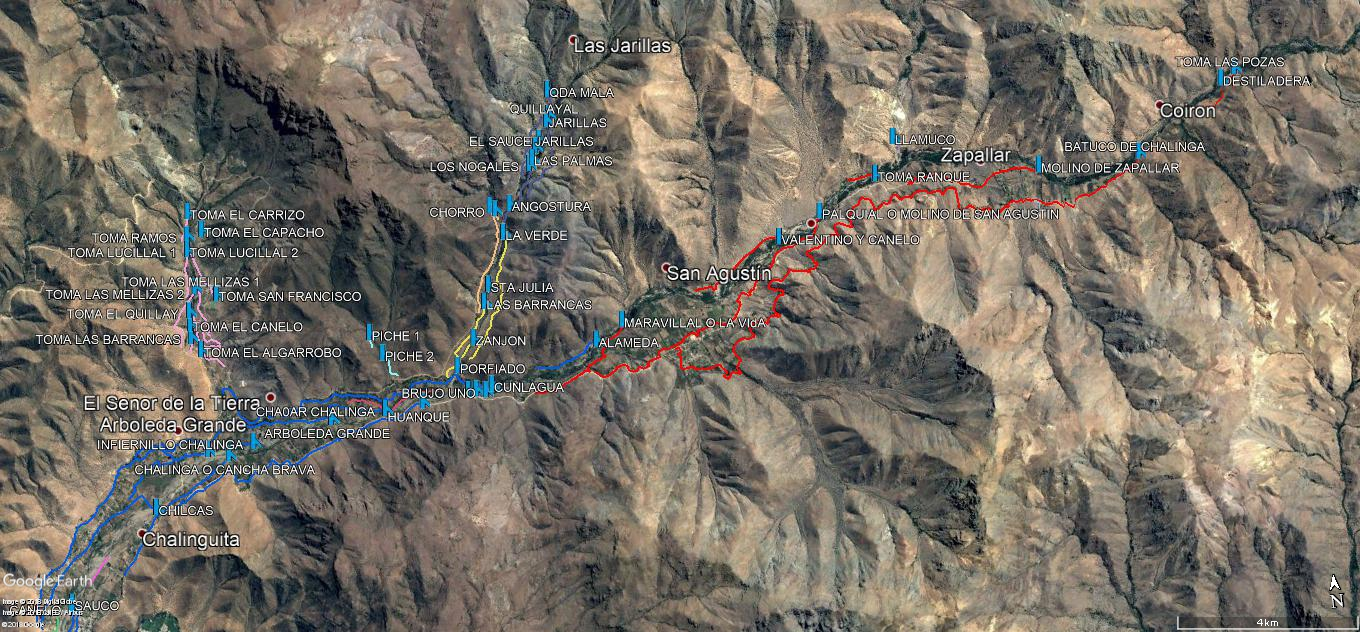
\includegraphics{SIG/canales.jpg}
	\caption{Capa canales y bocatomas de la Junta de Vigilancia Río Chalinga y sus afluentes (Fuente:CNR-DGA).}
	\label{canales}
\end{figure}

La recopilación de información de la OUA's, se realizó mediante la entrevista a un representante de la Junta de Vigilancia Río Chalinga y sus afluentes (ver anexo \ref{Entrevista OUA's}). Los antecedentes recopilados muestran que el número de total de acciones es de 5.500,33, las que equivalen a 2.376,76 $l/s$, distribuidas en 52 Comunidades de aguas con 1587 usuarios aproximadamente, donde 4 de ellas pertenecientes a la segunda sección del río Chalinga se encuentran sin información, por lo que estos resultados podrían variar, pero según señala la organización representan derechos eventuales atribuibles a usuarios exclusivos para cada una, los cuales no reciben aguas de forma constante (ver anexo \ref{canales chalinga}). No existe una relación lineal entre las acciones y los $l/s$ otorgados, llegando incluso a relaciones de 1/10 en algunas Comunidades de aguas, especialmente en afluentes y tributarios. \\
\\
La administración del recurso hídrico en la organización se realiza de forma continua en las 2 secciones en que se divide el río Chalinga, ya que no posee reservorio o embalse para acumulación y regulación de este, ajustando de forma constante el desmarque o entregas de aguas de acuerdo a disponibilidad. Además, los afluentes y tributarios del río Chalinga, donde se ubican algunas Comunidades de aguas, dependen de la eventualidad del recurso para su uso. Bajo estas condiciones, en conjunto con la OUA's se determinó realizar las actividades del protocolo en la primera y segunda sección del río Chalinga, sobre los canales que poseen acciones permanentes, y que por lo tanto, reciben aguas de forma constante. \\
\\
En la primera y segunda sección del río Chalinga, se encuentra aproximadamente el 80\% de los usuarios de aguas, es decir 1.284, los que representan un total de 1.673,23 acciones, equivalentes a 1.891,76 $l/s$, ocupando un 80\% de los $l/s$ totales de la organización. Se logró recopilar información de las siguientes variables de priorización para 17 canales (Cuadro \ref{priorización1}), junto con información para el desarrollo de actividades posteriores. En la primera sección, se decidió incorporar el canal Toma Las Pozas en el levantamiento de infromación, debido a que este es utilizado por la organización como reservorio para epocas de escasez. En la segunda sección, se decidió eliminar los canales Brujo n° cuatro infiernillo, Brujo n° Tres, Sauco y Canelo, debido a que presentan derechos eventuales y no reciben agua de forma constante, y además son de uso exclusivo por lo que no cumplen con las condiciones mínimas para desarrollar el protocolo. 

\begin{table}[H]
\centering
\caption{Comunidades de aguas Junta de Vigilancia Río Chalinga y sus afluentes incluídas en el Protocolo.}
\label{priorización1}
	\begin{tabular}{|c|l|c|c|c|}
	\hline
	\textbf{N°} & \textbf{Comunidad de Aguas o Canal} & \textbf{Acciones} & \textbf{Capacidad de} & \textbf{Número de} \\
	& & & \textbf{porteo ($l/s$)} & \textbf{beneficiarios} \\ \hline
	1 & Batuco de Chalinga 					& 205,08 & 330 	 & 153	\\ \hline
	2 & Molino de Zapallar 					& 59 	 & 100 	 & 18 	\\ \hline
	3 & Palquial o Molino de San Agustín	& 245,2	 & 319 	 & 55 	\\ \hline
	4 & Valentino o Canelo					& 18,2 	 & 25	 & 2 	\\ \hline
	5 & Maravillal o La Viña				& 26,3	 & 50	 & 9 	\\ \hline
	6 & Alameda Derecha						& 27,4	 & 70 	 & 15 	\\ \hline
	7 & Gavino								& 30	 & 33 	 & 43 	\\ \hline
	8 & Destiladera							& 100 	 & 150 	 & 43 	\\ \hline
	9 & Ranque								& 12 	 & 40 	 & 10 	\\ \hline
	10 & Cunlagua							& 116,1	 & 250 	 & 136 	\\ \hline
	11 & Huanque							& 109,26 & 140 	 & 97 	\\ \hline
	12 & Chañar	Chalinga					& 40,26	 & 55	 & 26 	\\ \hline
	13 & Arboleda Grande					& 104,93 & 165 	 & 160 	\\ \hline
	14 & El Tebal							& 172 	 & 100	 & 259 	\\ \hline
	15 & Chalinga o Cancha Brava			& 98,78	 & 130,9 & 85 	\\ \hline
	16 & Chilcas							& 74	 & 132 	 & 102 	\\ \hline
	17 & Los Guindos						& 224 	 & 30,8  & 28 	\\ \hline	
	\end{tabular}
\end{table}

La información recopilada de las Comunidades de aguas, se efectuó a través de la entrevista a un representante de esta, donde se validó la información obtenida en la OUA's y se completó la información de capacidad de porteo, la cual no se disponía en la organización (ver anexo \ref{Entrevista CA's}. Para los casos en que la capacidad de porteo no fue posible obtener, debido a desconocimiento principalmente, se optó por realizar un estimativo aumentando en un 10\% su capacidad máxima en $l/s$. Además, se logró generar el contacto con estos para el apoyo en el S.I.G. del canal, otorgando información valiosa del trazado del canal matriz y ubicación de ramales o derivados principalmente.

\clearpage
\subsection{Componente 2. Actividad 2.6. Plan de Priorización de canales y/o tramos de la red de distribución de la Junta de Vigilancia Río Chalinga y sus afluentes.}


\subsection{Componente 1. Actividad 1.4. Validación del protocolo técnico-social de inversión en mejoramiento de la eficiencia de conducción hídrica.}

Se seleccionaron tres Comunidades de aguas, denominadas Chalinga o Cancha Brava, Arboleda Grande y Huanque, las que se encuentran bajo la jurisdicción de la Junta de Vigilancia Río Chalinga y sus Afluentes, en la cuenca del río Chalinga. Se enfocará en esta cuenca con el fin de avanzar en la creación del primer Plan de priorización para la OUA's comprometido.

\subsubsection{Recopilación de información.}

\begin{itemize}
	\item[$-$] \textbf{Recopilación bibliográfica cuenca río Chalinga}
\end{itemize}

Como primera información, se recopiló la ficha de registros de bocatomas, generada por la Dirección General de Aguas, junto con la información geoespacial denominada Canales de riego a nivel matrices hasta 2do derivado de la Comisión Nacional de Riego. Además estos antecedentes no permitirán apoyarnos en el levantamiento del S.I.G. y determinación de superficies bajo riego y superficie potencial.

\begin{itemize}
	\item[$-$] \textbf{Información Junta de Vigilancia Río Chalinga y sus Afluentes}
\end{itemize}

A través de mesas de trabajo conformadas por el equipo del proyecto y la organización, se recopiló la siguiente información:

\begin{itemize}	
	\item Diagrama unifilar: Recopilación de archivos en formato pdf.
	\item Ubicación geográfica bocatomas: Apoyo para ubicación de bocatomas con el Sr. Wenceslao Layana, Asesor Técnico.
	\item Número de acciones totales: Revisión de archivos, recopilado mediante digitalización.
	\item Número de acciones por comunidad de aguas: Revisión de archivos, recopilado mediante digitalización.
	\item Dotaciones o desmarques: Revisión de archivos, recopilado mediante digitalización.
	\item Capacidad de porteo de cada canal: Información no disponible, se estableció un 10\% extra de la entrega total en $l/s$.
	\item Número de usuarios comunidad de aguas: Recopilación de archivos actualizados por el programa de fortalecimiento de la CNR en ejecución en la organización.
	\item Superficie regada por comunidad de aguas: Revisión de archivos, recopilado mediante digitalización.
	\item Contacto celadores: Se realiza en forma constante con el Sr. Wenceslao Layana, Asesor Técnico de la OUA's.
\end{itemize}
\clearpage
\begin{itemize}
	\item[$-$] \textbf{Información Comunidad de Aguas Chalinga o Cancha Brava}
\end{itemize}

Se realizó la entrevista a un representante de la Comunidad de aguas, los antecedentes recolectados se presentan a continuación:

\begin{figure} [H]
	\fbox{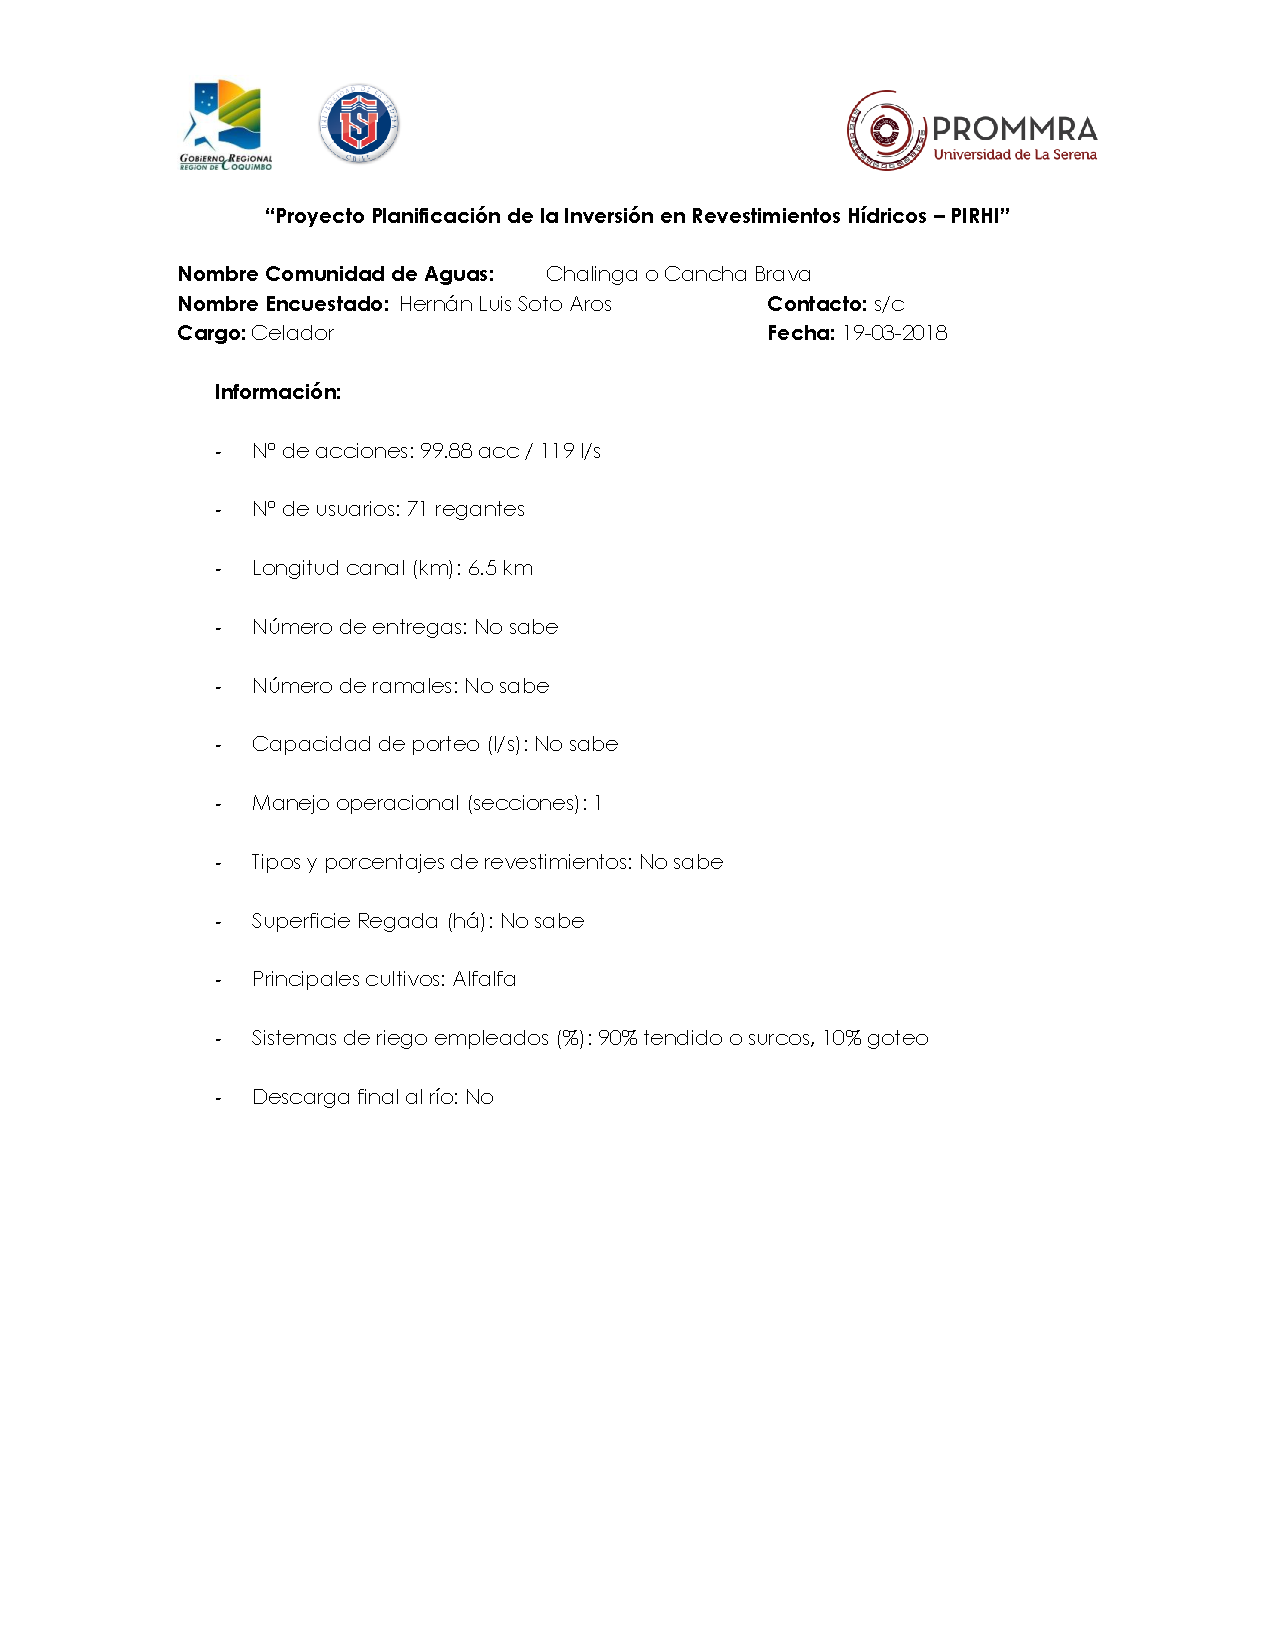
\includegraphics[height=19cm]{EntrevistasCA/Chalinga.pdf}}
	\caption{Entrevista Comunidad de aguas Chalinga o Cancha Brava.}
\end{figure}
\clearpage
\begin{itemize}
	\item[$-$] \textbf{Información Comunidad de Aguas Arboleda Grande}
\end{itemize}

Se realizó la entrevista a un representante de la Comunidad de aguas, los antecedentes recolectados se presentan a continuación:

\begin{figure} [H]
  \fbox{\includegraphics[height=19cm]{EntrevistasCA/Arboleda_grande.pdf}}
	\caption{Entrevista Comunidad de aguas Arboleda grande.}
\end{figure}
\clearpage
\begin{itemize}
	\item[$-$] \textbf{Información Comunidad de Aguas Huanque}
\end{itemize}

Se realizó la entrevista a un representante de la Comunidad de aguas, los antecedentes recolectados se presentan a continuación:

\begin{figure} [H]
  \fbox{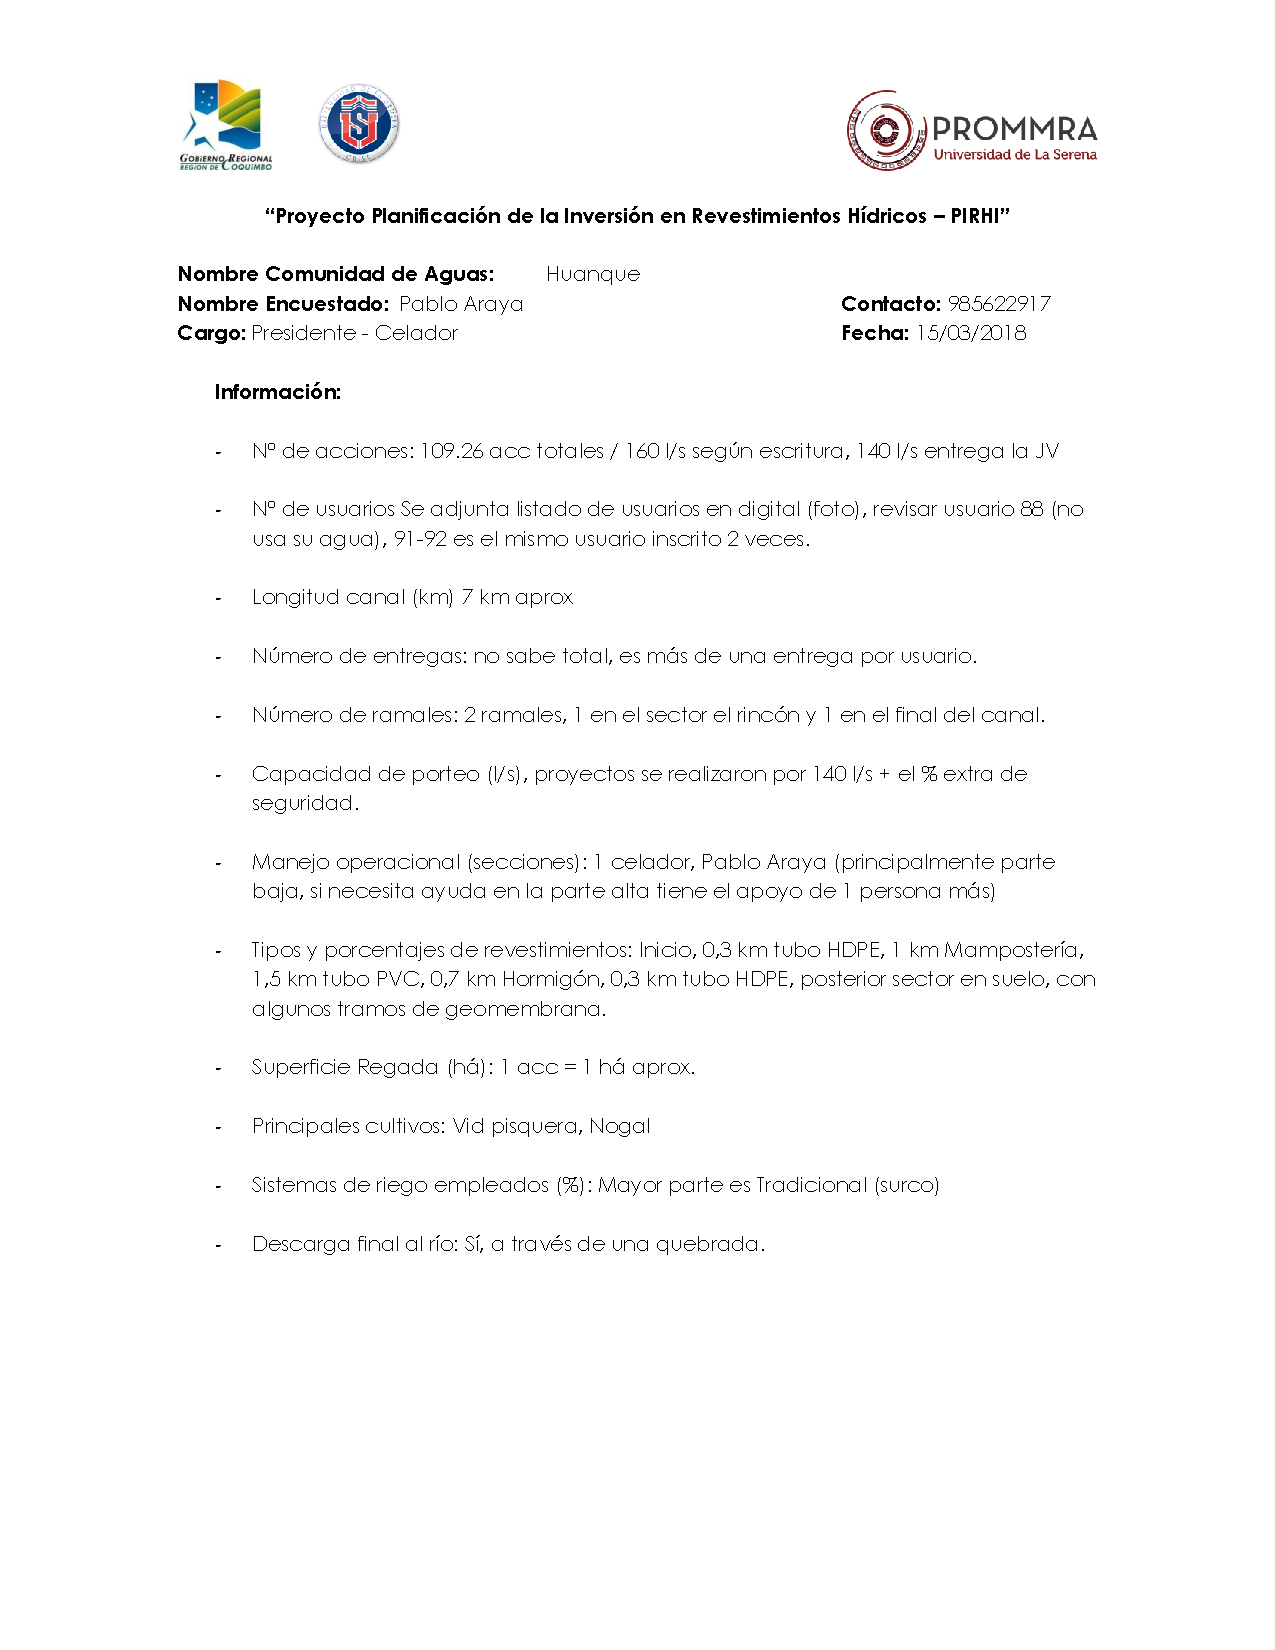
\includegraphics[height=19cm]{EntrevistasCA/Huanque.pdf}}
	\caption{Entrevista Comunidad de aguas Huanque.}
\end{figure}
\clearpage
Como resultado de la recopilación de información a nivel de cuenca, OUA's y Comunidades de aguas, se pudo obtener la siguientes información:

\begin{table}[H]
\caption{Variables obtenidas de la recopilación de Información}
\begin{tabular}{l|c|c|c|}
\cline{2-4}
  & \multicolumn{3}{c|}{\textbf{Comunidades de Aguas o canal}                                                          } \\ \hline
\multicolumn{1}{|c|}{\textbf{\begin{tabular}[c]{@{}c@{}}Variable \\\end{tabular}}} & \textbf{Arboleda Grande} & \textbf{Chalinga o Cancha Brava} & \textbf{Huanque}         \\ \hline
\multicolumn{1}{|l|}{\textbf{Número de acciones}}       & 98,78 & 104,93 & 109,26\\
\multicolumn{1}{|l|}{\textbf{Capacidad de porteo ($l/s$)}}        &   129,9   &     165     &  154 \\
\multicolumn{1}{|l|}{\textbf{Número de beneficiarios}}        & 85 & 160 & 97\\ \hline
\end{tabular}
\end{table}

\subsubsection{Sistema de Información Geográfica (S.I.G.).}

En una primera campaña de terreno, realizada en el mes de Marzo, se realizaron por completo la georeferenciación de 3 canales correspondiente al área de la Junta de Vigilancia del Río Chalinga y sus Afluentes. Se llevo a cabo en 3 canales de la segunda sección del río Chalinga, la cual posee la mayor longitud en la red de canales con 41,62 km (según capa canales CNR), por la operatividad y disponibilidad de personal de las comunidades de agua que conforman el área de Chalinga, las comunidades de aguas Arboleda Grande, Chalinga o Cancha Brava y Huanque, representan el 12,5\%, 8,8\% y 16,7\% de la longitud total de la red de la segunda sección del río respectivamente según los datos obtenidos de CNR.\\
\\
Mediante GPS diferencial y el diccionario incorporado a estos, se logró georeferenciar y describir cada uno de las obras a levantar en el recorrido de los canales. A modo de resumen se presenta la información recabada en las bocatoma de estos canales.

\begin{table}[H]
\caption{Descripción Bocatomas}
\label{my-label}
\begin{tabular}{l|c|c|c|}
\cline{2-4}
                                                                                              & \multicolumn{3}{c|}{\textbf{Canales}                                                          } \\ \hline
\multicolumn{1}{|c|}{\textbf{\begin{tabular}[c]{@{}c@{}}Componente \\ Bocatoma\end{tabular}}} & \textbf{Arboleda Grande} & \textbf{Chalinga o Cancha Brava} & \textbf{Huanque}         \\ \hline
\multicolumn{1}{|l|}{\textbf{Obra desviación}}                                               & Barrera lateral          & Compuerta hoja metálica          & Barrera lateral          \\
\multicolumn{1}{|l|}{\textbf{Canal aducción}}                                                 & 867,45 m                 & 568,18 m                         & 184,73 m                 \\
\multicolumn{1}{|l|}{\textbf{Compuerta Carga}}                                                & Compuerta manual & Compuerta manual         & Compuerta manual \\
\multicolumn{1}{|l|}{\textbf{Sección Control}}                                                & Aforador Parshall        & Aforador Parshall                & Aforador Parshall        \\ \hline
\end{tabular}
\end{table}

La caracterización realizada a nivel de canal presenta información como longitud y tipos de revestimientos, estructuras de distribución y puntos críticos. Además esta información nos permitirá definir los tramos para evaluación de pérdidas por conducción, proporcionar las dimensiones de la sección afecta a revestimiento, validar o ajustar el trazado del canal que en primera instancia se obtuvo de la capa de la CNR, y así rectificar las superficies asociadas a cada canal, las cuales fueron asignadas en base la capa CNR.\\
\\ 
Para la definición de la longitud que utiliza el protocolo, se recolectó las coordenadas, revestimiento (número de paredes del canal revestida), tipo de revestimiento (permanente o temporal) y material de revestimiento en cada cambio de revestimiento, lo que permite dar cumplimiento para la definición de estas longitudes.\\
\\
A continuación se presenta un resumen de longitudes que presentan los 3 canales validados.

\begin{table}[H]
\centering
\caption{Longitudes por canal}
\label{my-label}
\resizebox{\textwidth}{!}{%
\begin{tabular}{|l|c|c|c|}
\hline
\textbf{Canal}           & \textbf{Canal aducción ($km$)} & \textbf{Canal conducción y distribución ($km$)} & \textbf{Total General ($km$)} \\ \hline
\textbf{Arboleda Grande} & 0,87  & 5,03 & 5,90   \\ \hline
\textbf{Cancha Brava}    & 0,57  & 3,84 & 4,41 \\ \hline
\textbf{Huanque}        & 0,18  & 7,01   & 7,19 \\ \hline
\end{tabular}%
}
\end{table}

Para las estructuras de distribución mediante la captura de sus coordenadas y caracterización del tipo de obra, se obtiene el requerimiento que permitirá definir tramo matriz y puntos de entrega tomándose en cuenta para la evaluación de pérdidas. \\
\\
En la validación se obtiene que los canales presentan los siguientes estructuras de distribución.

\begin{table}[H]
\centering
\caption{Estructuras de distribución}
\label{my-label}
\begin{tabular}{l|c|c|c|c}
\cline{2-4}
                                                       & \multicolumn{3}{c|}{\textbf{Estructura distribución}} & \multicolumn{1}{l}{}                        \\ \hline
\multicolumn{1}{|l|}{\textbf{Canal}}                   & \textbf{Entrega}  & \textbf{Gestión} & \textbf{Ramal} & \multicolumn{1}{c|}{\textbf{Total general}} \\ \hline
\multicolumn{1}{|l|}{\textbf{Arboleda Grande}}         & 88                & 32               & 7              & \multicolumn{1}{c|}{127}                    \\ \hline
\multicolumn{1}{|l|}{\textbf{Chalinga o Cancha Brava}} & 68                & 53               & 5              & \multicolumn{1}{c|}{126}                    \\ \hline
\multicolumn{1}{|l|}{\textbf{Huanque}}                 & 100               & 56               & 3              & \multicolumn{1}{c|}{159}                    \\ \hline
\end{tabular}
\end{table}

Dentro de las estructuras de distribución se agrega la función de ramal, la cual no se consideraba para el protocolo del proyecto SIMCA-Elqui, esta función busca conocer donde nacen los derivados y estimar superficie irrigada por el ramal, ajustando la asignación de la superficie a los canales si se encuentra más de un canal cercano en el territorio.\\
\\
En el recorrido de canal se obtuvieron coordenadas de inicio, fin y algunos puntos críticos que se presenten en el canal, como filtraciones, quebradas, desbordes, entre otros, que puedan afectar la conducción y distribución normal del recurso, por lo cual dependiendo del tipo de observación y longitud de este hito se definirá si es necesario realizar un subtramo adicional para evaluación de pérdidas los cuales son definidos por los cambios de revestimientos.\\
\\
Los resultados obtenidos para la validación de variables que contemple el protocolo como insumos para priorización con se presentan a continuación: 

% Please add the following required packages to your document preamble:
% \usepackage{graphicx}
\begin{table}[H]
\caption{Resultados variables longitudes y dimensiones}
\begin{tabular}{|l|ccc|}
\hline
\textbf{Variables}  & \textbf{Arboleda Grande} & \textbf{Chalinga o} & \textbf{Huanque} \\
 & & \textbf{Cancha Brava} &  \\ \hline                          
\textbf{Longitud total de canal en uso ($km$)}   & 5.902    & 4.406    & 7.190  \\
\textbf{Longitud tramo matriz ($km$)}  & 0.046    & 0.045    & 0.071    \\
\textbf{Longitud Tramo conducción ($km$)}  & 4.989  & 3.792  & 6.934   \\
\textbf{Longitud afecta a mejoramiento ($km$)}   & 2.149     & 2.306   & 2.472  \\
\textbf{*Dimensiones a revestir  (ancho; alto) ($m$)} & 0,6; 0,5 & 0,9; 0,7 & 0,5; 0,4\\ 
\hline
\end{tabular}
\small{*Sección rectangular revestida en hormigón}\\
\end{table}

\subsubsection{Determinación general de pérdidas.}

La información del S.I.G. nos permite generar los tramos de aforo para la determinación de pérdidas, basado en la primera entrega para definir el tramo matriz (se presentan los datos en color rojo) y tipos de revestimientos presentes. A continuación se presentan los tramos generados para cada Comunidad de aguas.

\begin{itemize}
	\item[$-$] \textbf{Comunidad de Aguas Chalinga o Cancha Brava}
\end{itemize}

\begin{table}[H]
\centering
\caption{Tramos del canal Chalinga o Cancha Brava.}
\label{matriz}
\begin{tabular}{|c|c|c|c|c|c|c|c|}
\hline
\textbf{Tramo} & \textbf{\begin{tabular}[c]{@{}c@{}}N°\\ aforo \\ inicial\end{tabular}} & \textbf{\begin{tabular}[c]{@{}c@{}}N°\\ aforo\\ final\end{tabular}} & \textbf{\begin{tabular}[c]{@{}c@{}}Km\\ inicial\end{tabular}} & \textbf{\begin{tabular}[c]{@{}c@{}}Km\\ final\end{tabular}} & \textbf{\begin{tabular}[c]{@{}c@{}}Longitud\\ ($km$)\end{tabular}} & \textbf{Revestimiento}   & \textbf{Hitos} \\ \hline                                                                                   
{\color[HTML]{FE0000} \textbf{1}} & {\color[HTML]{FE0000} \textbf{1}} & {\color[HTML]{FE0000} \textbf{2}} & {\color[HTML]{FE0000} \textbf{0,00}}& {\color[HTML]{FE0000} \textbf{0,04}} & {\color[HTML]{FE0000} \textbf{0,04}} & {\color[HTML]{FE0000} \textbf{Hormigón}} & {\color[HTML]{FE0000} \textbf{Sección Matriz}} \\ \hline
\textbf{2} & 2 & 20 & 0,04 & 1,37 & 1,33 & Hormigón & - \\ \hline
\textbf{3} & 20 & 23 & 1,37 & 1,70 & 0,33 & Geomembrana & - \\ \hline
\textbf{4} & 23 & 26 & 1,70 & 1,80 & 0,10 & \begin{tabular}[c]{@{}c@{}}Hormigón - \\ Loseta\end{tabular} & - \\ \hline                                                                                             
\textbf{5} & 26 & 73 & 1,80 & 3,84 & 2,04 & Geomembrana & - \\ \hline                                                                                      
\end{tabular}
\end{table}

El trazado del canal Chalinga o Cancha Brava se encuentra revestido en su totalidad, donde se presentan revestimientos de tipo permanente y temporal. Este se dividió en 5 tramos, los que se desglosan en el tramo matriz y 4 tramos de distribución. El tramo matriz o 1, junto a los tramos de distribución 2 y 4, presentan revestimientos de tipo permanente, cuyo material principal es hormigón. Los tramos 3 y 5, corresponde a geomembrana, la cual es de tipo temporal y poseen en conjunto una longitud de 2,37 $km$.

\begin{itemize}
	\item[$-$] \textbf{Comunidad de Aguas Arboleda Grande.}
\end{itemize}

\begin{table}[H]
\centering
\caption{Tramos del canal Arboleda Grande.}
\label{matriz}
\begin{tabular}{|c|c|c|c|c|c|c|c|}
\hline
\textbf{Tramo} & \textbf{\begin{tabular}[c]{@{}c@{}}N°\\ aforo \\ inicial\end{tabular}} & \textbf{\begin{tabular}[c]{@{}c@{}}N°\\ aforo\\ final\end{tabular}} & \textbf{\begin{tabular}[c]{@{}c@{}}Km\\ inicial\end{tabular}} & \textbf{\begin{tabular}[c]{@{}c@{}}Km\\ final\end{tabular}} & \textbf{\begin{tabular}[c]{@{}c@{}}Longitud\\ ($km$)\end{tabular}} & \textbf{Revestimiento}   & \textbf{Hitos} \\ \hline                                                                                   
{\color[HTML]{FE0000} \textbf{1}} & {\color[HTML]{FE0000} \textbf{1}} & {\color[HTML]{FE0000} \textbf{2}} & {\color[HTML]{FE0000} \textbf{0,00}}& {\color[HTML]{FE0000} \textbf{0,05}} & {\color[HTML]{FE0000} \textbf{0,05}} & {\color[HTML]{FE0000} \textbf{Mezcla suelo}} & {\color[HTML]{FE0000} \textbf{Sección Matriz}} \\ \hline
\textbf{2} & 2 & 7 & 0,05 & 0,34 & 0,29 & Mezcla suelo & - \\ \hline
\textbf{3} & 7 & 21 & 0,34 & 0,94 & 0,60 & Geomembrana & - \\ \hline
\textbf{4} & 21 & 45 & 0,94 & 2,18 & 1,24 & Loseta & - \\ \hline                                                                                             
\textbf{5} & 46 & 48 & 2,18 & 2,37 & 0,19 & \begin{tabular}[c]{@{}c@{}}Tubo PVC - \\ Tubo metálico\end{tabular} & - \\ \hline                                                                                      
\textbf{6} & 48 & 66 & 2,37 & 3,20 & 0,84 & Loseta & - \\ \hline
\textbf{7} & 66 & 79 & 3,20 & 3,77 & 0,57 & Hormigón & - \\ \hline                                                                                                                                                                            
\textbf{8} & 79 & 104 & 3,77 & 4,99 & 1,21 & Mezcla suelo & - \\ \hline                                                                                      
\textbf{9} & 104 & 105 & 4,99 & 5,03 & 0,05 & Tubo PVC & - \\ \hline                                                                                      
\end{tabular}
\end{table}

El trazado del canal se dividió en 9 tramos. La longitud total de los tramos a evaluar es de 5,03 $km$, de los cuales los primeros 0,6 $km$ corresponden a sin revestimiento o revestimiento temporal. Los siguientes 2,84 $km$, corresponden a revestimiento de tipo permanente, del cual se destaca el material de tipo loseta. La parte final del trazado se encuentra sin revestimiento en su mayoría, solo los últimos 0,05 $km$ se encuentran en tubo de PVC.
\clearpage
\begin{itemize}
	\item[$-$] \textbf{Comunidad de Aguas Huanque.}
\end{itemize}

\begin{table}[H]
\centering
\caption{Tramos del canal Huanque.}
\label{matriz}
\begin{tabular}{|c|c|c|c|c|c|c|c|}
\hline
\textbf{Tramo} & \textbf{\begin{tabular}[c]{@{}c@{}}N°\\ aforo \\ inicial\end{tabular}} & \textbf{\begin{tabular}[c]{@{}c@{}}N°\\ aforo\\ final\end{tabular}} & \textbf{\begin{tabular}[c]{@{}c@{}}Km\\ inicial\end{tabular}} & \textbf{\begin{tabular}[c]{@{}c@{}}Km\\ final\end{tabular}} & \textbf{\begin{tabular}[c]{@{}c@{}}Longitud\\ ($km$)\end{tabular}} & \textbf{Revestimiento}   & \textbf{Hitos} \\ \hline                                                                                   
{\color[HTML]{FE0000} \textbf{1}} & {\color[HTML]{FE0000} \textbf{1}} & {\color[HTML]{FE0000} \textbf{2}} & {\color[HTML]{FE0000} \textbf{0,00}}& {\color[HTML]{FE0000} \textbf{0,02}} & {\color[HTML]{FE0000} \textbf{0,02}} & {\color[HTML]{FE0000} \textbf{Hormigón Roca}} & {\color[HTML]{FE0000} \textbf{Sección Matriz}} \\ \hline
{\color[HTML]{FE0000} \textbf{2}} & {\color[HTML]{FE0000} \textbf{2}} & {\color[HTML]{FE0000} \textbf{3}} & {\color[HTML]{FE0000} \textbf{0,02}}& {\color[HTML]{FE0000} \textbf{0,07}} & {\color[HTML]{FE0000} \textbf{0,05}} & {\color[HTML]{FE0000} \textbf{Tubo HDPE}} & {\color[HTML]{FE0000} \textbf{\begin{tabular}[c]{@{}c@{}}Término sección\\ Matriz\end{tabular}}} \\ \hline
\textbf{3} & 3 & 5 & 0,07 & 0,46 & 0,39 & Tubo HDPE & - \\ \hline
\textbf{4} & 5 & 19 & 0,46 & 1,49 & 1,03 & Hormigón Roca & - \\ \hline                                                                                             
\textbf{5} & 19 & 52 & 1,49 & 3,40 & 1,91 & Tubo PVC & - \\ \hline                                                                                      
\textbf{6} & 52 & 56 & 3,40 & 4,04 & 4,53 & Hormigón & - \\ \hline
\textbf{7} & 56 & 64 & 4,04 & 4,53 & 0,50 & Tubo HDPE & - \\ \hline                                                                                                                                                                            
\textbf{8} & 64 & 71 & 4,53 & 4,76 & 0,22 & Mezcla suelo & - \\ \hline                                                                                      
\textbf{9} & 71 & 96 & 4,76 & 5,70 & 0,95 & Geomembrana & - \\ \hline                                                                                      
\textbf{10} & 96 & 110 & 5,70 & 6,14 & 0,44 & Mezcla suelo & - \\ \hline
\textbf{11} & 110& 113 & 6,14 & 6,83 & 0,68 & Geomembrana & - \\ \hline
\textbf{12} & 113 & 119 & 6,83 & 7,01 & 0,18 & Mezcla suelo & - \\ \hline
\end{tabular}
\end{table}

Para el canal Huanque se generó un total de 12 tramos, de los cuales los 2 primeros corresponden a canal matriz, debido al cambio de revestimiento presente. Hasta el 4,53 $km$ de recorrido se presentan revestimientos de tipo permanente, mientras que los 2,48 $km$ restantes no presentan revestimiento o corresponde a tipo temporal.

La campaña de aforos se desarrollo en el mes de Abril. Al realizar los aforos de inicio y fin de cada tramo, se procedió a realizar la evaluación de pérdidas para una posible subdivisión. Los resultados se presentan a continuación.

\clearpage
\begin{landscape}
\begin{itemize}
	\item[$-$] \textbf{Comunidad de Aguas Chalinga o Cancha Brava.}
\end{itemize}

\begin{table}[H]
\centering
\caption{Tramos aforados del canal Chalinga o Cancha Brava.}
\label{matriz}
\resizebox{23cm}{!} {
\begin{tabular}{|c|c|c|c|c|c|c|c|c|c|c|c|c|c|}
\hline
\textbf{Tramo} & \textbf{\begin{tabular}[c]{@{}c@{}}N°\\ aforo \\ inicial\end{tabular}} & \textbf{\begin{tabular}[c]{@{}c@{}}N°\\ aforo\\ final\end{tabular}} & \textbf{\begin{tabular}[c]{@{}c@{}}Km\\ inicial\end{tabular}} & \textbf{\begin{tabular}[c]{@{}c@{}}Km\\ final\end{tabular}} & \textbf{\begin{tabular}[c]{@{}c@{}}Longitud\\ ($km$)\end{tabular}} & \textbf{\begin{tabular}[c]{@{}c@{}}Q Inicial\\ ($l/s$)\end{tabular}}   & \textbf{\begin{tabular}[c]{@{}c@{}}Q Final\\ Real ($l/s$)\end{tabular}} & \textbf{\begin{tabular}[c]{@{}c@{}}Q Antes\\ Entrega o\\ Aporte ($l/s$)\end{tabular}} & \textbf{\begin{tabular}[c]{@{}c@{}}Q Después\\ Entrega o\\ Aporte ($l/s$)\end{tabular}} & \textbf{\begin{tabular}[c]{@{}c@{}}Q  Entrega o\\ Aporte ($l/s$)\end{tabular}} & \textbf{\begin{tabular}[c]{@{}c@{}}Q  Final\\ Teórico ($l/s$)\end{tabular}} & \textbf{\begin{tabular}[c]{@{}c@{}}Pérdidas\\ ($l/s$)\end{tabular}} & \textbf{\begin{tabular}[c]{@{}c@{}}Pérdidas\\ ($\%$)\end{tabular}} \\ \hline                                                                                   
{\color[HTML]{FE0000} \textbf{1}} & {\color[HTML]{FE0000} \textbf{1}} & {\color[HTML]{FE0000} \textbf{2}} & {\color[HTML]{FE0000} \textbf{0,00}}& {\color[HTML]{FE0000} \textbf{0,04}} & {\color[HTML]{FE0000} \textbf{0,04}} & {\color[HTML]{FE0000} \textbf{54,07}} & {\color[HTML]{FE0000} \textbf{54,07}} & & & & {\color[HTML]{FE0000} \textbf{54,07}} & {\color[HTML]{FE0000} \textbf{0,00}} & {\color[HTML]{FE0000} \textbf{0,00}} \\ \hline
\textbf{2} & 2 & 20 & 0,04 & 1,37 & 1,33 & 54,07 & 51,30 & & & & 51,30 & 2,77 & 5,12 \\ \hline
\textbf{3} & 20 & 23 & 1,37 & 1,70 & 0,33 & 51,30 & 35,35 & & & & 35,35 & 15,95 & 31,09 \\ \hline
\textbf{4} & 23 & 26 & 1,70 & 1,80 & 0,10 & 35,35 & 35,35 & & & & 35,35 & 0,00 & 0,00 \\ \hline                                                                                             
\textbf{5.1} & 26 & 46 & 1,80 & 2,89 & 1,09 & 35,35 & 34,22 & & & & 34,22 & 1,13 & 3,20 \\ \hline                                                                                      
\textbf{5.2} & 46 & 73 & 2,89 & 3,84 & 0,94 & 34,22 & 22,41 & & & & 22,41 & 11,81 & 34,51 \\ \hline                                                                                      
\end{tabular}
}
\end{table}

La determinación de pérdidas por tramos del canal Chalinga o Cancha Brava, muestra que la mayor pérdida por conducción se produce en los tramos 3 y 5, en donde este último generó 2 subtramos debido a su alta pérdida. El tramo 3 presenta un 31,09$\%$ de pérdidas, donde se puedo apreciar el mal estado de la geomembrana presente y una alta concentración de vegetación. El subtramo 5.2, correspondiente al trazado final del canal, presenta una pérdida del 34,51$\%$, con un revestimiento de tipo temporal, convirtiéndose en el sector con mayores pérdidas, lo que puede deberse a la mala instalación de la geomembrana en algunos sectores. Los tramos restantes presentan pérdidas menores al 6$\%$. 

\begin{table}[H]
\centering
\caption{Pérdidas generales del canal Chalinga o Cancha Brava.}
\label{matriz}
\resizebox{23cm}{!} {
\begin{tabular}{|c|c|c|c|c|c|c|c|c|c|c|}
\hline
\textbf{Tramo} & \textbf{\begin{tabular}[c]{@{}c@{}}Q Inicial\\ ($l/s$)\end{tabular}}   & \textbf{\begin{tabular}[c]{@{}c@{}}Q Final\\ Real ($l/s$)\end{tabular}} & \textbf{\begin{tabular}[c]{@{}c@{}}Q Antes\\ Entrega o\\ Aporte ($l/s$)\end{tabular}} & \textbf{\begin{tabular}[c]{@{}c@{}}Q Después\\ Entrega o\\ Aporte ($l/s$)\end{tabular}} & \textbf{\begin{tabular}[c]{@{}c@{}}Q  Entrega o\\ Aporte ($l/s$)\end{tabular}} & \textbf{\begin{tabular}[c]{@{}c@{}}Q  Final\\ Teórico ($l/s$)\end{tabular}} & \textbf{\begin{tabular}[c]{@{}c@{}}Pérdidas\\ ($l/s$)\end{tabular}} & \textbf{\begin{tabular}[c]{@{}c@{}}Pérdidas\\ ($\%$)\end{tabular}} & \textbf{\begin{tabular}[c]{@{}c@{}}Pérdidas\\ ($l/km$)\end{tabular}} & \textbf{\begin{tabular}[c]{@{}c@{}}Pérdidas\\ ($\%/km$)\end{tabular}} \\ \hline                                                                                   
{\color[HTML]{FE0000} \textbf{1}} & {\color[HTML]{FE0000} \textbf{54,07}} & {\color[HTML]{FE0000} \textbf{54,07}} & & & & {\color[HTML]{FE0000} \textbf{54,07}} & {\color[HTML]{FE0000} \textbf{0,00}} & {\color[HTML]{FE0000} \textbf{0,00}} & {\color[HTML]{FE0000} \textbf{0,00}}  &  {\color[HTML]{FE0000} \textbf{0,00}}  \\ \hline
\textbf{2} & 54,07 & 51,30 & & & & 51,30 & 2,77 & 5,12 & 2,09 & 3,86  \\ \hline
\textbf{3} & 51,30 & 35,35 & & & & 35,35 & 15,95 & 31,09 & 48,48 & 94,51  \\ \hline
\textbf{4} & 35,35 & 35,35 & & & & 35,35 & 0,00 & 0,00 & 0,00 & 0,00   \\ \hline
\textbf{5.1} & 35,35 & 34,22 & & & & 34,22 & 1,13 & 3,20 & 1,03 & 2,92  \\ \hline
\textbf{5.2} & 34,22 & 22,41 & & & & 22,41 & 11,81 & 34,51 & 12,51 & 36,55 \\ \hline     
\end{tabular}
}
\end{table}

Al analizar la pérdida general del tramo 3 en $\%/km$, se lográ establecer una pérdida de 94,51$\%/km$, por lo que este tramo permitiría una gran recuperación de ser mejorado. 

\clearpage
\begin{itemize}
	\item[$-$] \textbf{Comunidad de Aguas Arboleda Grande.}
\end{itemize}

\begin{table}[H]
\centering
\caption{Tramos del canal Arboleda Grande.}
\label{matriz}
\resizebox{23cm}{!} {
\begin{tabular}{|c|c|c|c|c|c|c|c|c|c|c|c|c|c|}
\hline
\textbf{Tramo} & \textbf{\begin{tabular}[c]{@{}c@{}}N°\\ aforo \\ inicial\end{tabular}} & \textbf{\begin{tabular}[c]{@{}c@{}}N°\\ aforo\\ final\end{tabular}} & \textbf{\begin{tabular}[c]{@{}c@{}}Km\\ inicial\end{tabular}} & \textbf{\begin{tabular}[c]{@{}c@{}}Km\\ final\end{tabular}} & \textbf{\begin{tabular}[c]{@{}c@{}}Longitud\\ ($km$)\end{tabular}} & \textbf{\begin{tabular}[c]{@{}c@{}}Q Inicial\\ ($l/s$)\end{tabular}}   & \textbf{\begin{tabular}[c]{@{}c@{}}Q Final\\ Real ($l/s$)\end{tabular}} & \textbf{\begin{tabular}[c]{@{}c@{}}Q Antes\\ Entrega o\\ Aporte ($l/s$)\end{tabular}} & \textbf{\begin{tabular}[c]{@{}c@{}}Q Después\\ Entrega o\\ Aporte ($l/s$)\end{tabular}} & \textbf{\begin{tabular}[c]{@{}c@{}}Q  Entrega o\\ Aporte ($l/s$)\end{tabular}} & \textbf{\begin{tabular}[c]{@{}c@{}}Q  Final\\ Teórico ($l/s$)\end{tabular}} & \textbf{\begin{tabular}[c]{@{}c@{}}Pérdidas\\ ($l/s$)\end{tabular}} & \textbf{\begin{tabular}[c]{@{}c@{}}Pérdidas\\ ($\%$)\end{tabular}} \\ \hline 
{\color[HTML]{FE0000} \textbf{1}} & {\color[HTML]{FE0000} \textbf{1}} & {\color[HTML]{FE0000} \textbf{2}} & {\color[HTML]{FE0000} \textbf{0,00}}& {\color[HTML]{FE0000} \textbf{0,05}} & {\color[HTML]{FE0000} \textbf{0,05}} & {\color[HTML]{FE0000} \textbf{58,20}} & {\color[HTML]{FE0000} \textbf{58,20}} & & & & {\color[HTML]{FE0000} \textbf{58,20}} & {\color[HTML]{FE0000} \textbf{0,00}} & {\color[HTML]{FE0000} \textbf{0,00}} \\ \hline
\textbf{2} & 2 & 7 & 0,05 & 0,34 & 0,29 & 58,20 & 44,70 & & & & 44,70 & 13,50 & 23,20 \\ \hline
\textbf{3} & 7 & 21 & 0,34 & 0,94 & 0,60 & 44,70 & 16,00 & 42,90 & 18,3 & 24,60 & 40,60 & 4,10 & 9,17 \\ \hline
\textbf{4} & 21 & 45 & 0,94 & 2,18 & 1,24 & 16,00 & 15,00 & & & & 15,00 & 1,00 & 6,25 \\ \hline                                                                                             
\textbf{5} & 46 & 48 & 2,18 & 2,37 & 0,19 & 45,40 & 45,40 & & & & 45,40 & 0,00 & 0,00 \\ \hline                                                                                      
\textbf{6} & 48 & 66 & 2,37 & 3,20 & 0,84 & 45,40 & 44,60 & & & & 44,60 & 0,80 & 1,76 \\ \hline
\textbf{7} & 66 & 79 & 3,20 & 3,77 & 0,57 & 44,60 & 43,60 & & & & 43,60 & 1,00 & 2,24 \\ \hline                                                                                                                                                                            
\textbf{8.1} & 79 & 95 & 3,77 & 4,45 & 0,67 & 43,60 & 32,80 & & & & 32,80 & 10,80 & 24,77 \\ \hline                                                                                      
\textbf{8.2} & 95 & 104 & 4,45 & 4,99 & 0,54 & 32,80 & 17,80 & & & & 17,80 & 15,00 & 45,73 \\ \hline
\textbf{9} & 104 & 105 & 4,99 & 5,03 & 0,05 & 17,80 & 17,80 & & & & 17,80 & 0,00 & 0,00 \\ \hline
\end{tabular}
}
\end{table}

Las pérdidas del canal Arboleda Grande, se presentan en su mayoría en el tramo 2, con un 23,20$\%$ y en los subtramos 8.1 y 8.2, con 24,77$\%$ y 45,73$\%$, respectivamente. Estas pérdidas se deben principalmente a que estos tramos no presentan ningún tipo de revestimiento, además del primero encontrarse en la caja de río y el segundo emplazado en un ladera compuesta principalmente por granito. Los tramos restantes presentan pérdidas menores a un 10$\%$.

\begin{table}[H]
\centering
\caption{Pérdidas generales del canal Arboleda Grande.}
\label{matriz}
\resizebox{23cm}{!} {
\begin{tabular}{|c|c|c|c|c|c|c|c|c|c|c|}
\hline
\textbf{Tramo} & \textbf{\begin{tabular}[c]{@{}c@{}}Q Inicial\\ ($l/s$)\end{tabular}}   & \textbf{\begin{tabular}[c]{@{}c@{}}Q Final\\ Real ($l/s$)\end{tabular}} & \textbf{\begin{tabular}[c]{@{}c@{}}Q Antes\\ Entrega o\\ Aporte ($l/s$)\end{tabular}} & \textbf{\begin{tabular}[c]{@{}c@{}}Q Después\\ Entrega o\\ Aporte ($l/s$)\end{tabular}} & \textbf{\begin{tabular}[c]{@{}c@{}}Q  Entrega o\\ Aporte ($l/s$)\end{tabular}} & \textbf{\begin{tabular}[c]{@{}c@{}}Q  Final\\ Teórico ($l/s$)\end{tabular}} & \textbf{\begin{tabular}[c]{@{}c@{}}Pérdidas\\ ($l/s$)\end{tabular}} & \textbf{\begin{tabular}[c]{@{}c@{}}Pérdidas\\ ($\%$)\end{tabular}} & \textbf{\begin{tabular}[c]{@{}c@{}}Pérdidas\\ ($l/km$)\end{tabular}} & \textbf{\begin{tabular}[c]{@{}c@{}}Pérdidas\\ ($\%/km$)\end{tabular}} \\ \hline                                                                                   
{\color[HTML]{FE0000} \textbf{1}} & {\color[HTML]{FE0000} \textbf{58,20}} & {\color[HTML]{FE0000} \textbf{58,20}} & & & & {\color[HTML]{FE0000} \textbf{58,20}} & {\color[HTML]{FE0000} \textbf{0,00}} & {\color[HTML]{FE0000} \textbf{0,00}} & {\color[HTML]{FE0000} \textbf{0,00}}  &  {\color[HTML]{FE0000} \textbf{0,00}} \\ \hline
\textbf{2} & 58,20 & 44,70 & & & & 44,70 & 13,50 & 23,20 & 45,94 & 78,94  \\ \hline
\textbf{3} & 44,70 & 16,00 & 42,90 & 18,3 & 24,60 & 40,60 & 4,10 & 9,17 & 6,87 & 15,36  \\ \hline
\textbf{4} & 16,00 & 15,00 & & & & 15,00 & 1,00 & 6,25 & 0,81 & 5,03  \\ \hline
\textbf{5} & 45,40 & 45,40 & & & & 45,40 & 0,00 & 0,00 & 0,00 & 0,00 \\ \hline
\textbf{6} & 45,40 & 44,60 & & & & 44,60 & 0,80 & 1,76 & 0,96 & 2,11  \\ \hline
\textbf{7} & 44,60 & 43,60 & & & & 43,60 & 1,00 & 2,24 & 1,75 & 3,93  \\ \hline
\textbf{8.1} & 43,60 & 32,80 & & & & 32,80 & 10,80 & 24,77 & 16,02 & 36,74  \\ \hline
\textbf{8.2} & 32,80 & 17,80 & & & & 17,80 & 15,00 & 45,73 & 27,89 & 85,02  \\ \hline
\textbf{9} & 17,80 & 17,80 & & & & 17,80 & 0,00 & 0,00 & 0,00 & 0,00  \\ \hline 
\end{tabular}
}
\end{table}

Los sectores con mayores pérdidas son el tramo 2 y subtramo 8.2, estableciendo valores de $\%/km$ que alcanzan el 78,94$\%/km$ y 85,02$\%/km$ respectivamente.


\begin{itemize}
	\item[$-$] \textbf{Comunidad de Aguas Huanque.}
\end{itemize}

\begin{table}[H]
\centering
\caption{Tramos del canal Huanque.}
\label{matriz}
\resizebox{23cm}{!} {
\begin{tabular}{|c|c|c|c|c|c|c|c|c|c|c|c|c|c|}
\hline
\textbf{Tramo} & \textbf{\begin{tabular}[c]{@{}c@{}}N°\\ aforo \\ inicial\end{tabular}} & \textbf{\begin{tabular}[c]{@{}c@{}}N°\\ aforo\\ final\end{tabular}} & \textbf{\begin{tabular}[c]{@{}c@{}}Km\\ inicial\end{tabular}} & \textbf{\begin{tabular}[c]{@{}c@{}}Km\\ final\end{tabular}} & \textbf{\begin{tabular}[c]{@{}c@{}}Longitud\\ ($km$)\end{tabular}} & \textbf{\begin{tabular}[c]{@{}c@{}}Q Inicial\\ ($l/s$)\end{tabular}}   & \textbf{\begin{tabular}[c]{@{}c@{}}Q Final\\ Real ($l/s$)\end{tabular}} & \textbf{\begin{tabular}[c]{@{}c@{}}Q Antes\\ Entrega o\\ Aporte ($l/s$)\end{tabular}} & \textbf{\begin{tabular}[c]{@{}c@{}}Q Después\\ Entrega o\\ Aporte ($l/s$)\end{tabular}} & \textbf{\begin{tabular}[c]{@{}c@{}}Q  Entrega o\\ Aporte ($l/s$)\end{tabular}} & \textbf{\begin{tabular}[c]{@{}c@{}}Q  Final\\ Teórico ($l/s$)\end{tabular}} & \textbf{\begin{tabular}[c]{@{}c@{}}Pérdidas\\ ($l/s$)\end{tabular}} & \textbf{\begin{tabular}[c]{@{}c@{}}Pérdidas\\ ($\%$)\end{tabular}} \\ \hline
{\color[HTML]{FE0000} \textbf{1}} & {\color[HTML]{FE0000} \textbf{1}} & {\color[HTML]{FE0000} \textbf{2}} & {\color[HTML]{FE0000} \textbf{0,00}}& {\color[HTML]{FE0000} \textbf{0,02}} & {\color[HTML]{FE0000} \textbf{0,02}} & {\color[HTML]{FE0000} \textbf{46,70}} & {\color[HTML]{FE0000} \textbf{46,70}} & & & & {\color[HTML]{FE0000} \textbf{46,70}} & {\color[HTML]{FE0000} \textbf{0,00}} & {\color[HTML]{FE0000} \textbf{0,00}} \\ \hline
{\color[HTML]{FE0000} \textbf{2}} & {\color[HTML]{FE0000} \textbf{2}} & {\color[HTML]{FE0000} \textbf{3}} & {\color[HTML]{FE0000} \textbf{0,02}}& {\color[HTML]{FE0000} \textbf{0,07}} & {\color[HTML]{FE0000} \textbf{0,05}} & {\color[HTML]{FE0000} \textbf{46,70}} & {\color[HTML]{FE0000} \textbf{46,70}} & & & & {\color[HTML]{FE0000} \textbf{46,70}} & {\color[HTML]{FE0000} \textbf{0,00}} & {\color[HTML]{FE0000} \textbf{0,00}} \\ \hline
\textbf{3} & 3 & 5 & 0,07 & 0,46 & 0,39 & 46,70 & 41,00 & & & & 41,00 & 5,70 & 12,21 \\ \hline
\textbf{4} & 5 & 19 & 0,46 & 1,49 & 1,03 & 41,00 & 35,30 & & & & 35,30 & 5,70 & 13,90 \\ \hline
\textbf{5} & 19 & 52 & 1,49 & 3,40 & 1,91 & 35,30 & 32,30 & & & & 32,30 & 3,00 & 8,50 \\ \hline                                                                                    
\textbf{6} & 52 & 56 & 3,40 & 4,04 & 4,53 & 32,30 & 31,10 & & & & 32,10 & 0,20 & 0,62 \\ \hline
\textbf{7} & 56 & 64 & 4,04 & 4,53 & 0,50 & 32,10 & 31,80 & & & & 31,80 & 0,30 & 0,93 \\ \hline
\textbf{8} & 64 & 71 & 4,53 & 4,76 & 0,22 & 31,80 & 31,00 & & & & 31,00 & 0,80 & 2,52 \\ \hline
\textbf{9} & 71 & 96 & 4,76 & 5,70 & 0,95 & 31,00 & 21,50 & & & & 21,50 & 9,50 & 30,65 \\ \hline                                                                                   
\textbf{10} & 96 & 110 & 5,70 & 6,14 & 0,44 & 21,50 & 17,70 & & & & 17,70 & 3,80 & 17,67 \\ \hline
\textbf{11} & 110& 113 & 6,14 & 6,83 & 0,68 & 17,70 & 17,70 & & & & 17,70 & 0,00 & 0,00 \\ \hline
\textbf{12} & 113 & 119 & 6,83 & 7,01 & 0,18 & 17,70 & 15,80 & & & & 15,80 & 1,90 & 10,73 \\ \hline
\end{tabular}
}
\end{table}

\begin{table}[H]
\centering
\caption{Pérdidas generales del canal Arboleda Grande.}
\label{matriz}
\resizebox{23cm}{!} {
\begin{tabular}{|c|c|c|c|c|c|c|c|c|c|c|c|}
\hline
\textbf{Tramo} & \textbf{\begin{tabular}[c]{@{}c@{}}Q Inicial\\ ($l/s$)\end{tabular}}   & \textbf{\begin{tabular}[c]{@{}c@{}}Q Final\\ Real ($l/s$)\end{tabular}} & \textbf{\begin{tabular}[c]{@{}c@{}}Q Antes\\ Entrega o\\ Aporte ($l/s$)\end{tabular}} & \textbf{\begin{tabular}[c]{@{}c@{}}Q Después\\ Entrega o\\ Aporte ($l/s$)\end{tabular}} & \textbf{\begin{tabular}[c]{@{}c@{}}Q  Entrega o\\ Aporte ($l/s$)\end{tabular}} & \textbf{\begin{tabular}[c]{@{}c@{}}Q  Final\\ Teórico ($l/s$)\end{tabular}} & \textbf{\begin{tabular}[c]{@{}c@{}}Pérdidas\\ ($l/s$)\end{tabular}} & \textbf{\begin{tabular}[c]{@{}c@{}}Pérdidas\\ ($\%$)\end{tabular}} & \textbf{\begin{tabular}[c]{@{}c@{}}Pérdidas\\ ($l/km$)\end{tabular}} & \textbf{\begin{tabular}[c]{@{}c@{}}Pérdidas\\ ($\%/km$)\end{tabular}}  \\ \hline                                                                                   
{\color[HTML]{FE0000} \textbf{1}} & {\color[HTML]{FE0000} \textbf{46,70}} & {\color[HTML]{FE0000} \textbf{46,70}} & & & & {\color[HTML]{FE0000} \textbf{46,70}} & {\color[HTML]{FE0000} \textbf{0,00}} & {\color[HTML]{FE0000} \textbf{0,00}} & {\color[HTML]{FE0000} \textbf{0,00}}  &  {\color[HTML]{FE0000} \textbf{0,00}} \\ \hline 
{\color[HTML]{FE0000} \textbf{2}} & {\color[HTML]{FE0000} \textbf{46,70}} & {\color[HTML]{FE0000} \textbf{46,70}} & & & & {\color[HTML]{FE0000} \textbf{46,70}} & {\color[HTML]{FE0000} \textbf{0,00}} & {\color[HTML]{FE0000} \textbf{0,00}} & {\color[HTML]{FE0000} \textbf{0,00}}  &  {\color[HTML]{FE0000} \textbf{0,00}}  \\ \hline 
\textbf{3} & 46,70 & 41,00 & & & & 41,00 & 5,70 & 12,21 & 14,48 & 31,00  \\ \hline
\textbf{4} & 41,00 & 35,30 & & & & 35,30 & 5,70 & 13,90 & 5,56 & 13,56  \\ \hline
\textbf{5} & 35,30 & 32,30 & & & & 32,30 & 3,00 & 8,50 & 1,57 & 4,44  \\ \hline
\textbf{6} & 32,30 & 31,10 & & & & 32,10 & 0,20 & 0,62 & 0,32 & 0,98  \\ \hline
\textbf{7} & 32,10 & 31,80 & & & & 31,80 & 0,30 & 0,93 & 0,60 & 1,88  \\ \hline
\textbf{8} & 31,80 & 31,00 & & & & 31,00 & 0,80 & 2,52 & 3,58 & 11,27  \\ \hline
\textbf{9} & 31,00 & 21,50 & & & & 21,50 & 9,50 & 30,65 & 10,02 & 32,33  \\ \hline
\textbf{10} & 21,50 & 17,70 & & & & 17,70 & 3,80 & 17,67 & 8,62 & 10,10  \\ \hline
\textbf{11} & 17,70 & 17,70 & & & & 17,70 & 0,00 & 0,00 & 0,00 & 0,00  \\ \hline
\textbf{12} & 17,70 & 15,80 & & & & 15,80 & 1,90 & 10,73 & 10,82 & 61,12  \\ \hline
\end{tabular}
}
\end{table}
\end{landscape}
Las principales pérdidas por conducción del canal Huanque se presentan en el tramo 9 y 10, con valores de un 30,65$\%$ y 17,67$\%$, los cuales se encuentran revestidos con geomembrana en mal estado y sin revestimiento. Al detallar las pérdidas por tramo en $\%/km$, podemos observar que el tramo 12 adquiere mayor importancia con un 61,12$\%/km$, debido principalmente a su longitud.

\subsubsection{Superficie bajo riego y superficie potencial.}

Previo al levantamiento de información desde terreno, se generó información base del trazado de canales (CNR) y polígonos que representan uso de suelo agrícola del territorio (PROMUS), cada uno de estos polígonos fue identificado  con un ID y asignado a un canal, según el trazado de este.\\
\\
Desde terreno se fue validando los polígonos que irrigan cada canal, mediante entrevistas con los representantes, además en el recorrido de caracterización del canal se fueron levantando estas entidades y verificando si corresponde el polígono al canal asignado y uso del suelo de cada polígono. En esta labor se fue identificando zonas que están cultivadas y que no se presentaba en la capa de uso de suelo.\\
\\
En la campaña de levantamiento y validación de la superficie asignada a cada canal, bajo los insumos de capa de canales (CNR) y capa uso de suelo, se asignó cuarteles correspondiente a cada canal según su trazado, con lo que se obtenía número de cuarteles y superficie.

\begin{table}[H]
\centering
\caption{Superficie potencial por canal, asignada desde gabinete}
\label{my-label}
\begin{tabular}{|l|c|c|}
\hline
\multicolumn{1}{|c|}{\textbf{Canal}} & \textbf{N° entidades (cuarteles)} & \textbf{Superficie ($ha$)} \\ \hline
\textbf{Arboleda Grande}             & 128                               & 46.32                    \\ \hline
\textbf{Chalinga o Cancha Brava}     & 96                                & 42.25                    \\ \hline
\textbf{Huanque}                     & 102                               & 56.22                    \\ \hline
\end{tabular}
\end{table}

En la campaña de terreno, junto a usuarios de cada canal se validó la superficie bajo riego de cada uno, junto con esto en el recorrido de caracterización, fue levantando y contrarrestado los polígonos asignados a cada canal. Con esto se pudo validar o rectificar la superficie asignada en una primera instancia a cada canal, en el siguiente cuadro se presenta los resultados obtenido desde terreno, correspondiente a la superficie por canal.

\begin{table}[H]
\centering
\caption{superficie potencial por canal, validada desde terreno}
\label{my-label}
\begin{tabular}{|l|c|c|c|}
\hline
\multicolumn{1}{|c|}{\textbf{Canal}} & \textbf{N° entidades (cuarteles)} & \textbf{Superficie potencial ($ha$)} & \textbf{Superficie bajo riego ($ha$)} \\ \hline
\textbf{Arboleda Grande}             & 131                               & 46,76            &     17,71   \\ \hline
\textbf{Chalinga o Cancha Brava}     & 92                                & 40,00                &  13,07     \\ \hline
\textbf{Huanque}                     & 103                               & 56,71             &    11,80   \\ \hline
\end{tabular}
\end{table}

Los resultados obtenidos de las superficie por canal, se puede ver que no existe una gran diferencia entre los polígonos asignados desde gabinete los que posteriormente fueron rectificados desde terreno.

\subsubsection{Modelación hidrológica.}

A partir del diagrama unifilar (Figura \ref{etiqueta_figura8}), se puede constatar que los canales a validar, pertenecen a la segunda sección y corresponden en el modelo WEAP al canal CA-25, el cual contiene todos los canales pertenecientes a esta sección.

\begin{figure}[H]
\begin{center}
\fbox{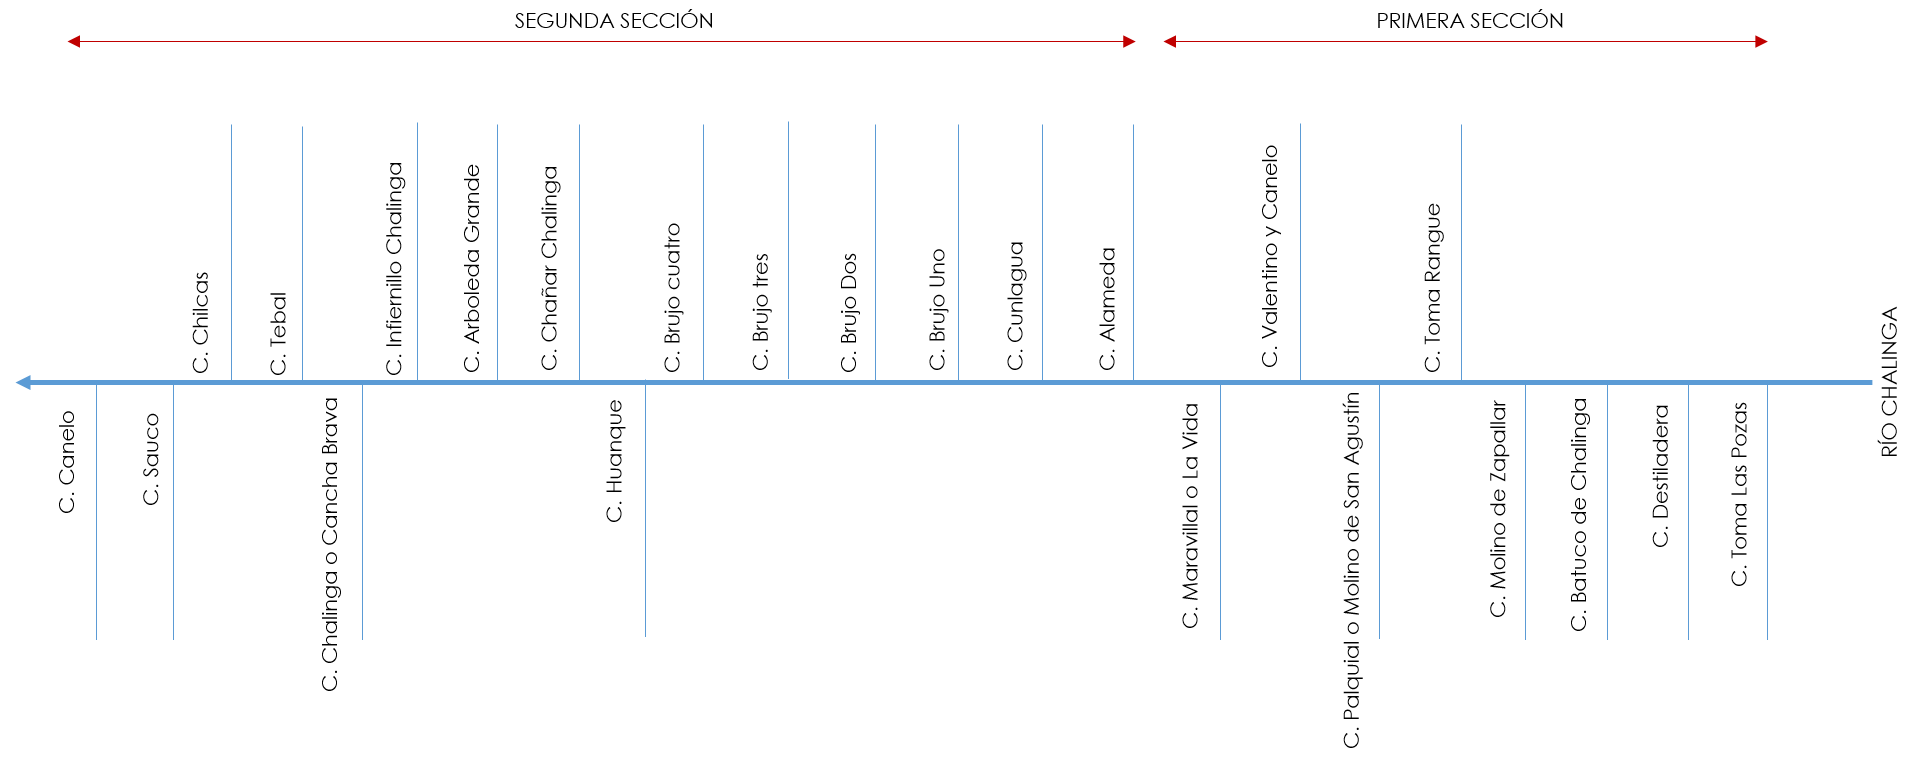
\includegraphics[width=\textwidth]{Logo/DiagramaChalinga}}
\caption{Diagrama Unifilar Junta de Vigilancia del Río Chalinga y sus Afluentes.}
\label{etiqueta_figura8}
\end{center}
\end{figure}

Se actualizaron los datos de acciones y capacidad de porteo a partir de la información levantada a la organización correspondiente (Junta de Vigilancia del Río Chalinga y sus Afluentes), de los canales:
\begin{itemize}

\item \textbf{Arboleda Grande}, con 98,76 acciones, equivalentes a 119 $l/s$.
\item \textbf{Chalinga o Cancha Brava}, con 104,93 acciones, equivalentes a 150 $l/s$.
\item \textbf{Huanque}, con 109,26 acciones, equivalentes a 140 $l/s$.\\

\end{itemize}

Se generó un escenario llamado \textit{Escenario Revestimiento}, el cual contiene la actualización del número de acciones asociada a los derechos nominales sobre el río Chalinga
y la pérdida por conducción equivalente a 0$\%$ \\
\\
Al correr tal escenario, el modelo muestra como el revestimiento de esta sección del río Chalinga, afecta de manera positiva la cobertura de la demanda agrícola, particularmente los cultivos anuales. Tal efecto muestra un 4$\%$ como promedio de mayor cobertura a lo largo de la serie temporal. Sin embargo, es en los momento de menor disponibilidad hídrica cuando los efectos son mayores, donde la cobertura aumenta en mas de un 10$\%$ en meses de mayor demanda.

\begin{figure}[H]
\begin{center}
\fbox{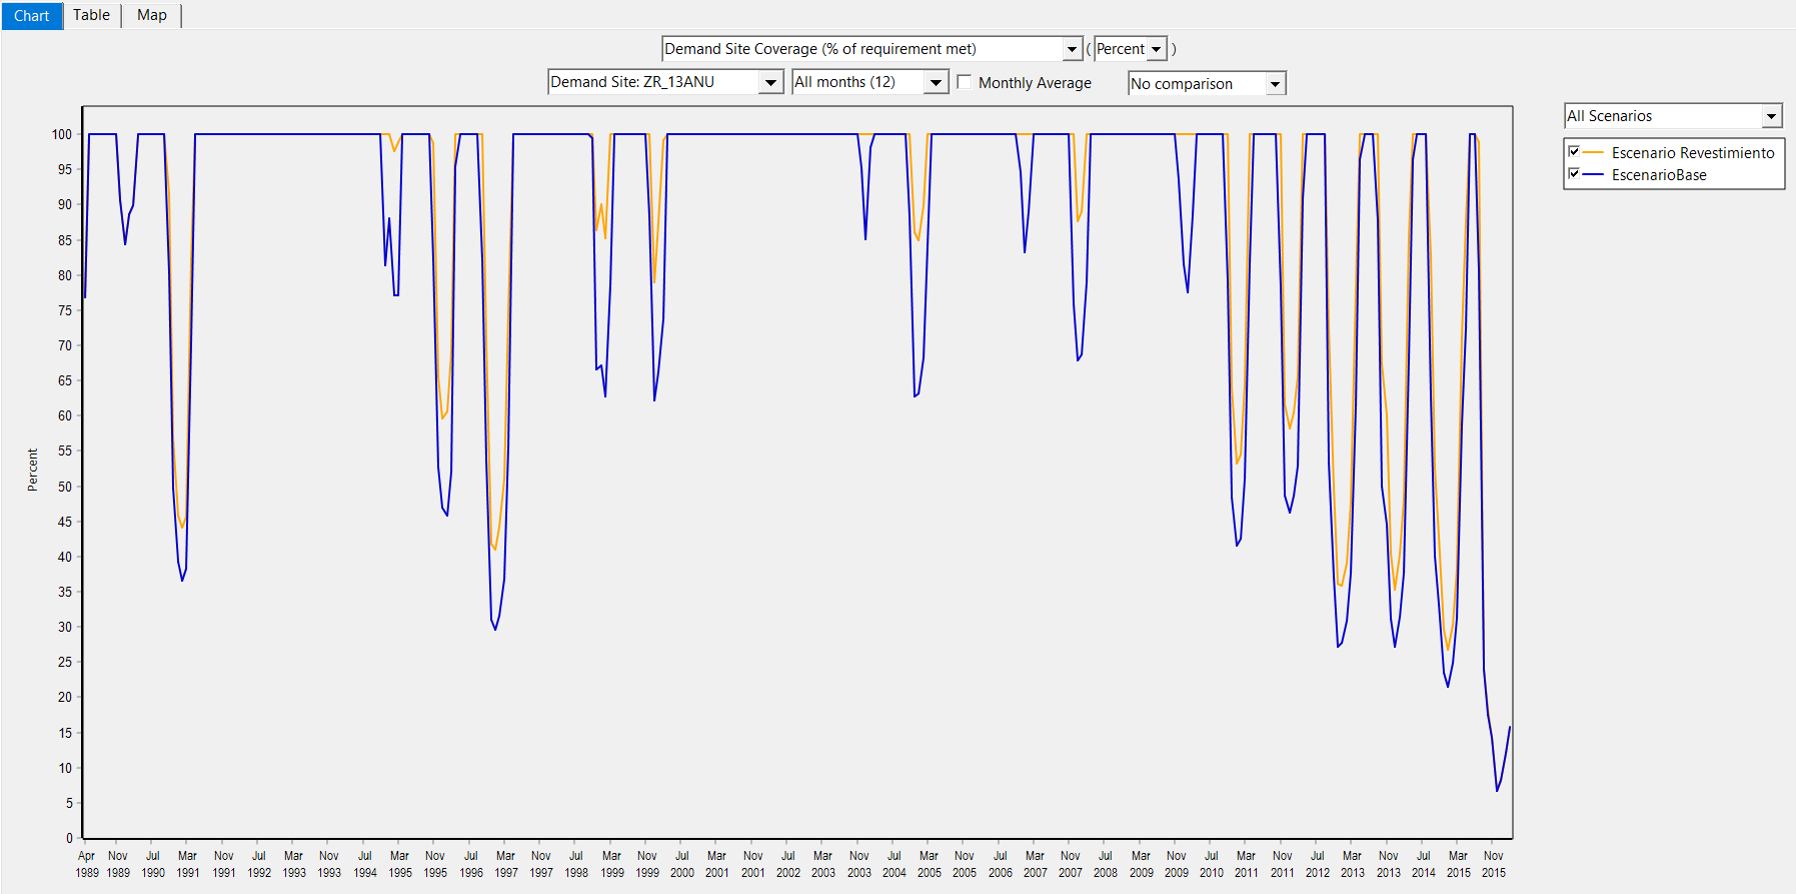
\includegraphics[width=\textwidth]{Logo/Validación1}}
\caption{Cobertura de la demanda de cultivos anuales ($\%$). Zona influenciada por los canales de la sección 2 del río Chalinga.}
\label{etiqueta_figura9}
\end{center}
\end{figure}

De igual manera la seguridad de la cobertura de la demanda de esta zona agrícola (cultivos anuales), sostuvo un aumento producto del revestimiento de sus canales a lo largo de la serie temporal. En el escenario base, la demanda fue satisfecha en un 100$\%$, el 68,5$\%$ de las oportunidades, mientras que en el escenario con revestimiento de canales, la seguridad aumentó a un 77,2\% (Figura \ref{etiqueta_figura10}).

\begin{figure}[H]
\begin{center}
\fbox{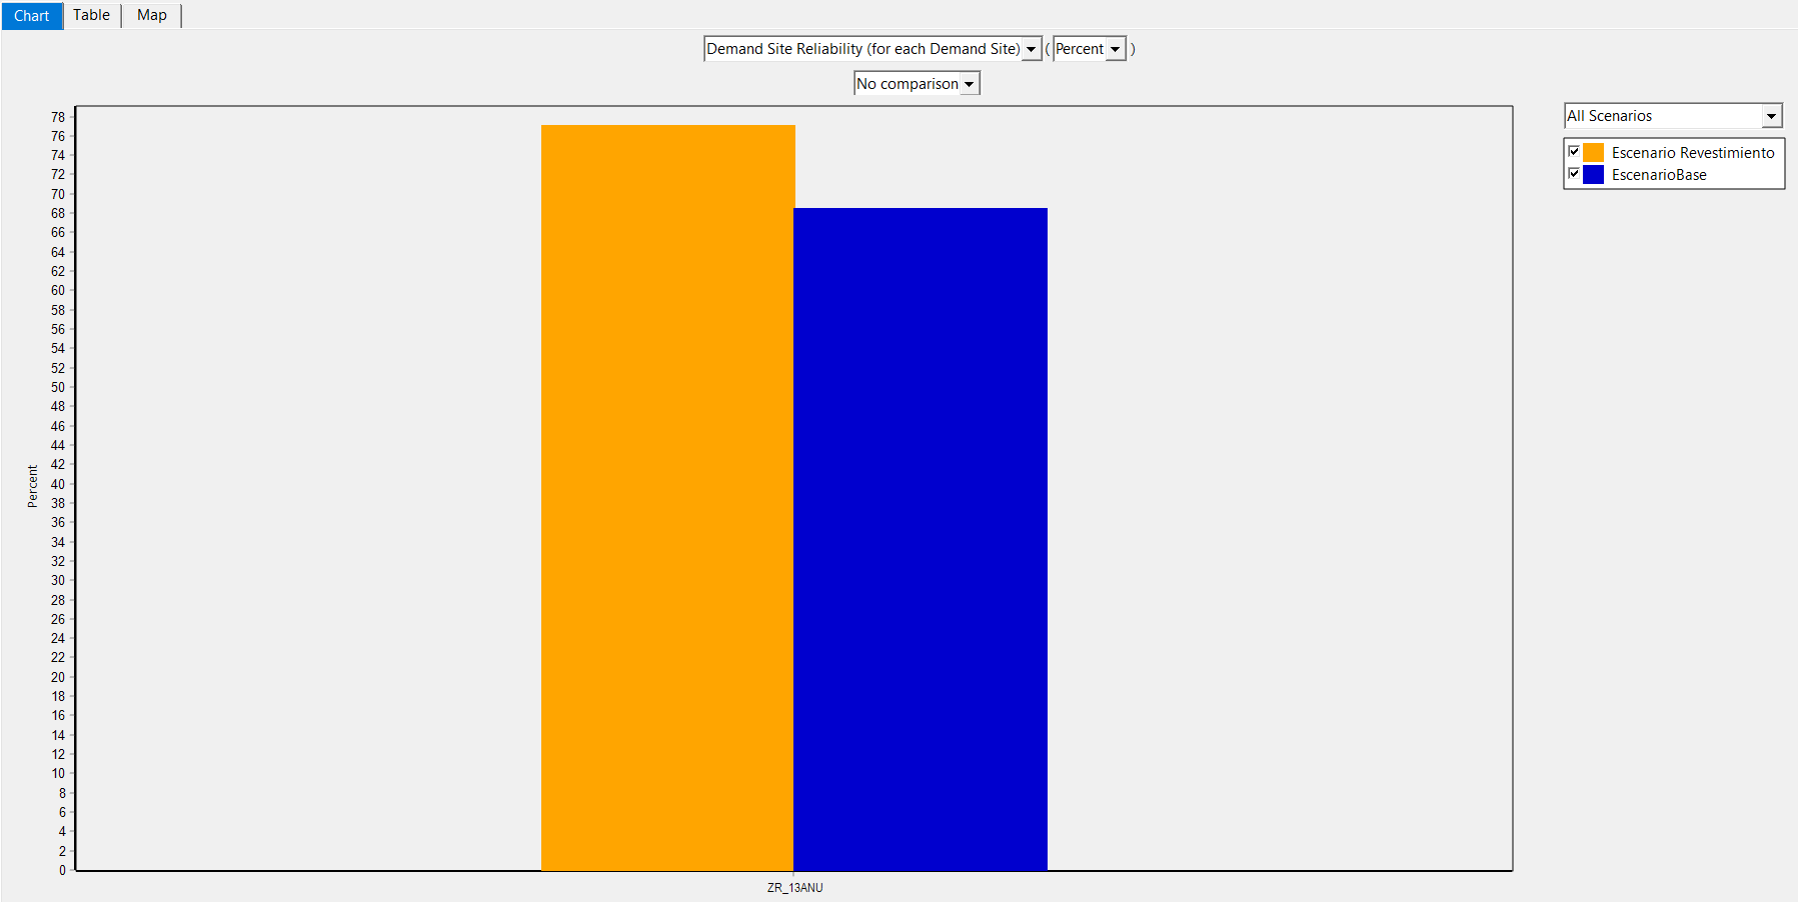
\includegraphics[width=\textwidth]{Logo/Validación2}}
\caption{Seguridad en la cobertura de la demanda de cultivos anuales ($\%$). Zona influenciada por los canales de la sección 2 del río Chalinga.}
\label{etiqueta_figura10}
\end{center}
\end{figure}

Los otros parámetros evaluados no tuvieron diferencias significativas entre ambos escenarios.


\subsubsection{Priorización de canales y tramos.}

La priorización de canales efectuada a los canales de validación, no consideró una clasificación en grupos de canales, ya que solo se dispone de 3 comunidades de aguas. Se realizó la matriz de las variables requeridas junto a las variables incorporadas de superficie (Cuadro \ref{tablav}). Posterior a esto se realizó un ordenamiento de las variables requeridas y variables de superficie, promediando los ordenamientos obtenemos el Plan de priorización (Cuadro \ref{tablaO}). La modelación hidrológica indica que los resultados de un mejoramiento en esta zona de la cuenca traería efectos positivos en la cobertura de la demanda agrícola y su seguridad. La priorización de tramos se realizará una vez que se obtenga todos los datos de la organización. 

\begin{landscape}
\begin{table} [H]
\centering
\caption{Variables requeridas por el Protocolo}
\label{tablav}
\begin{tabular}{|l|c|c|c|c|c|c|c|}
\hline
\textbf{Nombre Canal} & \textbf{N° Acciones} & \textbf{\begin{tabular}[c]{@{}c@{}}Capacidad de\\ porteo ($l/s$)\end{tabular}} & \textbf{\begin{tabular}[c]{@{}c@{}}N° de\\ Usuarios\end{tabular}} & \textbf{\begin{tabular}[c]{@{}c@{}}Superficie \\ bajo riego \\ ($ha$) \end{tabular}} & \textbf{\begin{tabular}[c]{@{}c@{}}Superficie \\ potencial\\ ($ha$) \end{tabular}} & \textbf{\begin{tabular}[c]{@{}c@{}}Volumen \\ recuperado \\ ($m^3/temporada$) \end{tabular}} & \textbf{\begin{tabular}[c]{@{}c@{}}Volumen recuperado \\ por $m^2$ a revestir\\ ($m^3/m^2 de revestido$) \end{tabular}} \\ \hline
Chalinga  		& 104,93 & 165 & 85 & 13,07 & 40 & 911075,0 & 167,4 \\ \hline
Arboleda Grande & 98,78 & 129,9 & 160 & 17,71 & 46,76 & 1368662,4 & 398,1 \\ \hline
Huanque			& 109,26 & 154 & 97 & 11,80 & 56,71 & 504576,0 & 157,0 \\ \hline
\end{tabular}
\end{table}

\begin{table} [H]
\centering
\caption{Ordenamiento por variables requeridas por el Protocolo}
\label{tablaO}
\begin{tabular}{|l|c|c|c|c|c|c|c|c|}
\hline
\textbf{Nombre Canal} & \textbf{N° Acciones} & \textbf{\begin{tabular}[c]{@{}c@{}}Capacidad de\\ porteo ($l/s$)\end{tabular}} & \textbf{\begin{tabular}[c]{@{}c@{}}N° de\\ Usuarios\end{tabular}} & \textbf{\begin{tabular}[c]{@{}c@{}}Superficie \\ bajo riego \\ ($ha$) \end{tabular}} & \textbf{\begin{tabular}[c]{@{}c@{}}Superficie \\ potencial\\ ($ha$) \end{tabular}} & \textbf{\begin{tabular}[c]{@{}c@{}}Volumen \\ recuperado \\ ($m^3/temporada$) \end{tabular}} & \textbf{\begin{tabular}[c]{@{}c@{}}Volumen recuperado \\ por $m^2$ a revestir\\ ($m^3/m^2 de revestido$) \end{tabular}} & \textbf{Priorización} \\ \hline
Chalinga  		& 2 & 1 & 3 & 2 & 3 & 2 & 2 & 2 \\ \hline
Arboleda Grande & 3 & 3 & 1 & 1 & 2 & 1 & 1 & 1 \\ \hline
Huanque			& 1 & 2 & 2 & 3 & 1 & 3 & 3 & 2 \\ \hline
\end{tabular}
\end{table}
\end{landscape}


\subsection{Resultados Actividades de Difusión}



\clearpage
\section{Impactos logrados a la fecha.}

\clearpage
\section{Problemas enfrentados.}

\clearpage
\section{Programa del próximo período.}

\clearpage
\section{Conclusiones y recomendaciones.}

\clearpage
\section{Anexos. Componente 2.}

\subsection{Diccionario S.I.G.}
\begin{longtable}{|p{3cm}|p{3.5cm}|p{3.5cm}|p{3.5cm}|}
	\caption{S.I.G. red hídrica, elementos de una Comunidad de aguas}\\
	
	\hline
	\textbf{S.I.G.} & \textbf{Componente} & \textbf{Atributo} & \textbf{Opción}\\
	\hline
	\endfirsthead
	
	\caption{S.I.G. red hídrica, elementos de una Comunidad de aguas \emph{(continuación)}}\\
	\hline
	\textbf{S.I.G.} & \textbf{Componente} & \textbf{Atributo} & \textbf{Opción}\\
	\hline
	\endhead
	
	\hline
	\endfoot
	
	\hline
	\endlastfoot    
	
	\multirow {45}{3cm}{Bocatoma} & \multirow {6}{3.5cm}{Barrera desviación} & \multirow {6}{3.5cm}{Tipo de Obra} &  Barrera Frontal\\	\cline{4-4}
	& & & Barrera Lateral\\	\cline{4-4}
	& & & Pata de Cabra\\	\cline{4-4}
    & & & Pretil Material Fluvial\\     \cline{4-4}
    & & & Otro\\     \cline{3-4}
    & & Dimensión & Ancho barrera\\    \cline{2-4}
    & \multirow {17}{3.5cm}{Canal de aducción} & \multirow {3}{3.5cm}{Tipo de Punto} &  Inicial\\    \cline{4-4}
    & & & Intermedio\\    \cline{4-4}
    & & & Final\\    \cline{3-4}
    & & \multirow {2}{3.5cm}{Tipo de Bocatoma} & Permanente\\    \cline{4-4}
    & & & Temporal\\    \cline{3-4}
    & & \multirow {3}{3.5cm}{Tipo de Fuente} & Gravitacional\\    \cline{4-4}
    & & & Bombeo\\    \cline{4-4}
    & & & Otro\\    \cline{3-4}
    & & \multirow {2}{3.5cm}{Ribera} & Izquierda\\    \cline{4-4}
    & & & Derecha\\    \cline{3-4}
    & & \multirow {5}{3.5cm}{Material} & Mezcla suelo\\    \cline{4-4}
    & & & Hormigón\\    \cline{4-4}
    & & & Madera\\    \cline{4-4}
    & & & Mampostería\\    \cline{4-4}
    & & & Otro\\    \cline{2-4}
    & \multirow {17}{3.5cm}{Compuerta de Carga} & \multirow {7}{3.5cm}{Fuente de Abastecimiento} &  Cauce Natural\\    \cline{4-4}
    & & & Canal\\    \cline{4-4}
    & & & Estero\\    \cline{4-4}
    & & & Quebrada Permanente\\    \cline{4-4}
    & & & Quebrada Eventual\\    \cline{4-4}
    & & & Vertiente\\    \cline{4-4}
    & & & Otro\\    \cline{3-4}
    & & \multirow {3}{3.5cm}{Material} & Metálica\\    \cline{4-4}
    & & & Madera\\    \cline{4-4}
    & & & Otro\\    \cline{3-4}
    & & \multirow {2}{3.5cm}{Sistema} & Con Mecanismo\\    \cline{4-4}
    & & & Manual\\    \cline{3-4}
    & & \multirow {4}{3.5cm}{Devolución} & No\\    \cline{4-4}
    & & & Compuerta\\    \cline{4-4}
    & & & Vertedero\\    \cline{4-4}
    & & & Compuerta y Vertedero\\    \cline{3-4}
    & & \multirow {3}{3.5cm}{Dimensiones Vertedero} & Ancho\\    \cline{4-4}
    & & & Alto Compuerta\\    \cline{4-4}
    & & & Ancho Compuerta\\    \cline{3-4} \pagebreak
    & & \multirow {5}{3.5cm}{Dimensiones Sección} & Largo\\    \cline{4-4} 
    & & & Alto Inicial\\    \cline{4-4}
    & & & Ancho Inicial\\    \cline{4-4}
    & & & Alto Final\\    \cline{4-4}
    & & & Ancho Final\\    \cline{2-4} 
    \multirow {17}{3cm}{Bocatoma} & \multirow {17}{3.5cm}{Sección de Control} & \multirow {11}{3.5cm}{Tipo} &  Escurrimiento crítico\\    \cline{4-4}
    & & & Regla limnimétrica\\    \cline{4-4}
    & & & Estación Limnigráfica\\    \cline{4-4}
    & & & Barrera con Reglilla\\    \cline{4-4}
    & & & Sección Rectangular con Regla\\    \cline{4-4}
    & & & Barrera Triangular\\    \cline{4-4}
    & & & Barrera Triangular y Regla\\    \cline{4-4}
    & & & Aforo de Garganta\\    \cline{4-4}
    & & & Aforo Parshall\\    \cline{4-4}
    & & & Sensor de Presión\\    \cline{4-4}
    & & & Otro\\    \cline{3-4}
    & & \multirow {3}{3.5cm}{Dimensiones Sección} & Ancho\\    \cline{4-4}
    & & & Largo\\    \cline{4-4}
    & & & Alto\\    \cline{3-4}
    & & \multirow {3}{3.5cm}{Dimensiones Parshall} & Convergencia\\    \cline{4-4}
    & & & Garganta\\    \cline{4-4}
    & & & Divergencia\\     \hline   
    \multirow {29}{3cm}{Conducción y distribución} & \multirow {29}{3.5cm}{Conducción} & \multirow {3}{3.5cm}{Tipo de Punto} &  Inicial\\	\cline{4-4}
	& & & Intermedio\\	\cline{4-4}
	& & & Final\\    \cline{3-4}
    & & \multirow {9}{3.5cm}{Forma} & Indefinida\\    \cline{4-4}
    & & & Rectangular\\    \cline{4-4}
    & & & Trapezoidal\\    \cline{4-4}
    & & & Túnel\\    \cline{4-4}
    & & & Circular\\    \cline{4-4}
    & & & Embovedado\\    \cline{4-4}
    & & & Parabólico\\    \cline{4-4}
    & & & Triangular\\    \cline{4-4}
    & & & Semi-circular\\    \cline{3-4}
	& & \multirow {4}{3.5cm}{Revestimiento} & Sin revestimiento\\    \cline{4-4}
    & & & 1/3 caras revestidas\\    \cline{4-4}
    & & & 2/3 caras revestidas\\    \cline{4-4}
    & & & 3/3 caras revestidas\\    \cline{3-4}  
    & & \multirow {13}{3.5cm}{Material} & Mezcla Suelo\\    \cline{4-4}
    & & & Hormigón\\    \cline{4-4}
    & & & Loseta\\    \cline{4-4}
    & & & Geomembrana\\    \cline{4-4}
    & & & Tubo HDPE\\    \cline{4-4}
    & & & Geomembrana asfáltica\\    \cline{4-4}
    & & & Hormigón Roca\\    \cline{4-4}
    & & & Mampostería\\    \cline{4-4}
    & & & Roca\\    \cline{4-4}
    & & & Lecho de río\\    \cline{4-4}
    & & & PVC\\    \cline{4-4}
    & & & Tubo metálico\\    \cline{4-4}
    & & & Otro\\    \cline{2-4} 
    \multirow {49}{3cm}{Conducción y distribución} & \multirow {30}{3.5cm}{Distribución} & \multirow {5}{3.5cm}{Función} &  Entrega\\	\cline{4-4}
	& & & Gestión Frontal\\    \cline{4-4}
    & & & Gestión Lateral\\    \cline{4-4}
    & & & Ramal\\    \cline{4-4}
    & & & Ramal\\    \cline{3-4}
	& & \multirow {9}{3.5cm}{Tipo} &  Compuerta Volante\\	\cline{4-4}
    & & & Compuerta Hoja\\    \cline{4-4}
    & & & Taco\\    \cline{4-4}
    & & & Captación Bomba\\    \cline{4-4}
    & & & Captación Gravitacional c/regulación\\    \cline{4-4}
    & & & Captación Gravitacional s/regulación\\    \cline{4-4}
    & & & Marco Partidor\\    \cline{4-4}
    & & & Solo Marco\\    \cline{4-4}
    & & & Otro\\    \cline{3-4}
    & & \multirow {11}{3.5cm}{Material} &  Metal\\	\cline{4-4}
    & & & Madera\\    \cline{4-4}
    & & & Tubo Metálico\\    \cline{4-4}
    & & & Tubo Plástico Rígido\\    \cline{4-4}
    & & & Manguera\\    \cline{4-4}
    & & & Suelo\\    \cline{4-4}
    & & & Piedra\\    \cline{4-4}
    & & & Lata\\    \cline{4-4}
    & & & Saco\\    \cline{4-4}
    & & & Hormigón\\    \cline{4-4}
    & & & Otro\\  \cline{2-4}
    & \multirow {25}{3.5cm}{Observaciones} & \multirow {25}{3.5cm}{Tipos} & Inicio Desborde\\ \cline{4-4}
    & & & Punto Desborde\\ \cline{4-4}
    & & & Fin Desborde\\ \cline{4-4}
    & & & Inicio Quebrada\\ \cline{4-4}
    & & & Punto Quebrada\\ \cline{4-4}
    & & & Fin Quebrada\\ \cline{4-4}
    & & & Inicio Derrumbe\\ \cline{4-4}
    & & & Punto Derrumbe\\ \cline{4-4}
    & & & Fin Derrumbe\\ \cline{4-4}
    & & & Cruce Camino Inicio\\ \cline{4-4}
    & & & Cruce Camino Fin\\ \cline{4-4}
    & & & Inicio Embancamiento\\ \cline{4-4}
    & & & Punto Embancamiento\\ \cline{4-4}
    & & & Fin Embancamiento\\ \cline{4-4}
    & & & Extracciones\\ \cline{4-4}
    & & & Inicio Contaminación\\ \cline{4-4}
    & & & Inicio Zona Poblada\\ \cline{4-4}
    & & & Fin Zona Poblada\\ \cline{4-4}
    & & & Zona de Filtración\\ \cline{4-4}
    & & & Aporte Continuo\\ \cline{4-4}
    & & & Aporte Eventual\\ \cline{4-4}
    & & & Cámara de Inspección\\ \cline{4-4}
    & & & Ramal Intermedio\\ \cline{4-4}
    & & & Ramal Fin\\ \cline{4-4}
    & & & Otro\\ \cline{2-4}
    \end{longtable}

\newpage
\subsection{Imágenes y listado de asistencia reunión Junta de Vigilancia Río Chalinga y sus afluentes.} \label{fotos_reunión}

Reunión con parte del Directorio y profesionales de la Junta de Vigilancia del Río Chalinga y sus afluentes.

\begin{figure}[H]
  \centering
\begin{subfigure}{.45\textwidth}
\hfill
  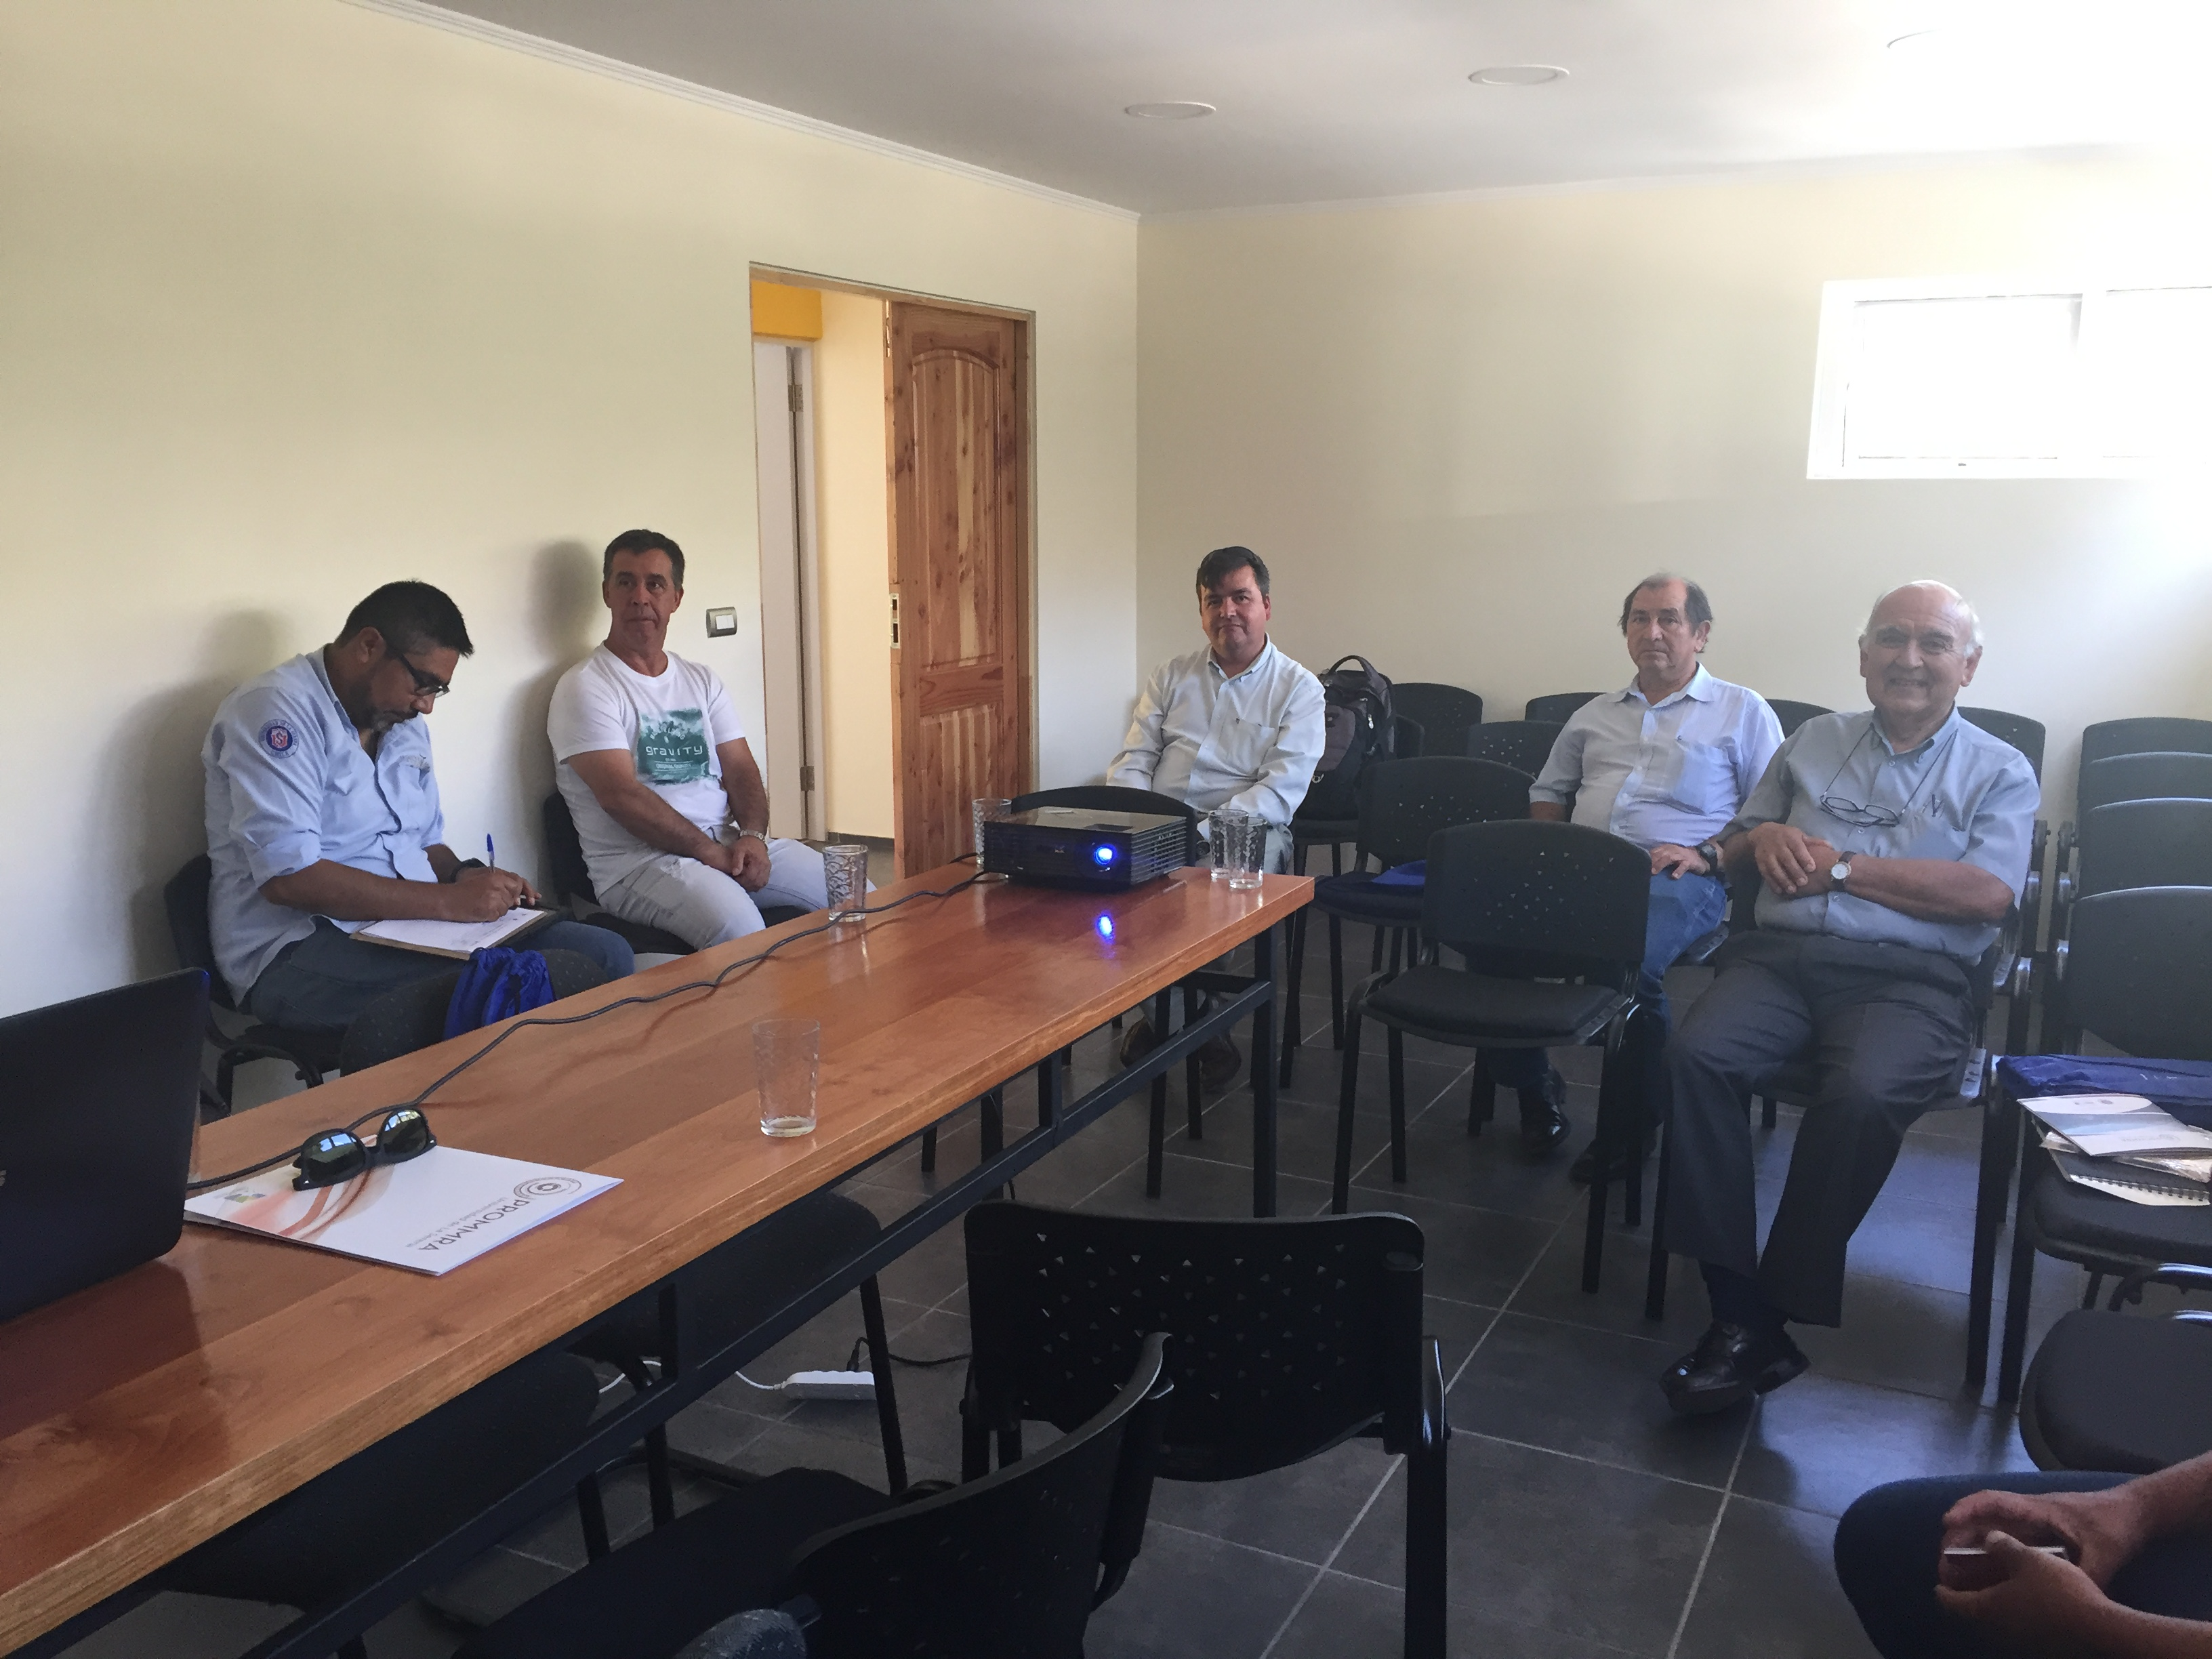
\includegraphics[width=\textwidth]{Reunión/Chalinga1.jpg}
\end{subfigure}
\hfill
\begin{subfigure}{.45\textwidth}
\hfill
  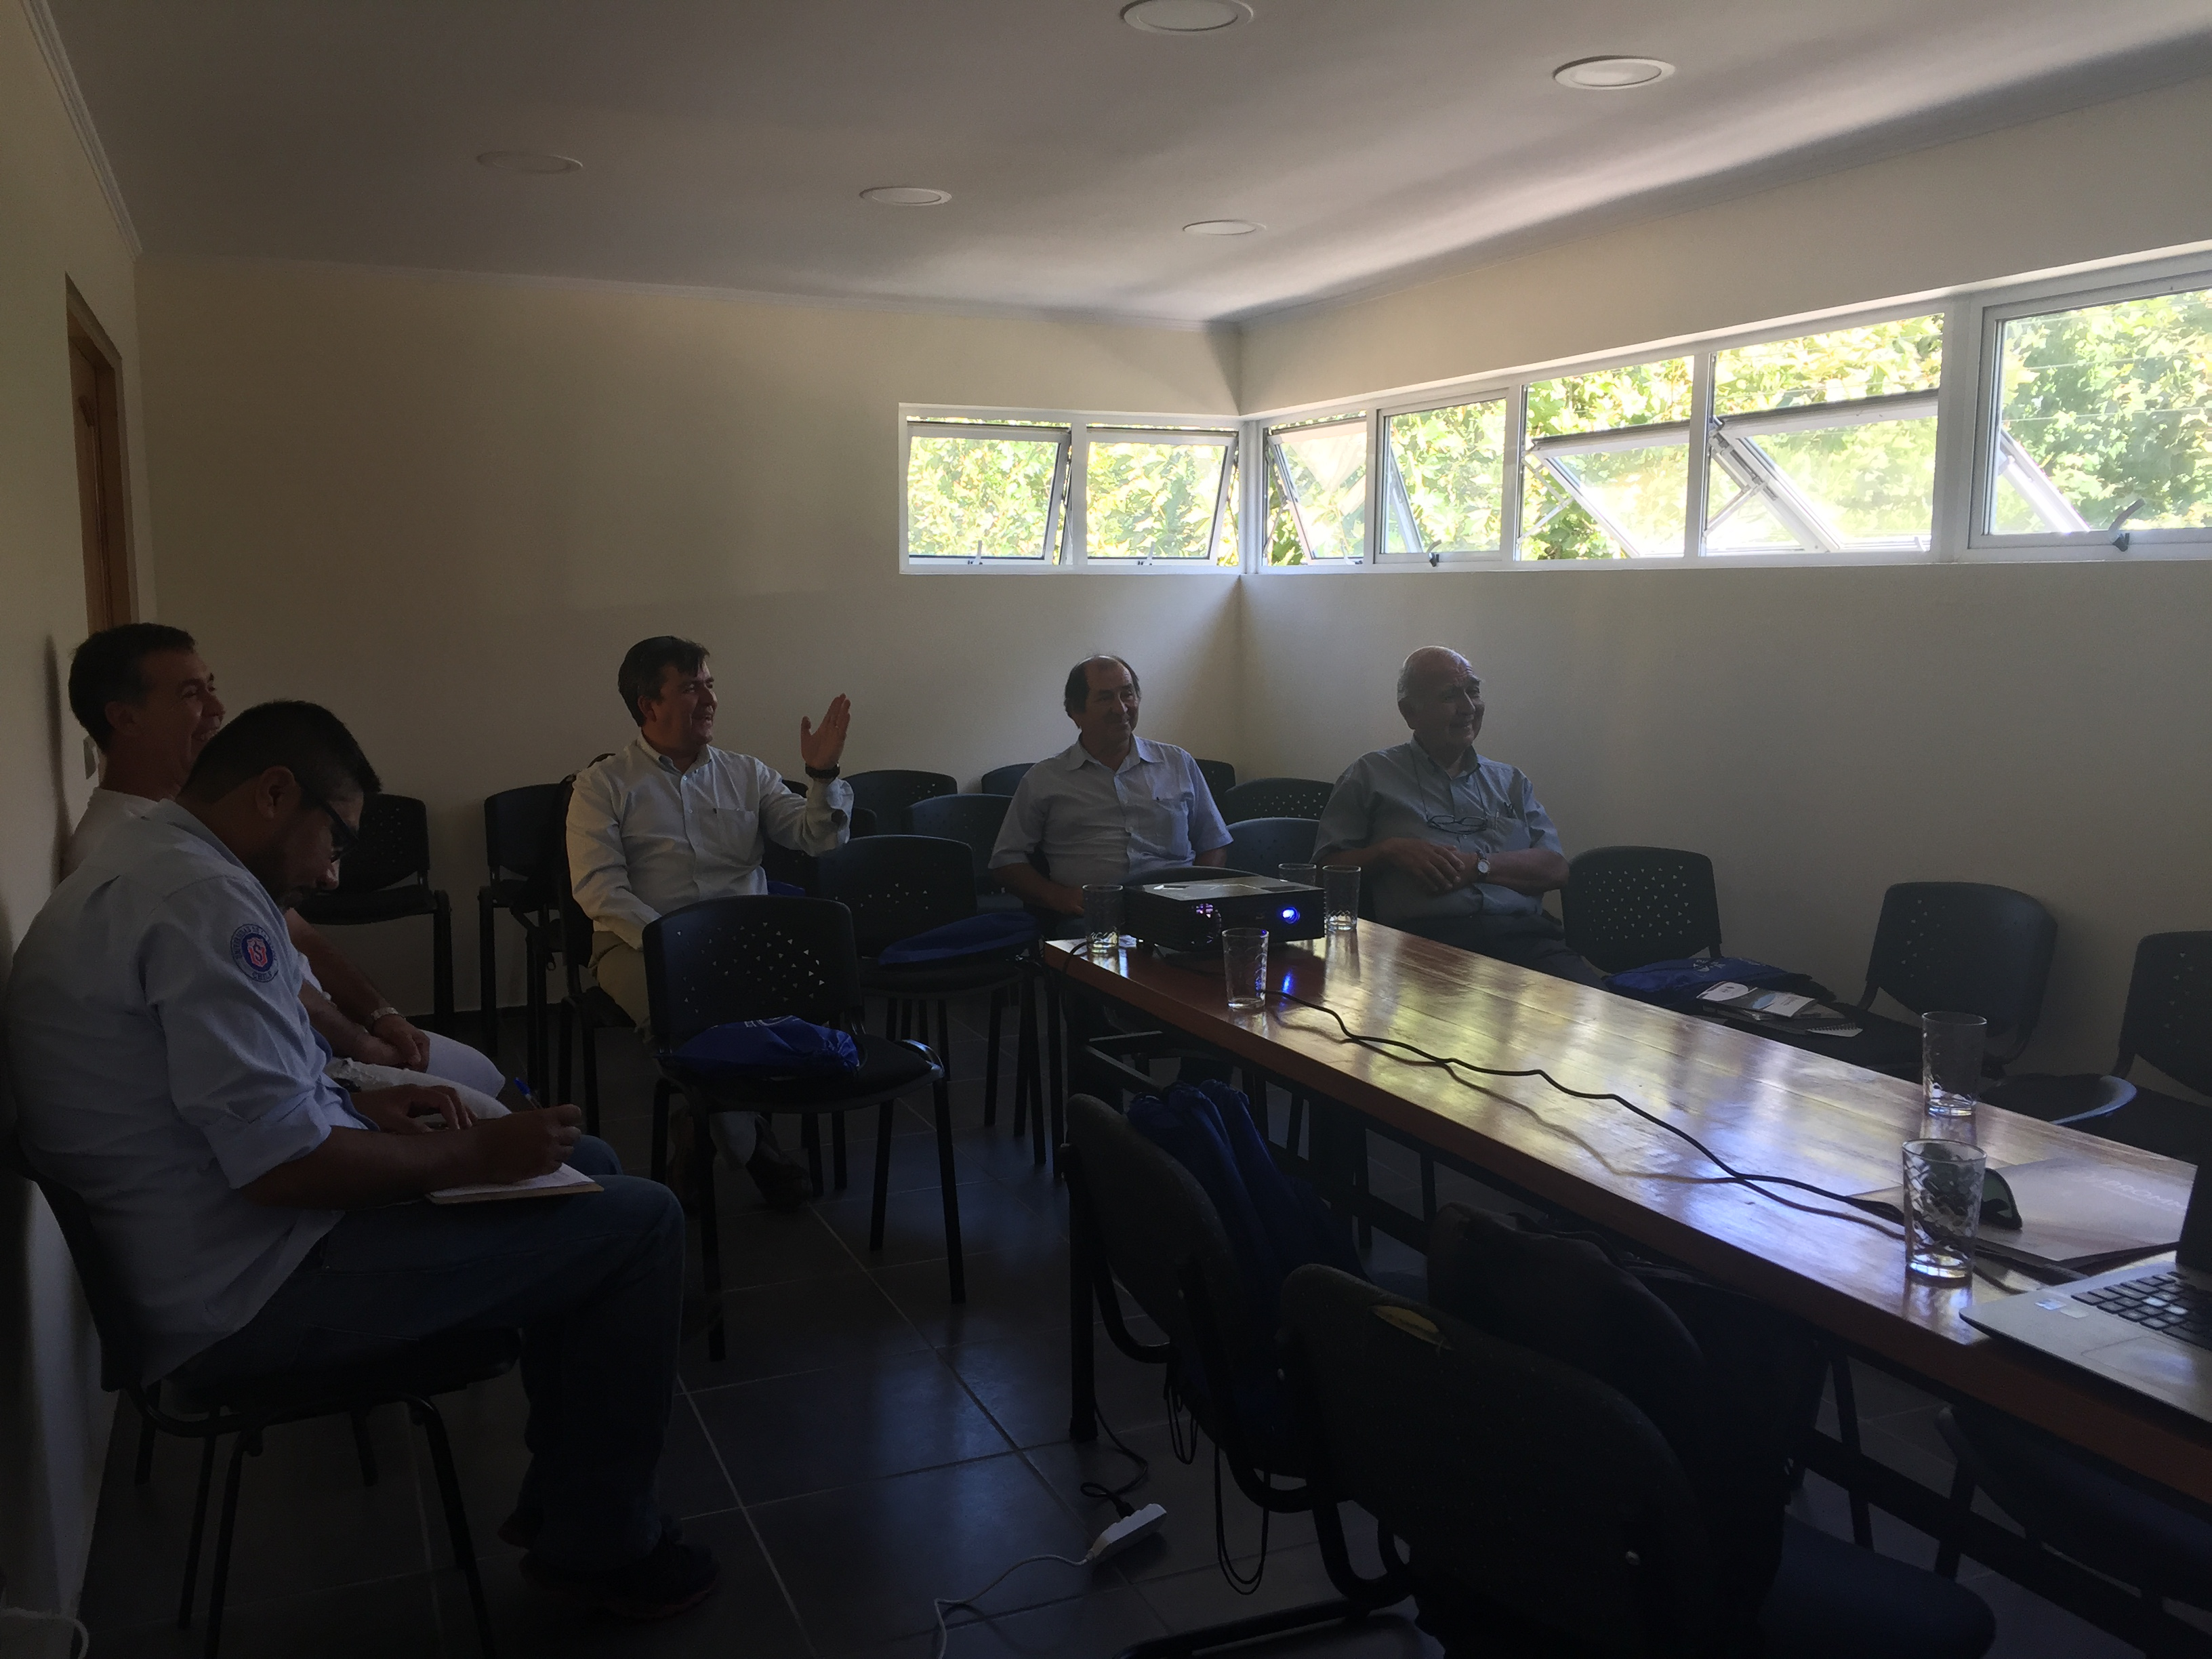
\includegraphics[width=\textwidth]{Reunión/Chalinga2.jpg} 
\end{subfigure}
\caption{Reunión Junta de Vigilancia del Río Chalinga y sus afluentes.}
\end{figure}

\begin{figure} [H]
	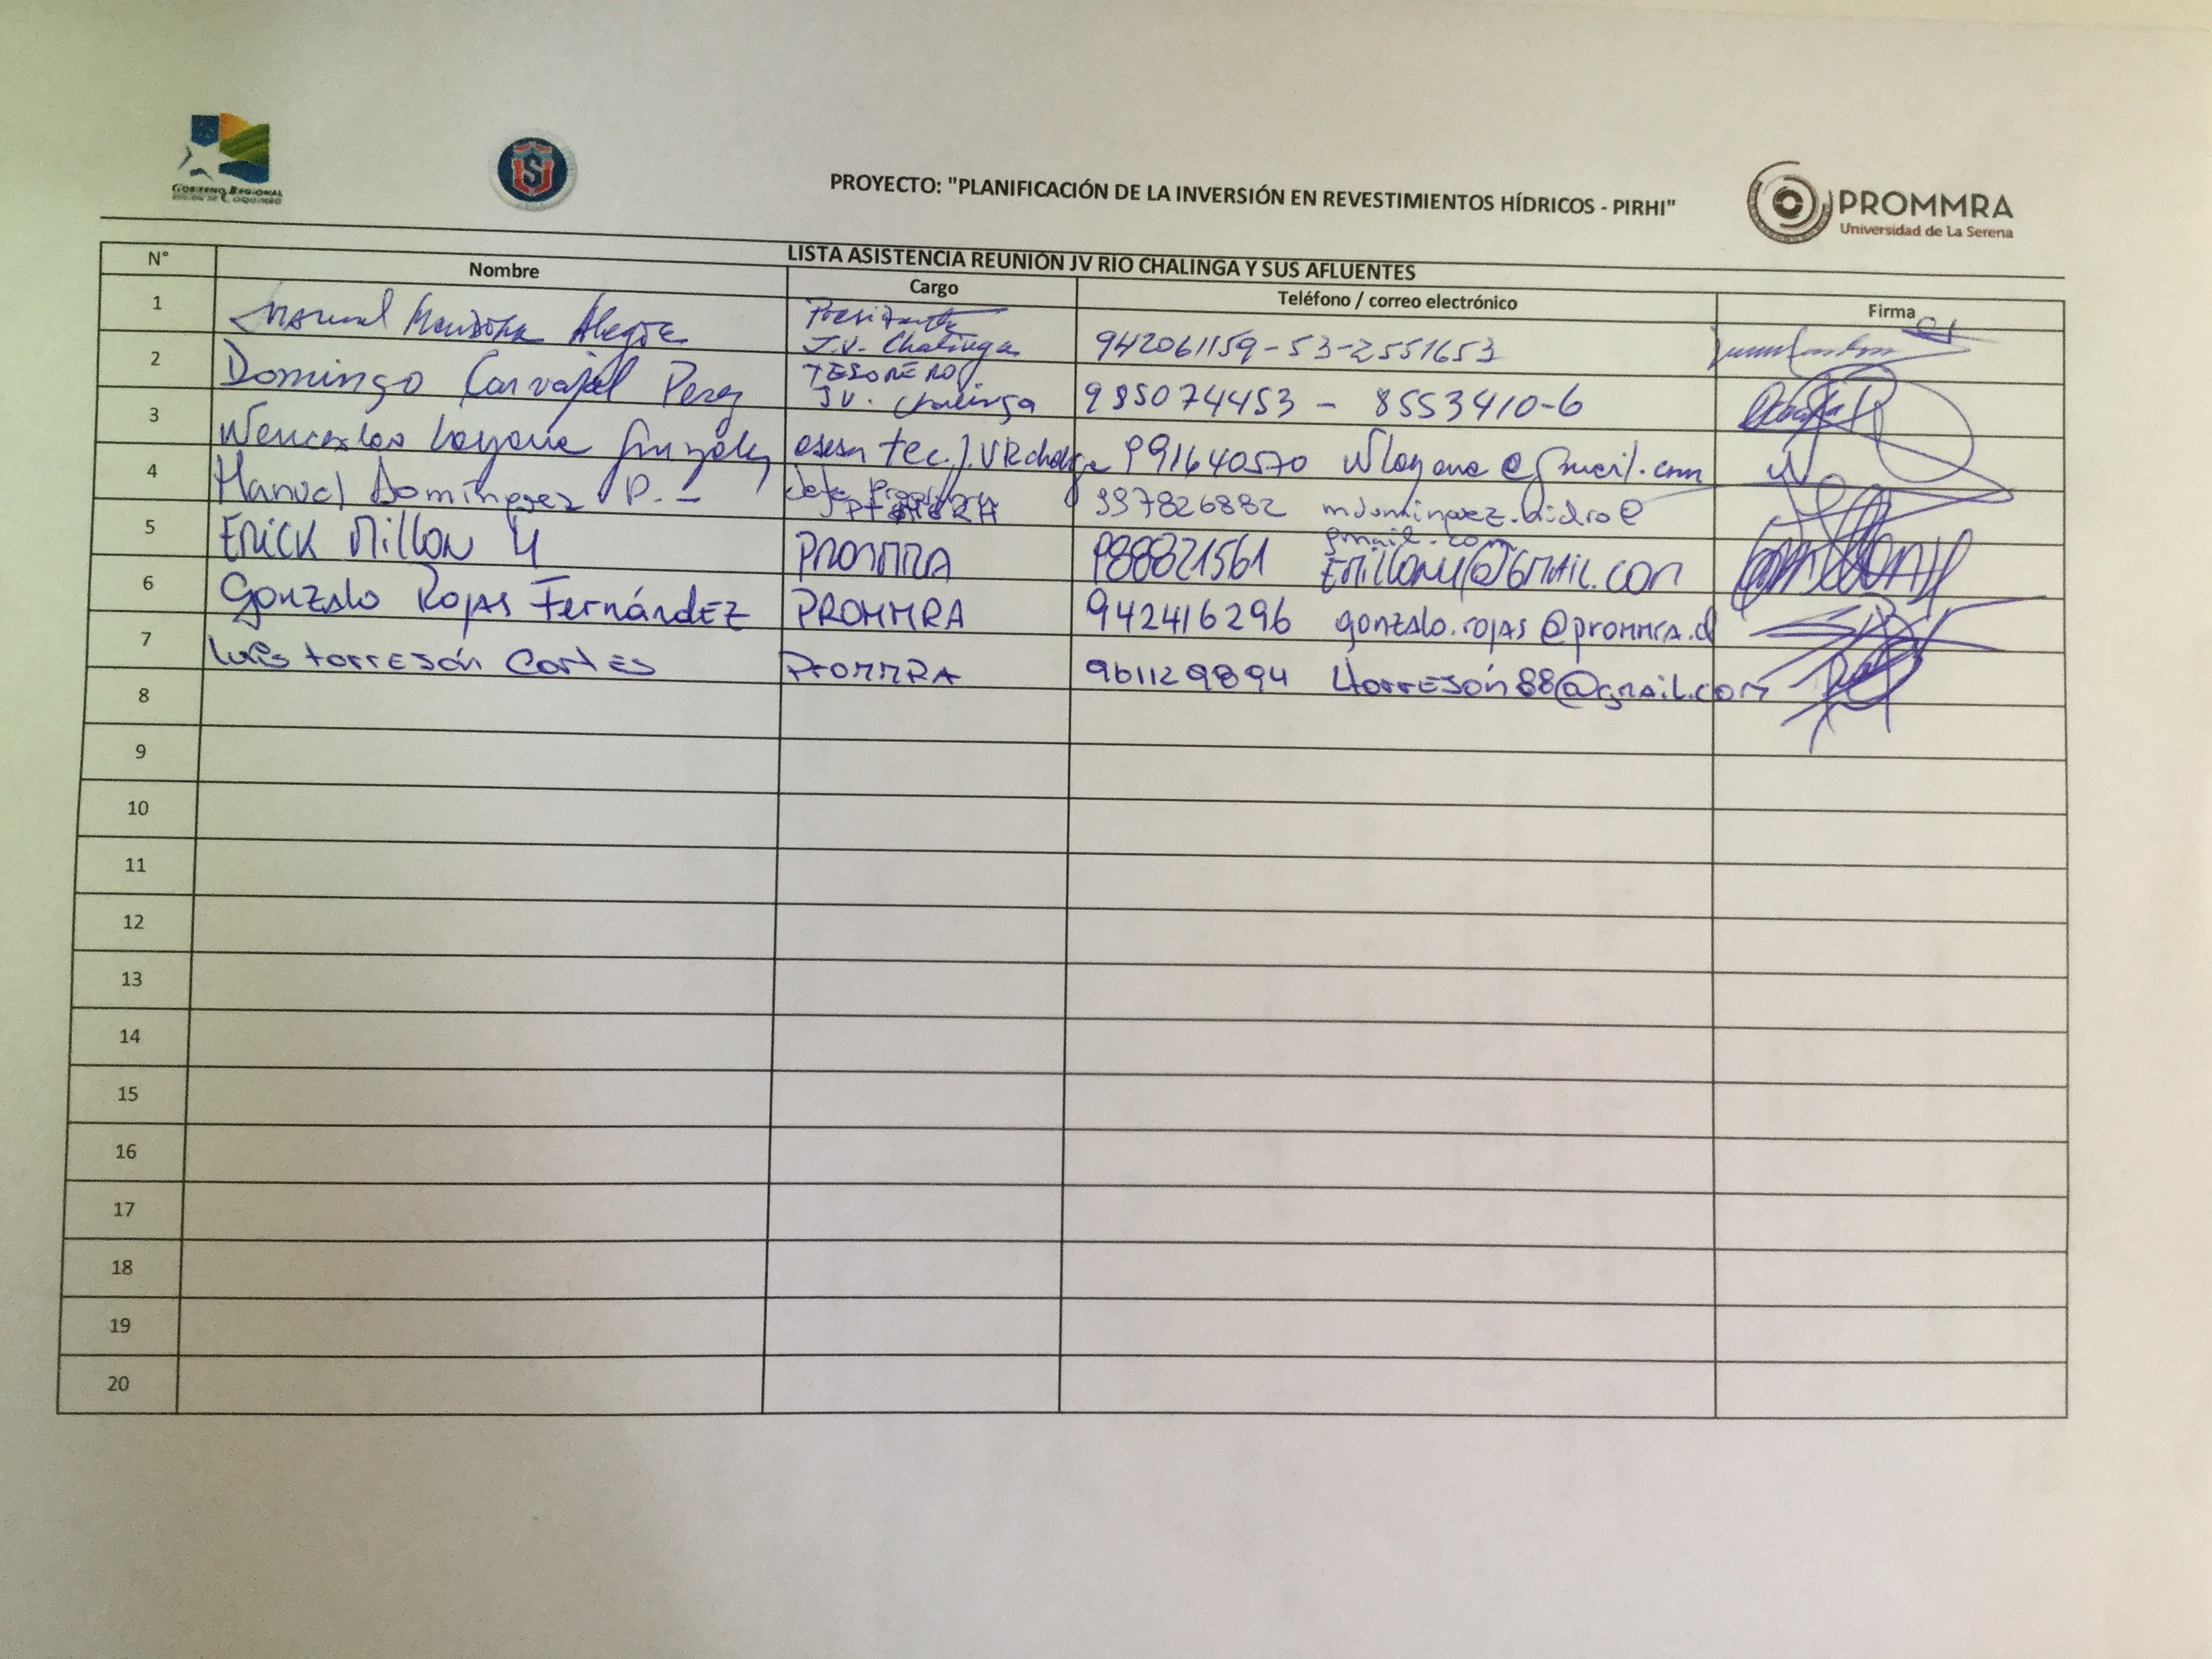
\includegraphics[width=\textwidth]{Reunión/Asistencia.jpg}
	\caption{Listado asistencia reunión Junta de Vigilancia Río Chalinga y sus afluentes.}
\end{figure}

\newpage

\subsection{Comunidades de aguas bajo jurisdicción de la Junta de Vigilancia Río Chalinga y sus afluentes.} \label{canales chalinga}

\begin{longtable}{|p{4cm}|p{3cm}|p{2cm}|p{2.5cm}|p{2cm}|}
	\caption{Comunidades de aguas Junta de Vigilancia Río Chalinga y sus afluentes.}\\
	
	\hline
	\textbf{Comunidad de aguas o canal} & \textbf{Fuente} & \textbf{Número de acciones} & \textbf{Litros/segundo} & \textbf{Número de usuarios}\\
	\hline
	\endfirsthead
	
	\caption{Comunidades de aguas Junta de Vigilancia Río Chalinga y sus afluentes \emph{(continuación)}}\\
	\hline
	\textbf{Comunidad de aguas o canal} & \textbf{Fuente} & \textbf{Número de acciones} & \textbf{Litros/segundo} & \textbf{Número de usuarios}\\
	\hline
	\endhead
	
	\hline
	\endfoot
	
	\hline
	\endlastfoot    
	
	Batuco de Chalinga 					& 1° sección río 	  	  	& 205,08 & 300 	 & 153	\\ \hline
	Molino de Zapallar 					& 1° sección río 	  	  	& 59 	 & 59 	 & 18 	\\ \hline
	Palquial o Molino de San Agustín	& 1° sección río 	  	  	& 245,2	 & 290 	 & 55 	\\ \hline
	Valentino o Canelo					& 1° sección río 	  	  	& 18,2 	 & 18,2	 & 2 	\\ \hline
	Maravillal o La Viña				& 1° sección río 	  	  	& 26,3	 & 31,56 & 9 	\\ \hline
	Alameda Derecha						& 1° sección río 	  	  	& 27,4	 & 28 	 & 15 	\\ \hline
	Gavino								& 1° sección río 	  	  	& 30	 & 30 	 & 43 	\\ \hline
	Piton								& 1° sección río 		  	& 10 	 & 10 	 & 43 	\\ \hline
	Destiladera							& 1° sección río 	  	  	& 100 	 & 76 	 & 43 	\\ \hline
	Ranque								& 1° sección río 	  	  	& 12 	 & 14 	 & 10 	\\ \hline
	Cunlagua							& 2° sección río 	  	  	& 116,1	 & 200 	 & 136 	\\ \hline
	Huanque								& 2° sección río 	  	  	& 109,26 & 140 	 & 97 	\\ \hline
	Chañar Chalinga						& 2° sección río 	  	  	& 40,26	 & 50	 & 26 	\\ \hline
	Arboleda Grande						& 2° sección río 	  	  	& 104,93 & 150 	 & 160 	\\ \hline
	El Tebal							& 2° sección río 	  	  	& 172 	 & 230	 & 259 	\\ \hline
	Chalinga o Cancha Brava				& 2° sección río 	 	  	& 98,78	 & 119	 & 85 	\\ \hline
	Chilcas								& 2° sección río 	  	  	& 74	 & 120 	 & 102 	\\ \hline
	Brujo Número Tres					& 2° sección río 	  	  	& S.I. 	 & S.I.	 & S.I.	\\ \hline
	Brujo Número Cuatro Infiernillo		& 2° sección río 	  	  	& S.I. 	 & S.I.	 & S.I.	\\ \hline
	Sauco								& 2° sección río 	  	  	& S.I. 	 & S.I.	 & S.I. \\ \hline
	Canelo								& 2° sección río 	  	  	& S.I. 	 & S.I.  & S.I.	\\ \hline
	Los Guindos							& 2° sección río 	 	  	& 224 	 & 28 	 & 28 	\\ \hline
	Quebrada Mala						& Quebrada Jarillas	 	  	& 272 	 & 16 	 & 13 	\\ \hline
	Quillayal							& Quebrada Jarillas	  	  	& 22 	 & 15 	 & 3 	\\ \hline
	Jarillas							& Quebrada Jarillas	  	  	& 445 	 & 69	 & 18 	\\ \hline
	Quillay Jarillas					& Quebrada Jarillas	  	  	& 12 	 & 8 	 & 2 	\\ \hline
	El Sauce							& Quebrada Jarillas	      	& 117 	 & 20 	 & 11 	\\ \hline
	Las Palmas							& Quebrada Jarillas	  	  	& 72 	 & 16 	 & 8 	\\ \hline
	Los Nogales							& Quebrada Jarillas	  	  	& 89 	 & 10 	 & 8 	\\ \hline
	Angostura							& Quebrada Jarillas	      	& 1,95 	 & 8 	 & 2 	\\ \hline
	La Verde							& Quebrada Cunlagua	 	  	& 190 	 & 63 	 & 36 	\\ \hline
	Las Barrancas						& Quebrada Cunlagua		  	& 192 	 & 26 	 & 24 	\\ \hline
	Zanjón								& Quebrada Cunlagua		  	& 94 	 & 16	 & 15 	\\ \hline
	Porfiado							& Quebrada Cunlagua		  	& 168 	 & 8 	 & 2 	\\ \hline
	El Carrizo							& Quebrada Manquehua	  	& 276 	 & 15 	 & 6 	\\ \hline
	Toma Lucillal (Lucillal 1)			& Quebrada Manquehua	  	& 101 	 & 9	 & 16 	\\ \hline
	Lucillay (Lucillal 2)				& Quebrada Manquehua 	  	& 65	 & 7 	 & 10 	\\ \hline
	Tomas Las Mellizas Número Uno		& Quebrada Manquehua  	  	& 91,75  & 17 	 & 19 	\\ \hline
	Las Mellizas Número Dos				& Quebrada Manquehua      	& 81	 & 8 	 & 10 	\\ \hline
	Quillayal							& Quebrada Manquehua 	  	& 192 	 & 12 	 & 6 	\\ \hline
	Toma El Canelo						& Quebrada Manquehua 	  	& 96 	 & 12 	 & 5 	\\ \hline
	Toma Las Barrancas					& Quebrada Manquehua 	  	& 84 	 & 12 	 & 4 	\\ \hline
	Toma El Algarrobo					& Quebrada Manquehua  	  	& 168 	 & 15 	 & 14 	\\ \hline
	Peñon								& Quebrada Manquehua  	  	& 192 	 & 23 	 & 8 	\\ \hline
	EL Piche							& Quebrada El Piche  	  	& 216 	 & 20 	 & 4 	\\ \hline
	Vertiente San Francisco				& Vertiente San Francisco 	& 4 	 & 8 	 & 4 	\\ \hline
	Toma San Francisco					& Vertiente Toma San Francisco 	& 146 	 & 8 	& 14 	\\ \hline
	Vertiente Los Manantiales			& Vertiente Los Manantiales & 1,5 	 & 15 	 & 3 	\\ \hline
	Vertiente El Arroyo					& Vertiente Los Manantiales & 168 	 & 8 	 & 3 	\\ \hline
	Vertientes Los Paltos				& Vertiente Los Paltos		& 168 	 & 2 	 & 8 	\\ \hline
	Vertientes Las Casas				& Vertiente Las Casas		& 5,9 	 & 7 	 & 7 	\\ \hline
	Vertiente Canelo					& Vertiente Canelo			& 96 	 & 12 	 & 20 	\\ \hline
    \end{longtable}

\newpage
\subsection{Entrevista representante Junta de Vigilancia Río Chalinga y sus afluentes.} \label{Entrevista OUA's}

\begin{figure} [H]
  \fbox{\includegraphics[height=19cm]{Entrevistas OUA's y CA's/Arboleda_grande.pdf}}
	\caption{Entrevista Comunidad de aguas Arboleda grande.}
\end{figure}
\clearpage

\subsection{Entrevistas representantes Comunidades de Aguas de la Junta de Vigilancia Río Chalinga y sus afluentes.} \label{Entrevista CA's}

\begin{figure} [H]
  \fbox{\includegraphics[height=19cm]{Entrevistas OUA's y CA's/Arboleda_grande.pdf}}
	\caption{Entrevista Comunidad de aguas Arboleda grande.}
\end{figure}
\clearpage

\textbf{- Comunidad de Aguas Chalinga o Cancha Brava.}

\begin{figure}[H]
  \centering
\begin{subfigure}{.45\textwidth}
\hfill
  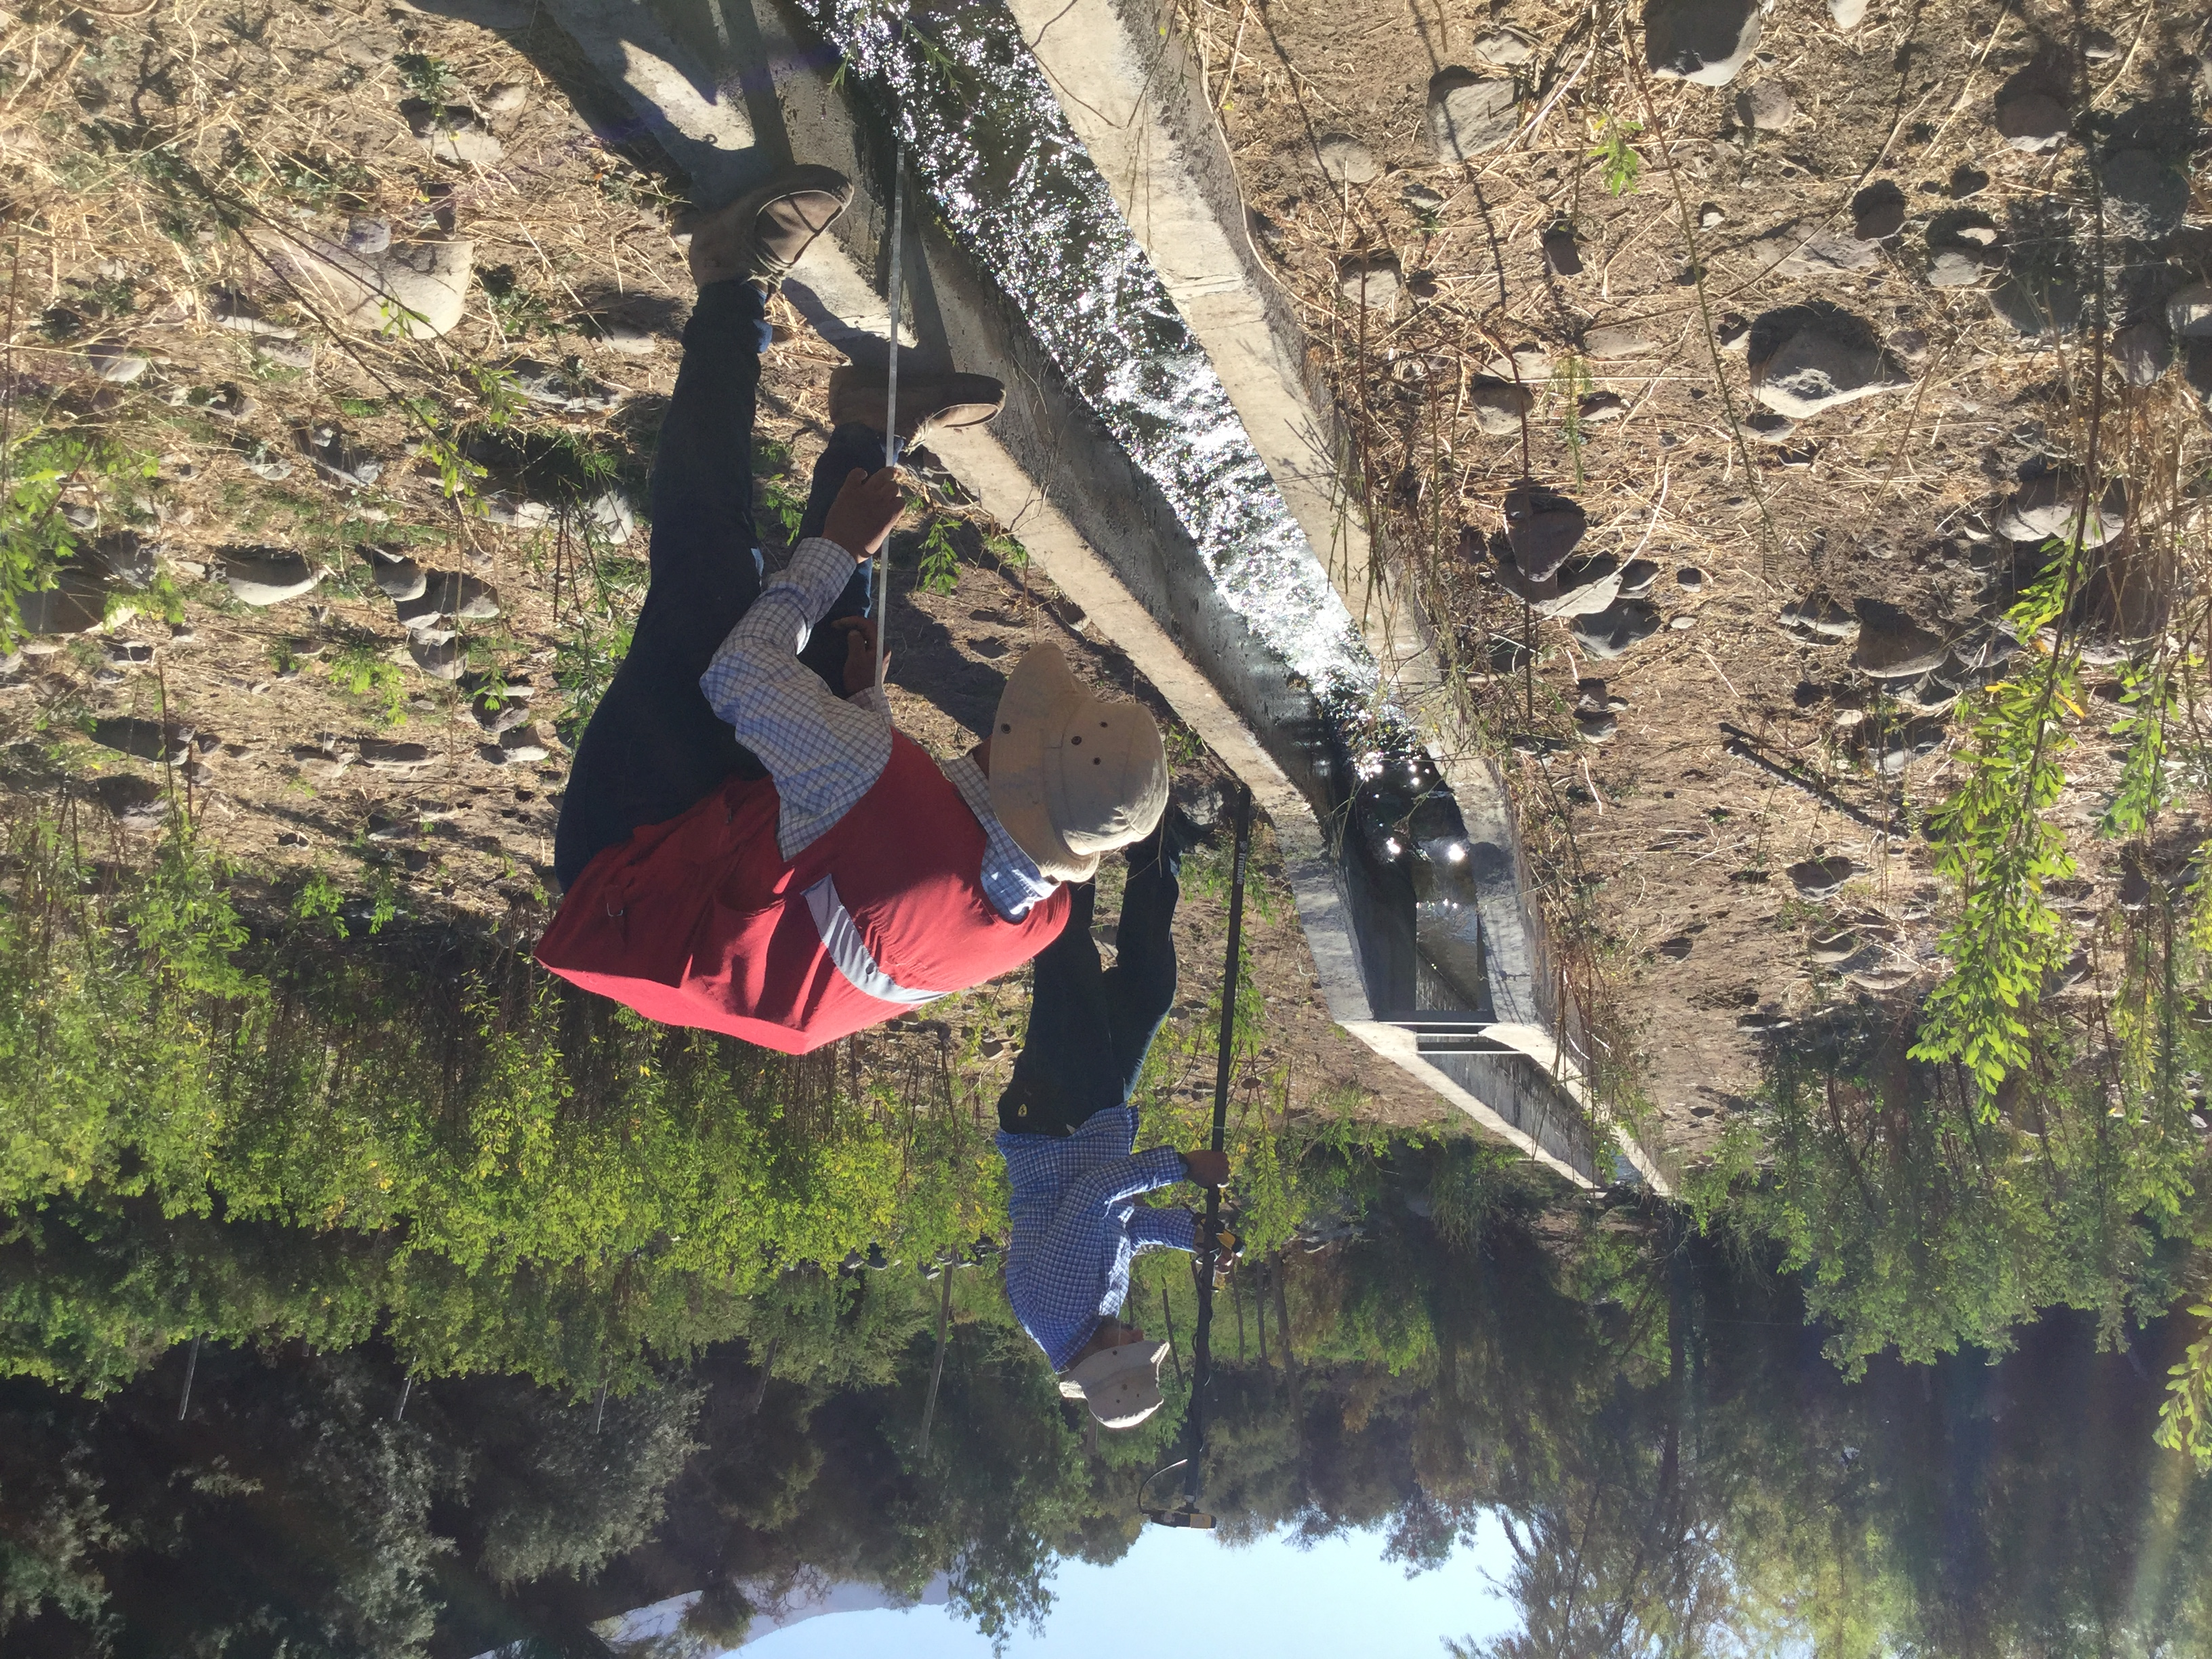
\includegraphics[angle= 180, width=\textwidth]{Foto/ch1.jpg}
\end{subfigure}
\hfill
\begin{subfigure}{.45\textwidth}
\hfill
  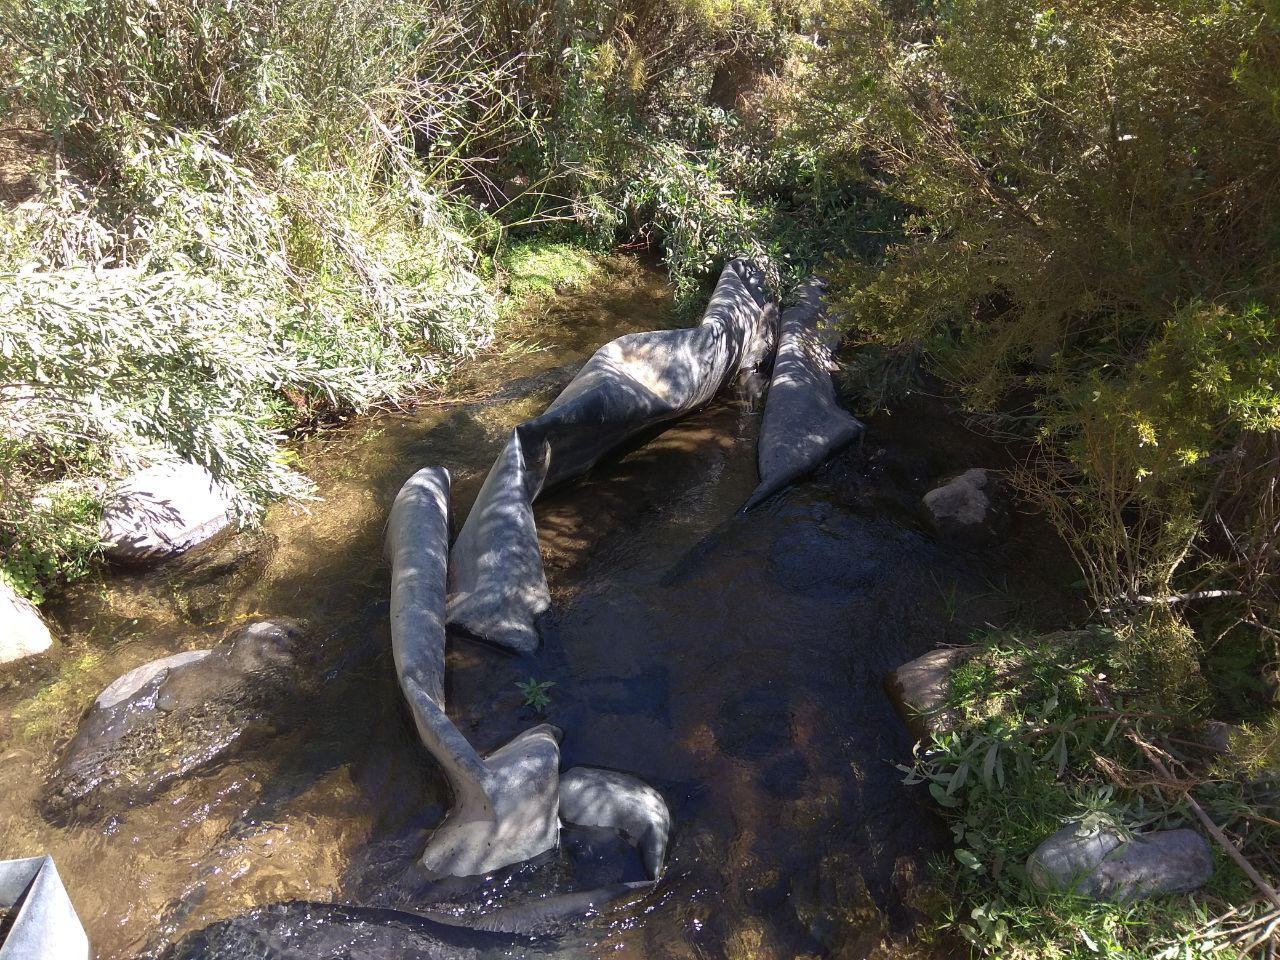
\includegraphics[width=\textwidth]{Foto/ch2.jpg} 
\end{subfigure}
\caption{Caracterización de infraestructura hídrica para el S.I.G. de Canal Chalinga o Cancha Brava, cuenca del río Chalinga.}
\end{figure}

\begin{figure}[H]
  \centering
\begin{subfigure}{.45\textwidth}
\hfill
  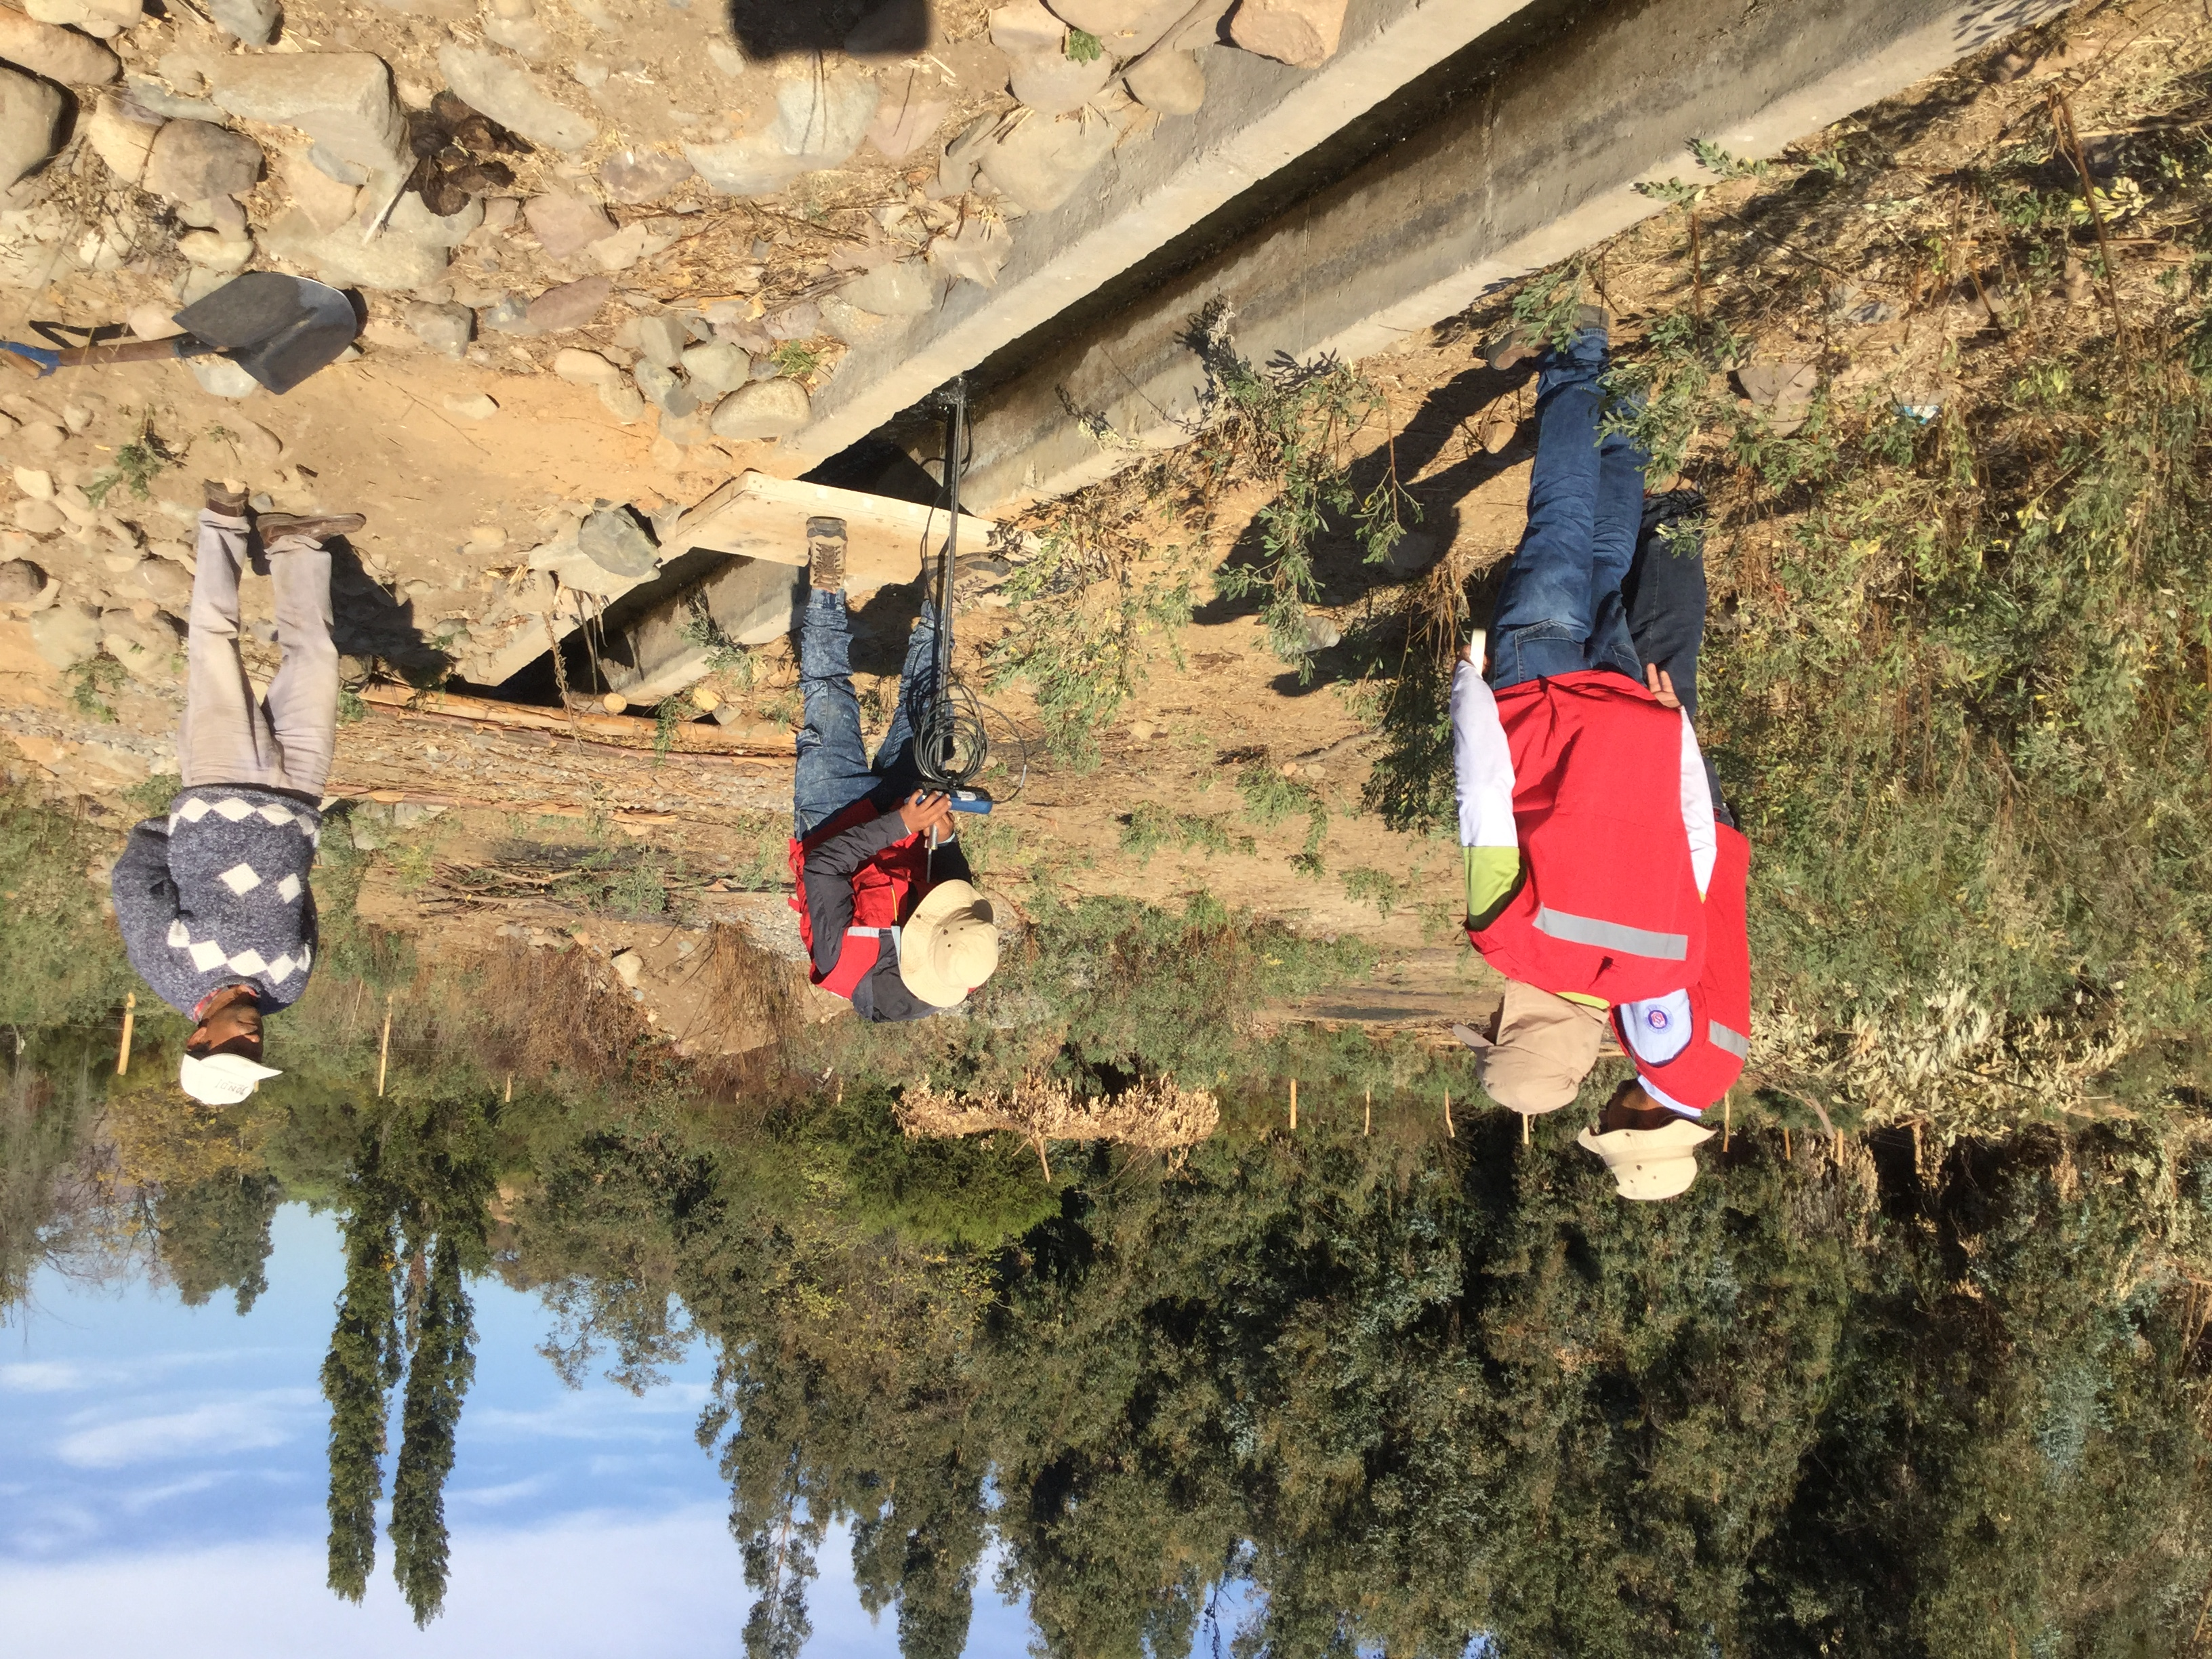
\includegraphics[angle= 180, width=\textwidth]{Foto/ch3.jpg}
\end{subfigure}
\hfill
\begin{subfigure}{.45\textwidth}
\hfill
  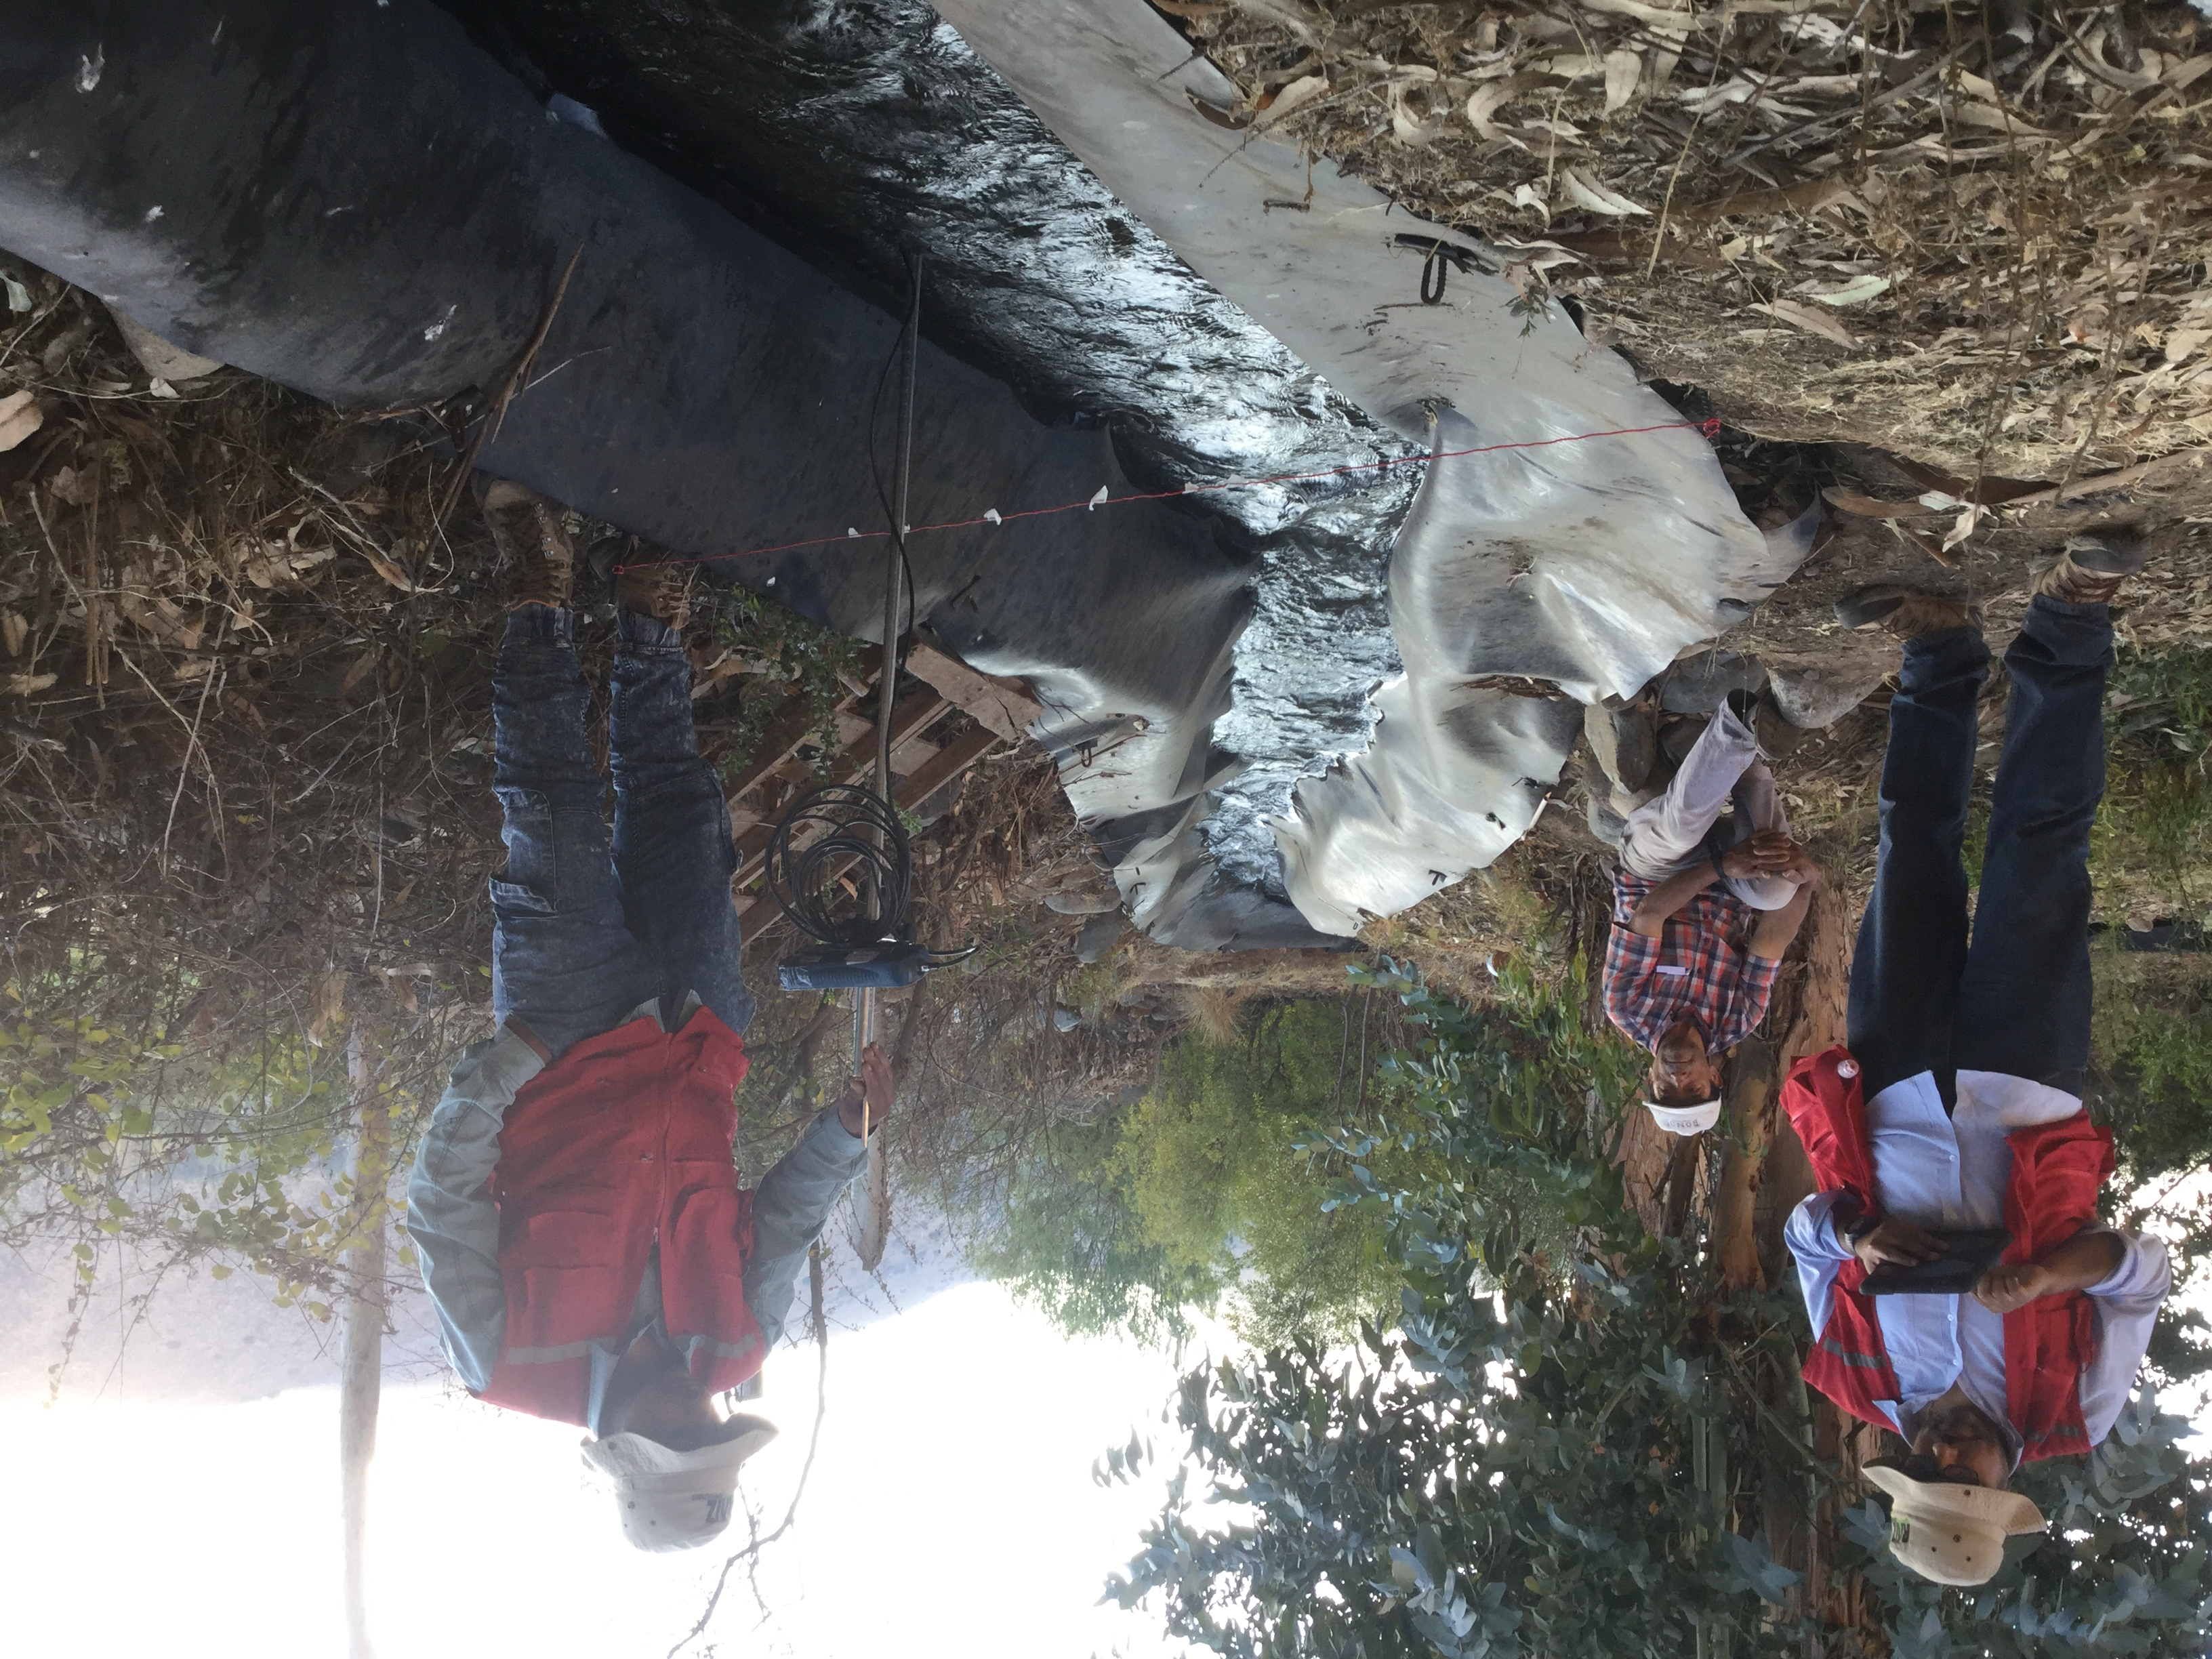
\includegraphics[angle= 180, width=\textwidth]{Foto/ch4.jpg} 
\end{subfigure}
\caption{Aforos de caudal Canal Chalinga o Cancha Brava, cuenca río Chalinga.}
\end{figure}
\clearpage

\textbf{- Comunidad de Aguas Arboleda Grande.}

\begin{figure}[H]
  \centering
\begin{subfigure}{.45\textwidth}
\hfill
  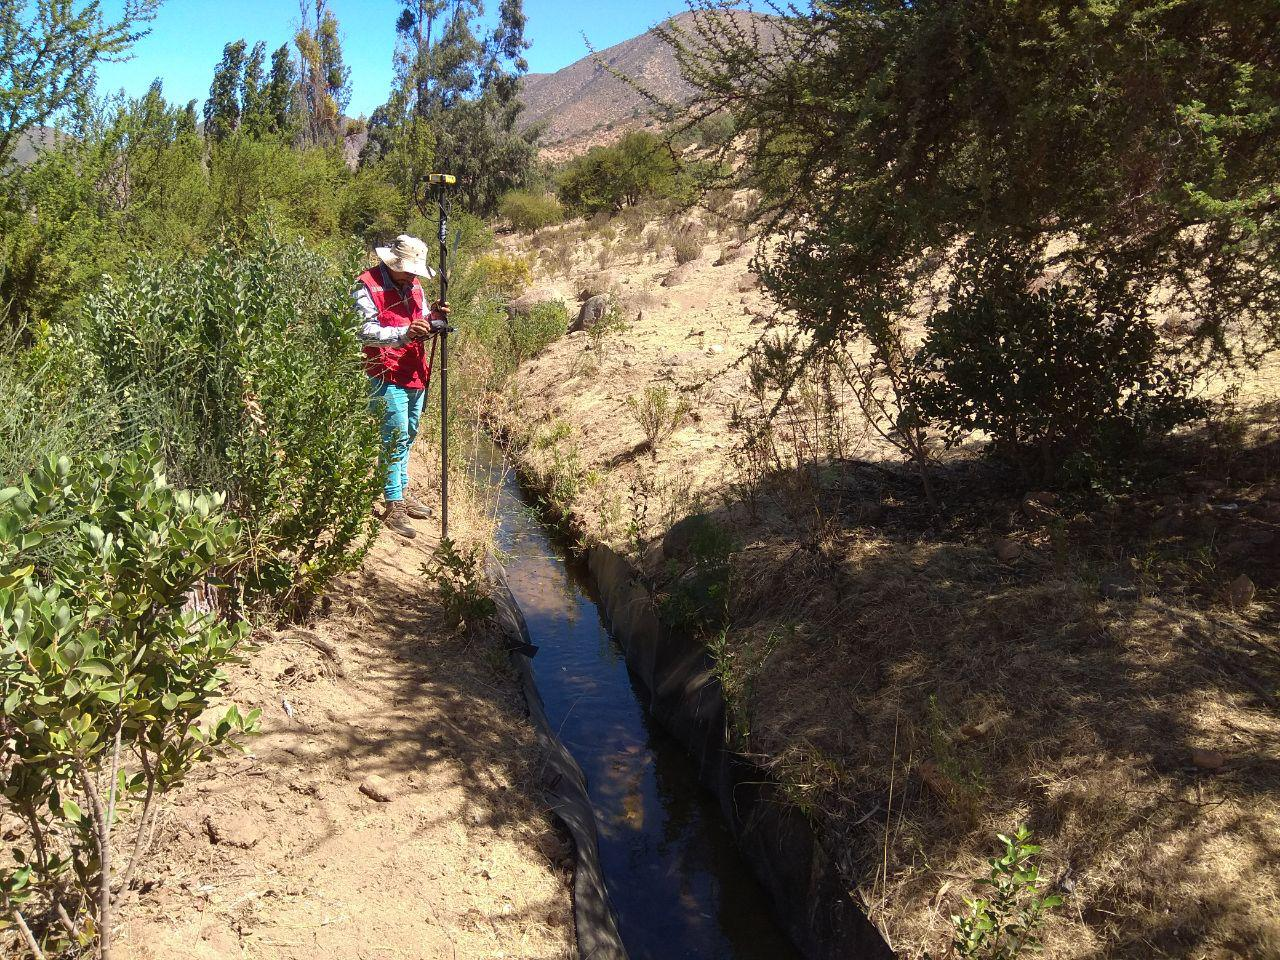
\includegraphics[width=\textwidth]{Foto/a1.jpg}
\end{subfigure}
\hfill
\begin{subfigure}{.45\textwidth}
\hfill
  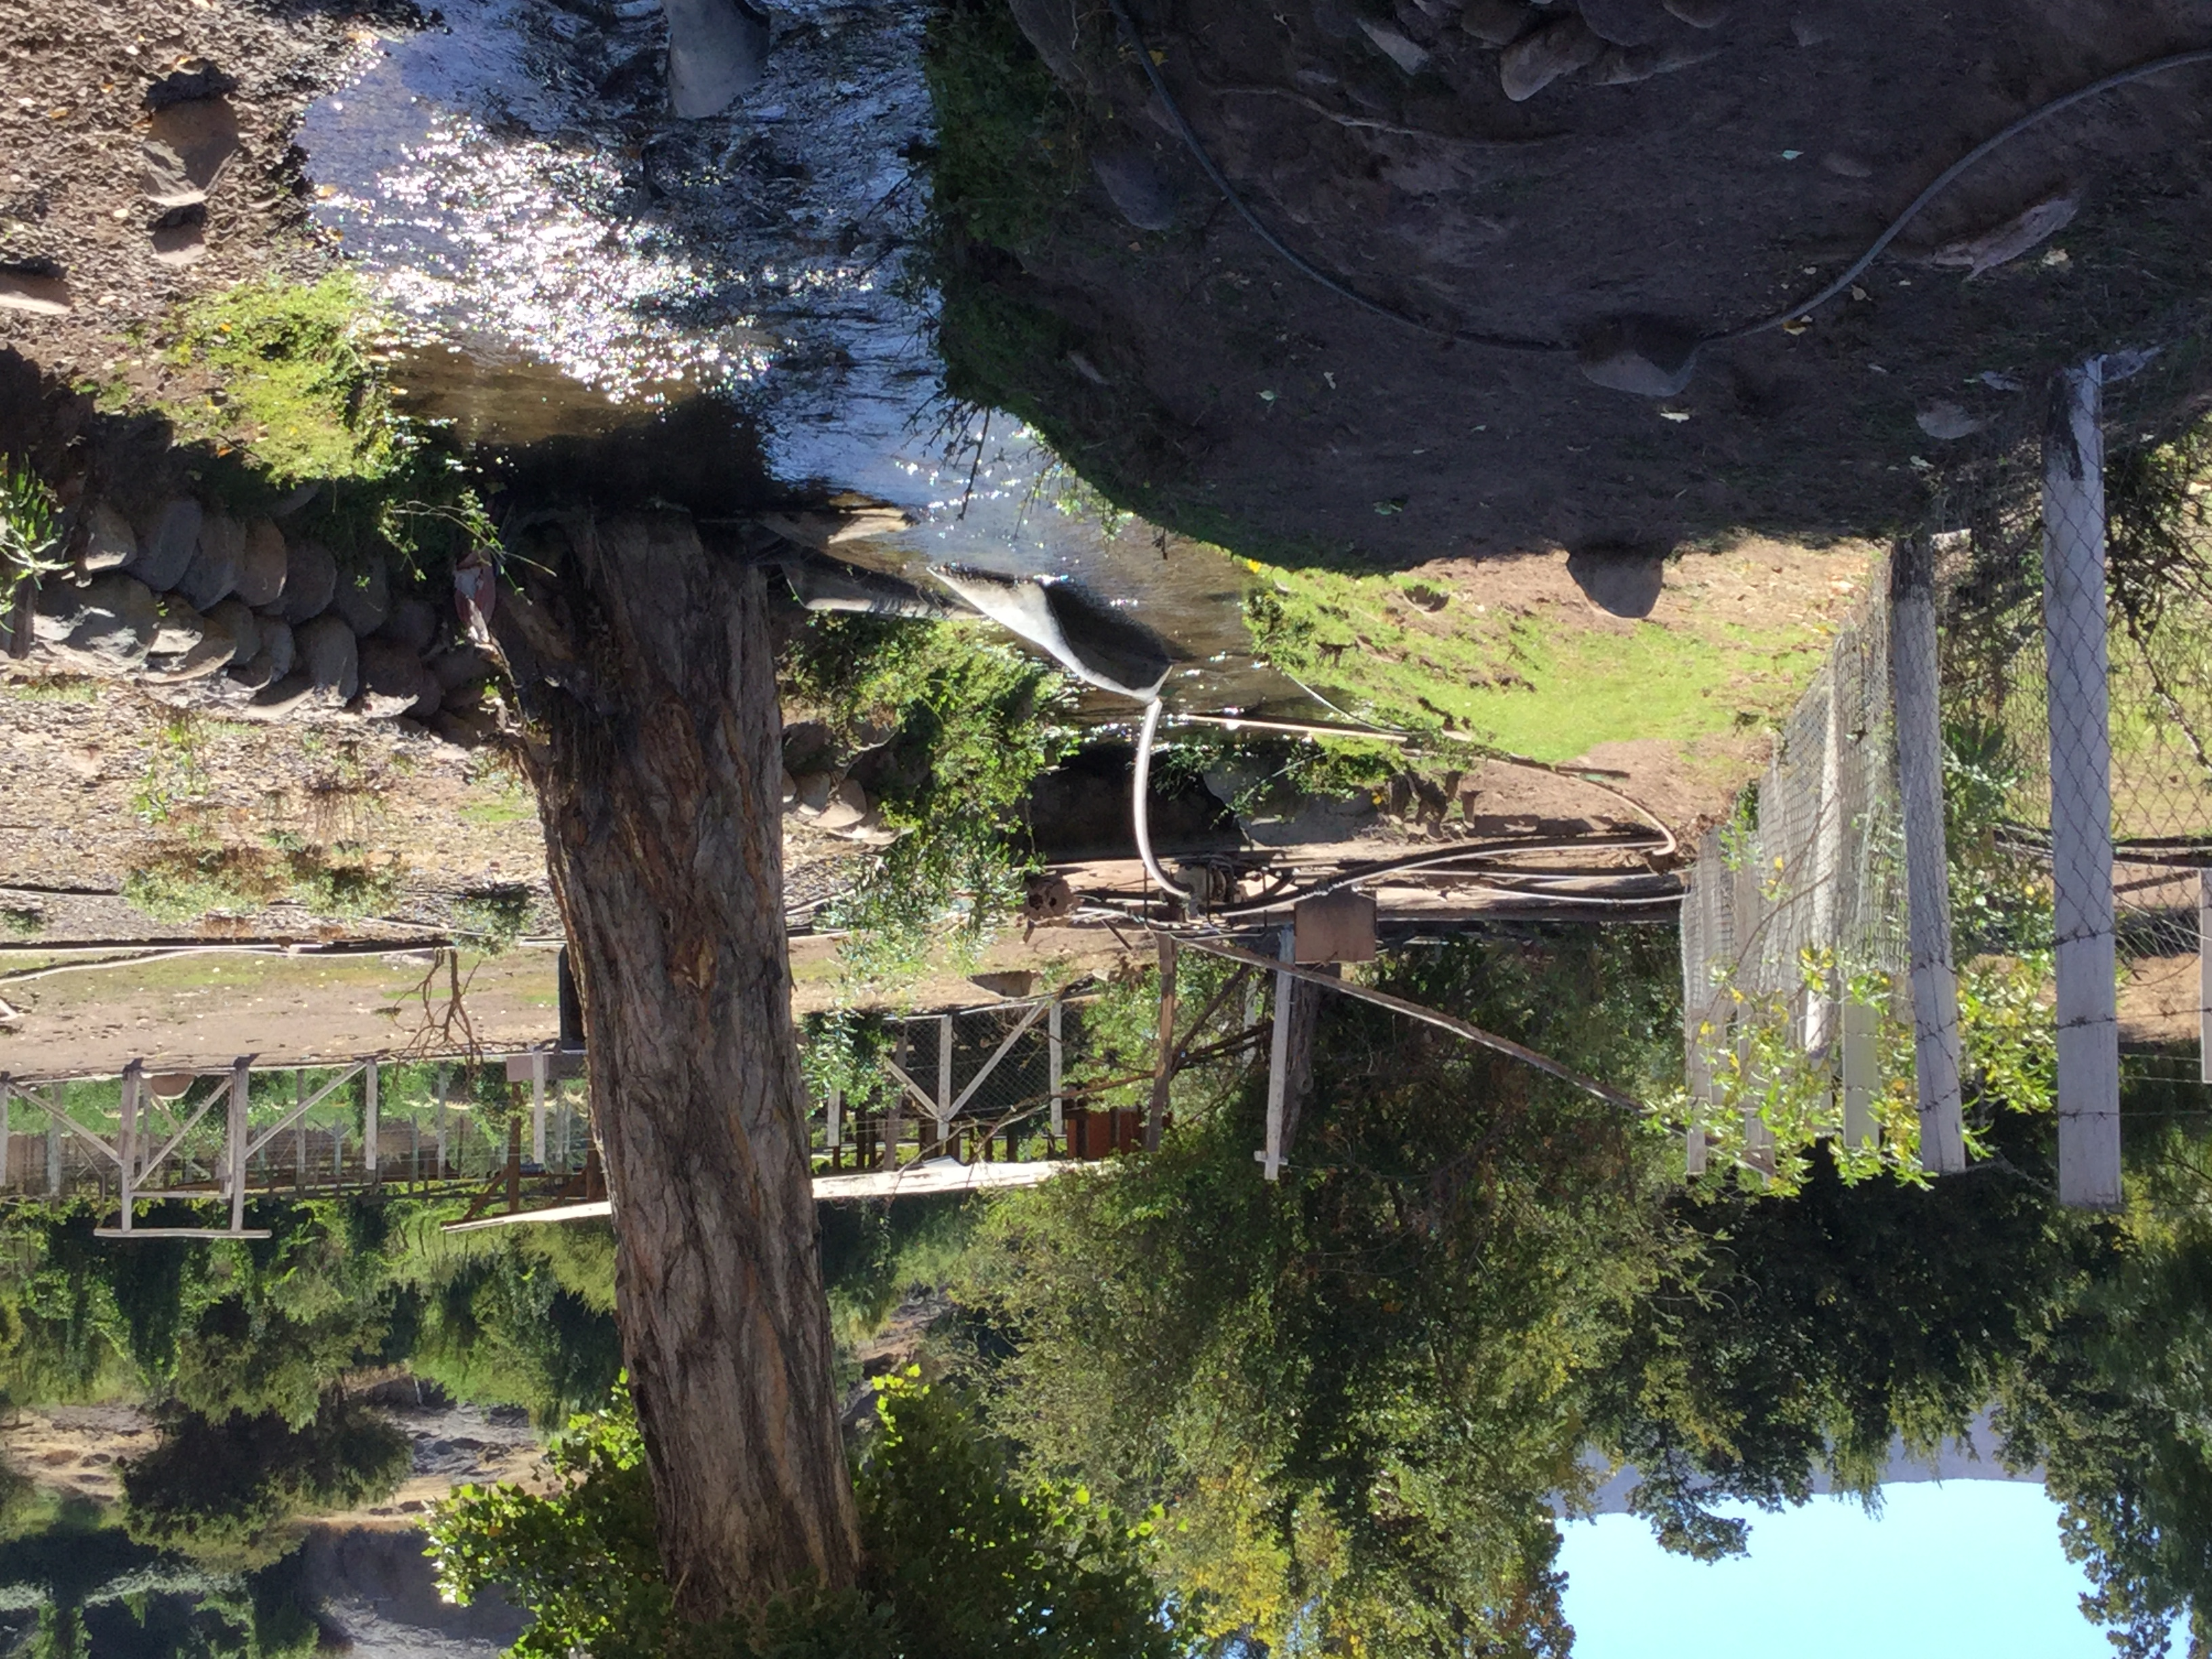
\includegraphics[angle= 180, width=\textwidth]{Foto/a2.jpg} 
\end{subfigure}
\caption{Caracterización de infraestructura hídrica para el S.I.G. de Canal Arboleda Grande, cuenca río Chalinga.}
\end{figure}

\begin{figure}[H]
  \centering
\begin{subfigure}{.45\textwidth}
\hfill
  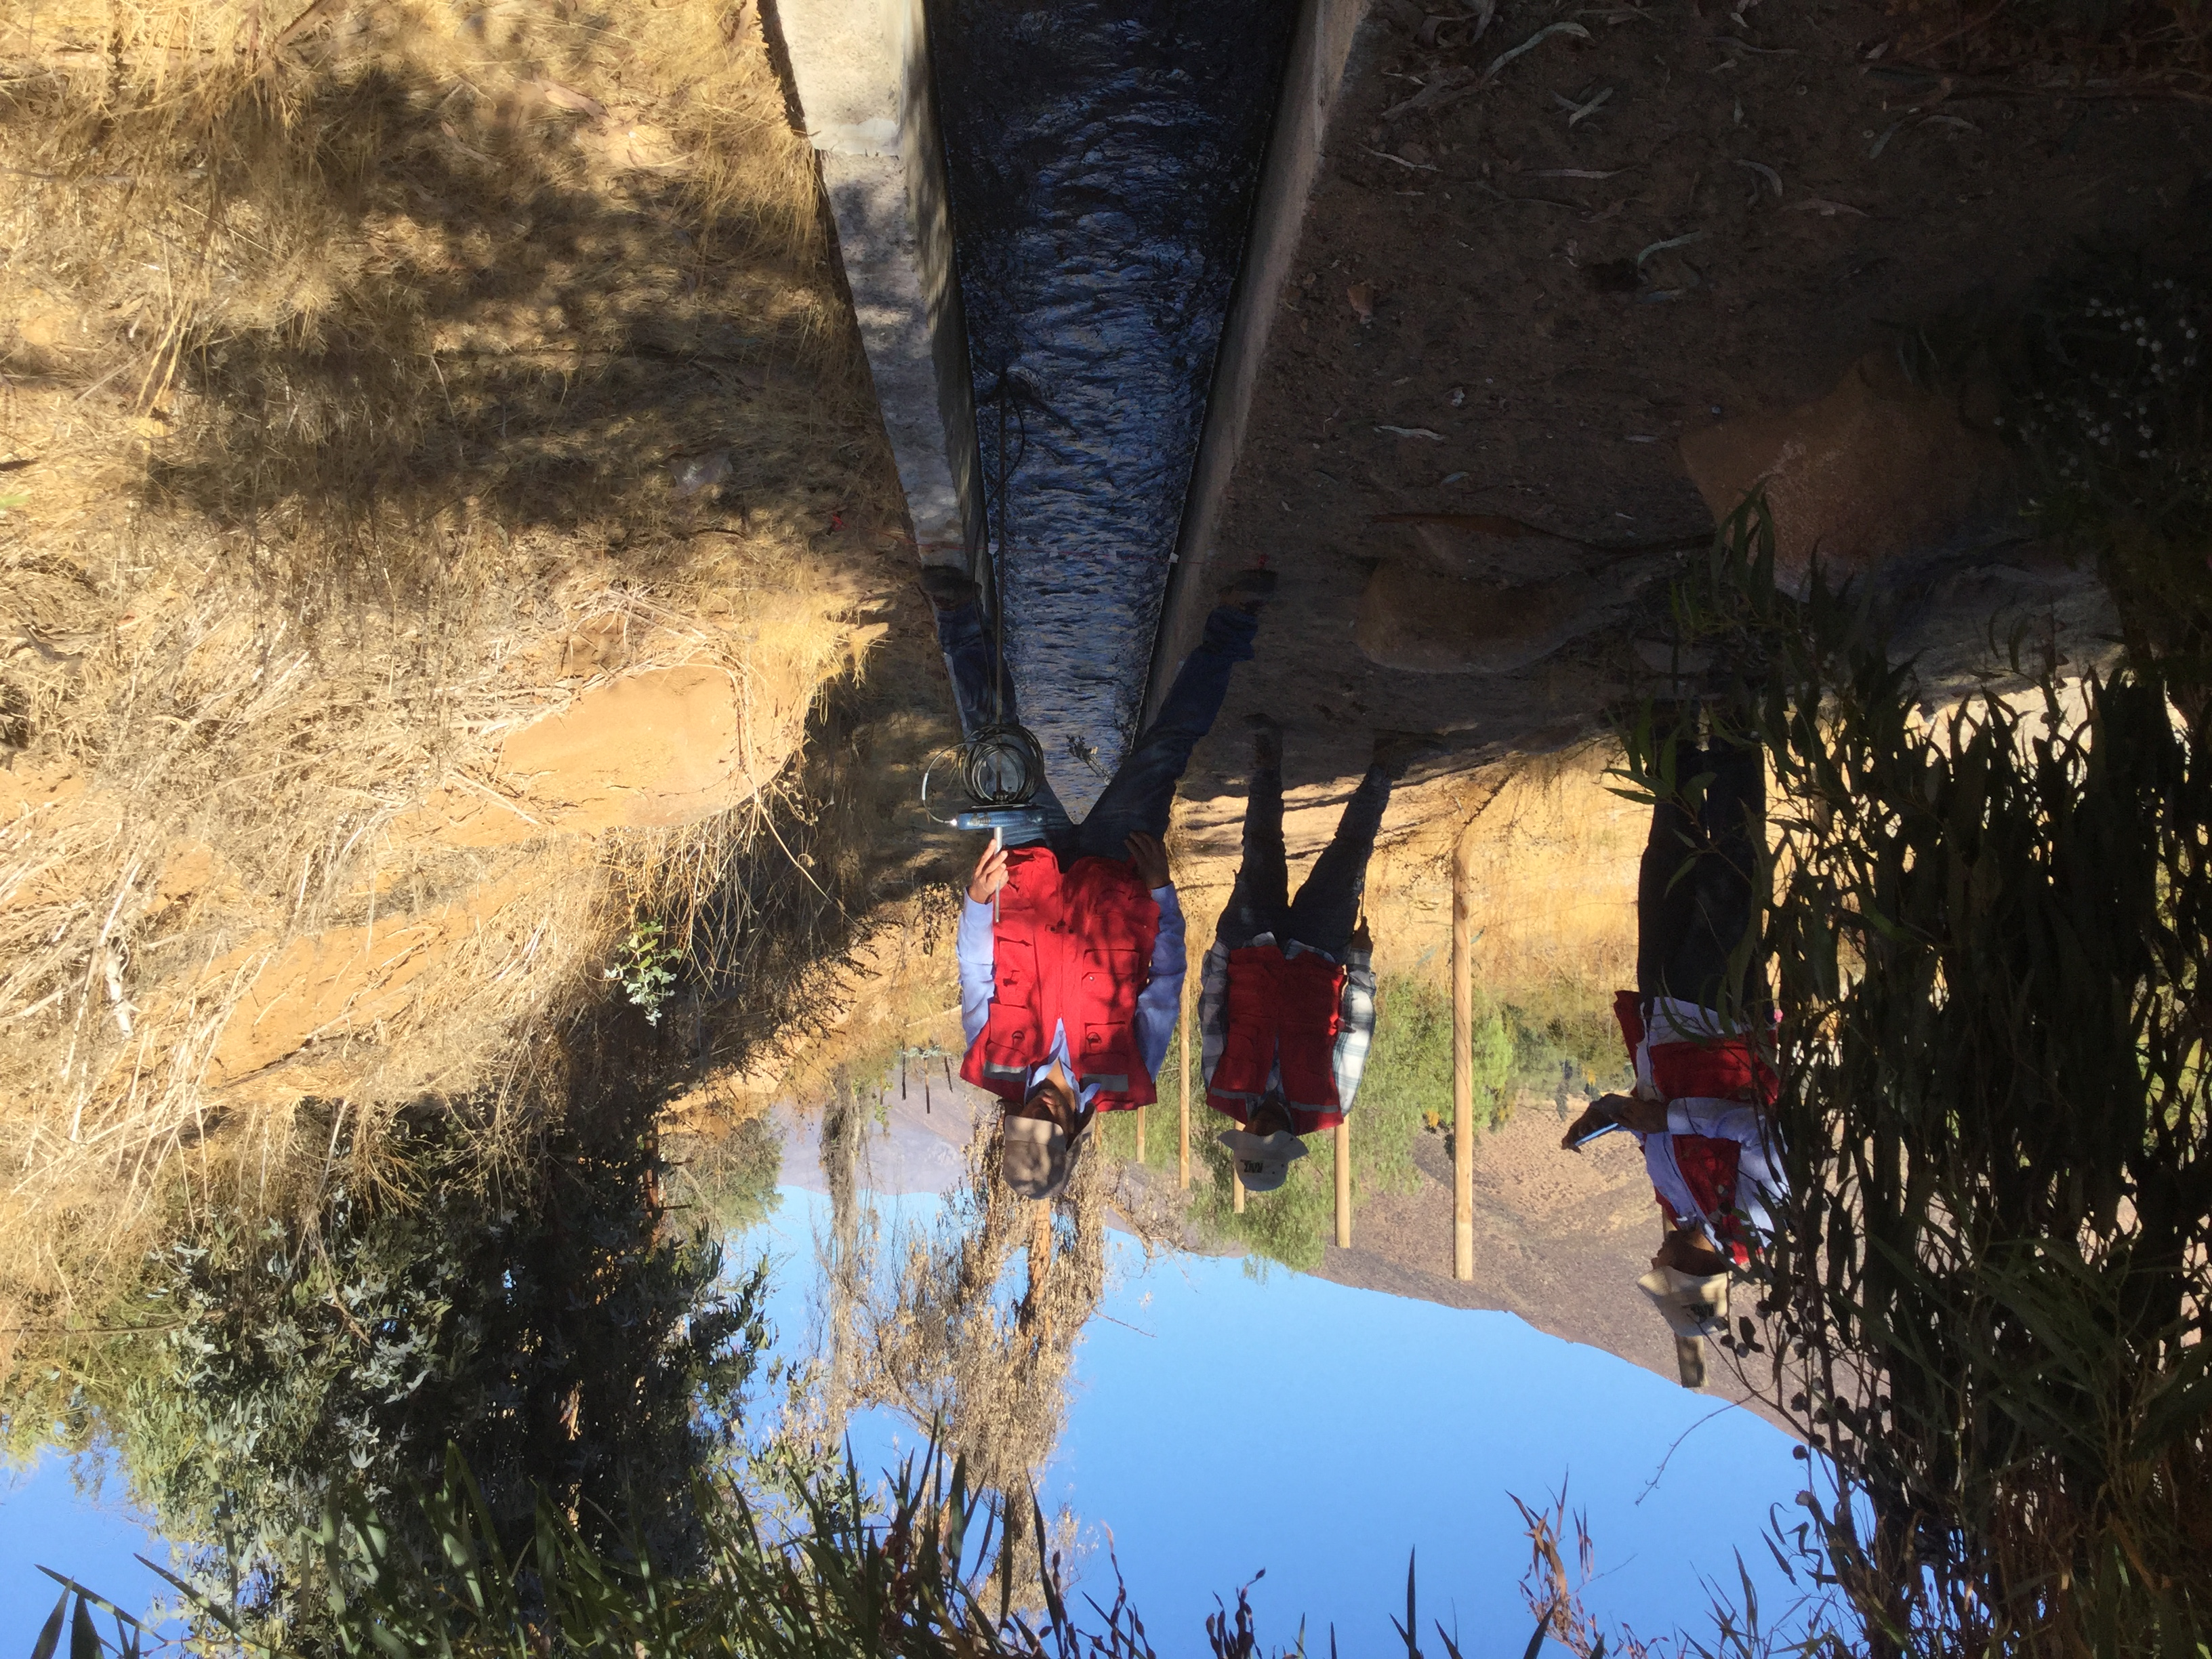
\includegraphics[angle= 180, width=\textwidth]{Foto/a3.jpg}
\end{subfigure}
\hfill
\begin{subfigure}{.45\textwidth}
\hfill
  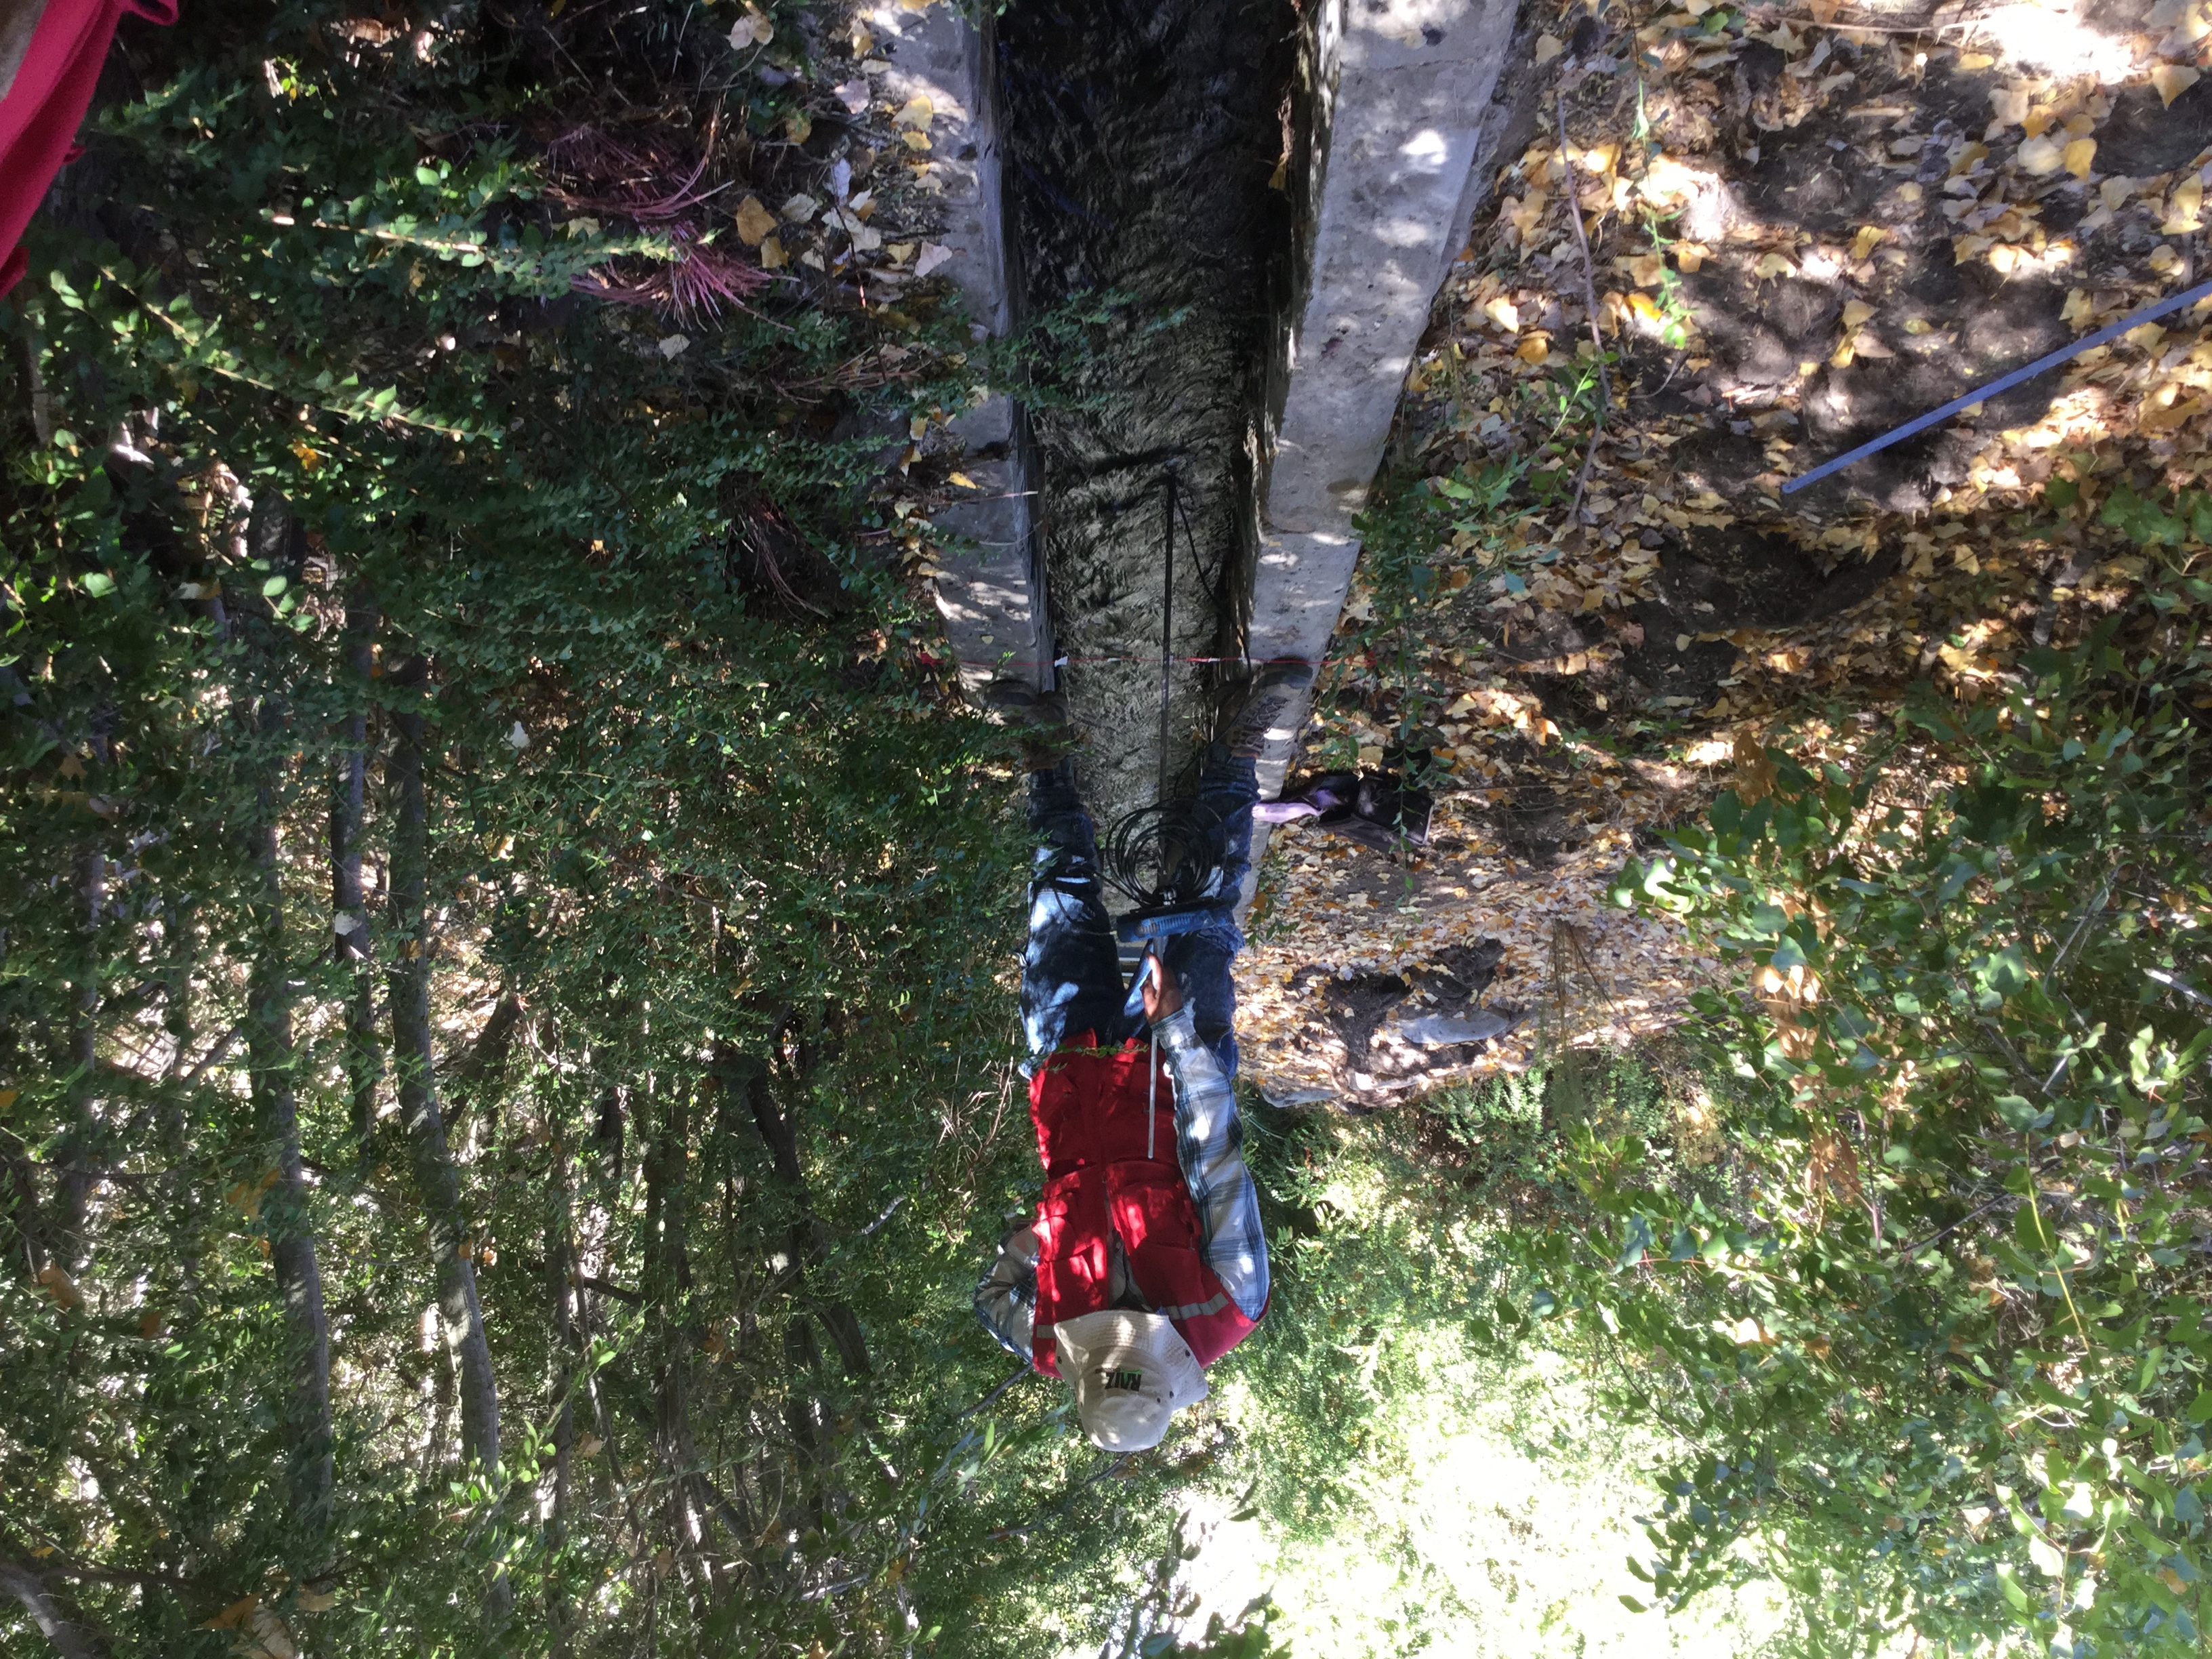
\includegraphics[angle= 180, width=\textwidth]{Foto/a4.jpg} 
\end{subfigure}
\caption{Aforos de caudal Canal Arboleda Grande, cuenca río Chalinga.}
\end{figure}
\clearpage

\textbf{- Comunidad de aguas Huanque.}

\begin{figure}[H]
  \centering
\begin{subfigure}{.45\textwidth}
\hfill
  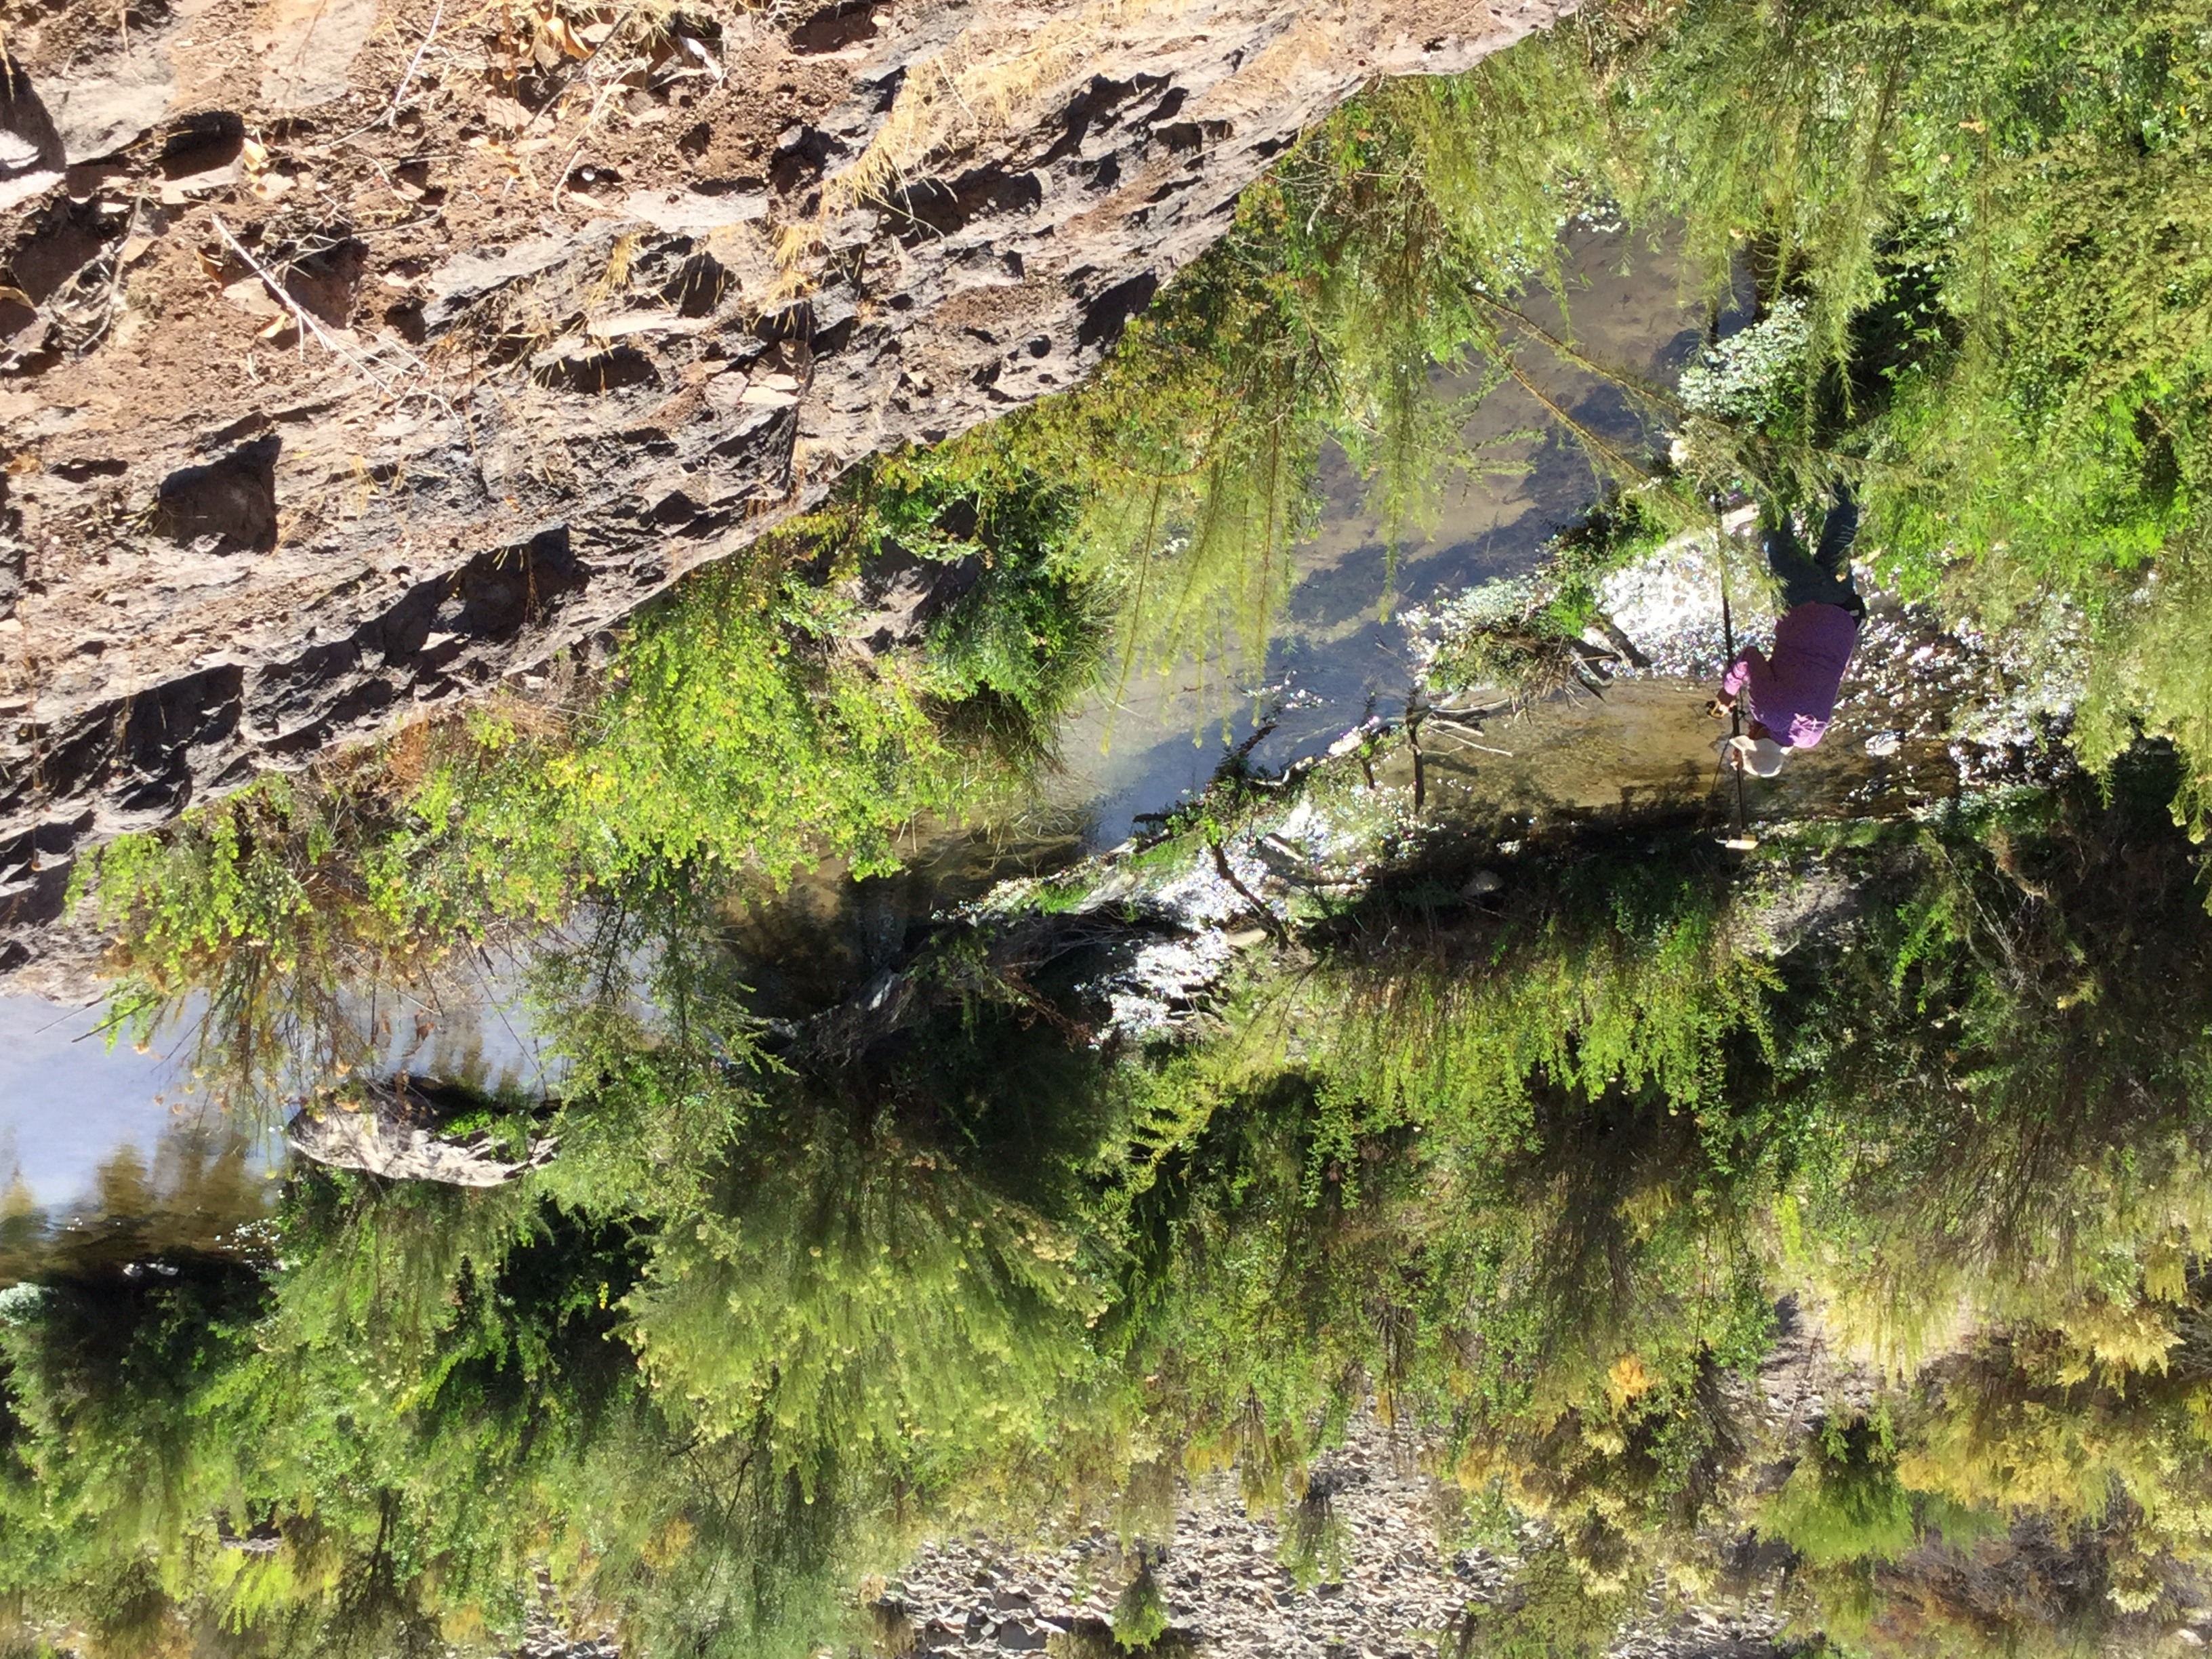
\includegraphics[angle= 180, width=\textwidth]{Foto/h1.jpg}
\end{subfigure}
\hfill
\begin{subfigure}{.45\textwidth}
\hfill
  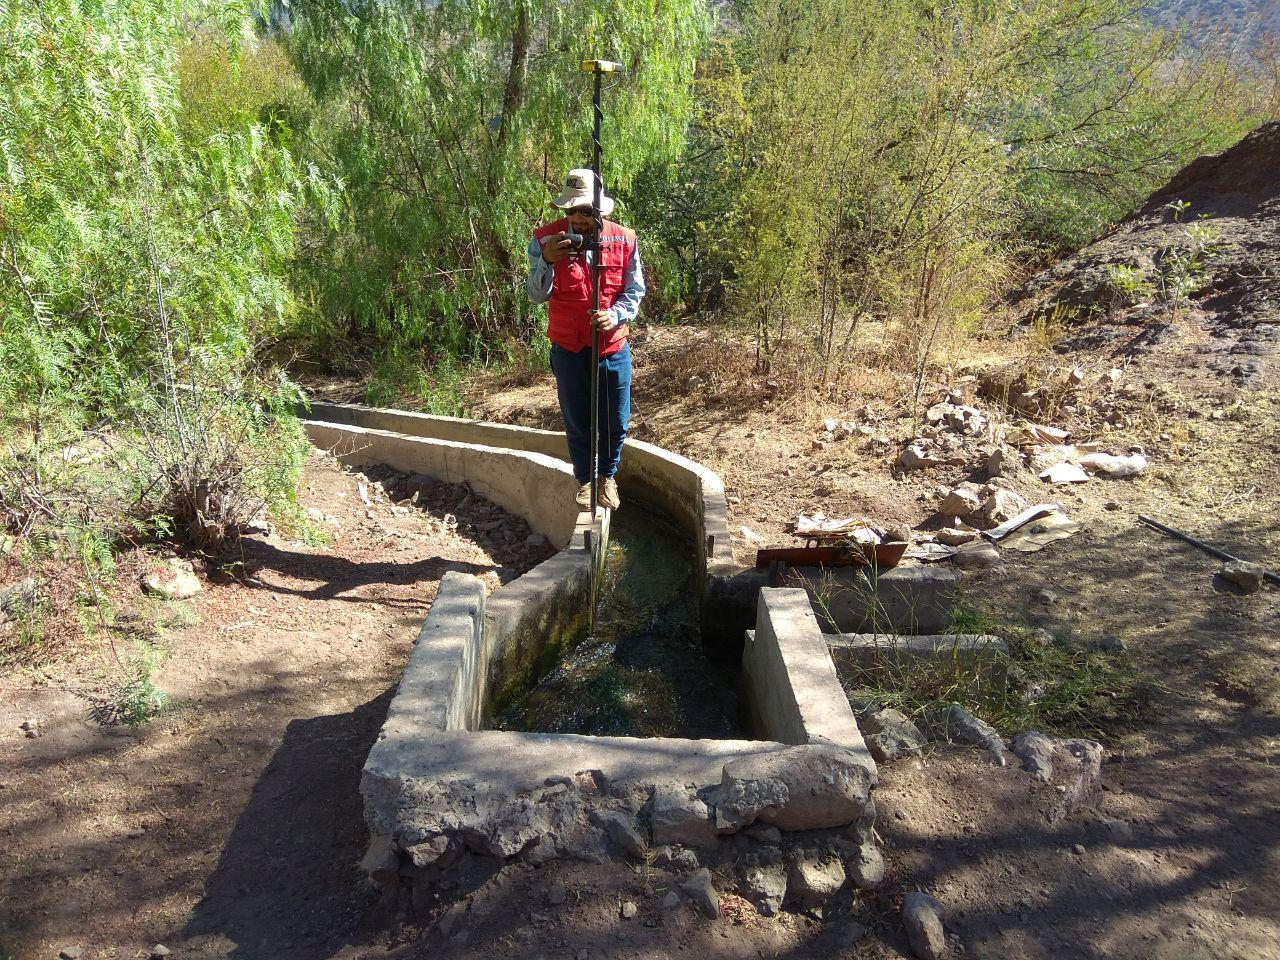
\includegraphics[width=\textwidth]{Foto/h2.jpg} 
\end{subfigure}
\caption{Caracterización de infraestructura hídrica para el S.I.G. de Canal Huanque, cuenca río Chalinga.}
\end{figure}

\begin{figure}[H]
  \centering
\begin{subfigure}{.45\textwidth}
\hfill
  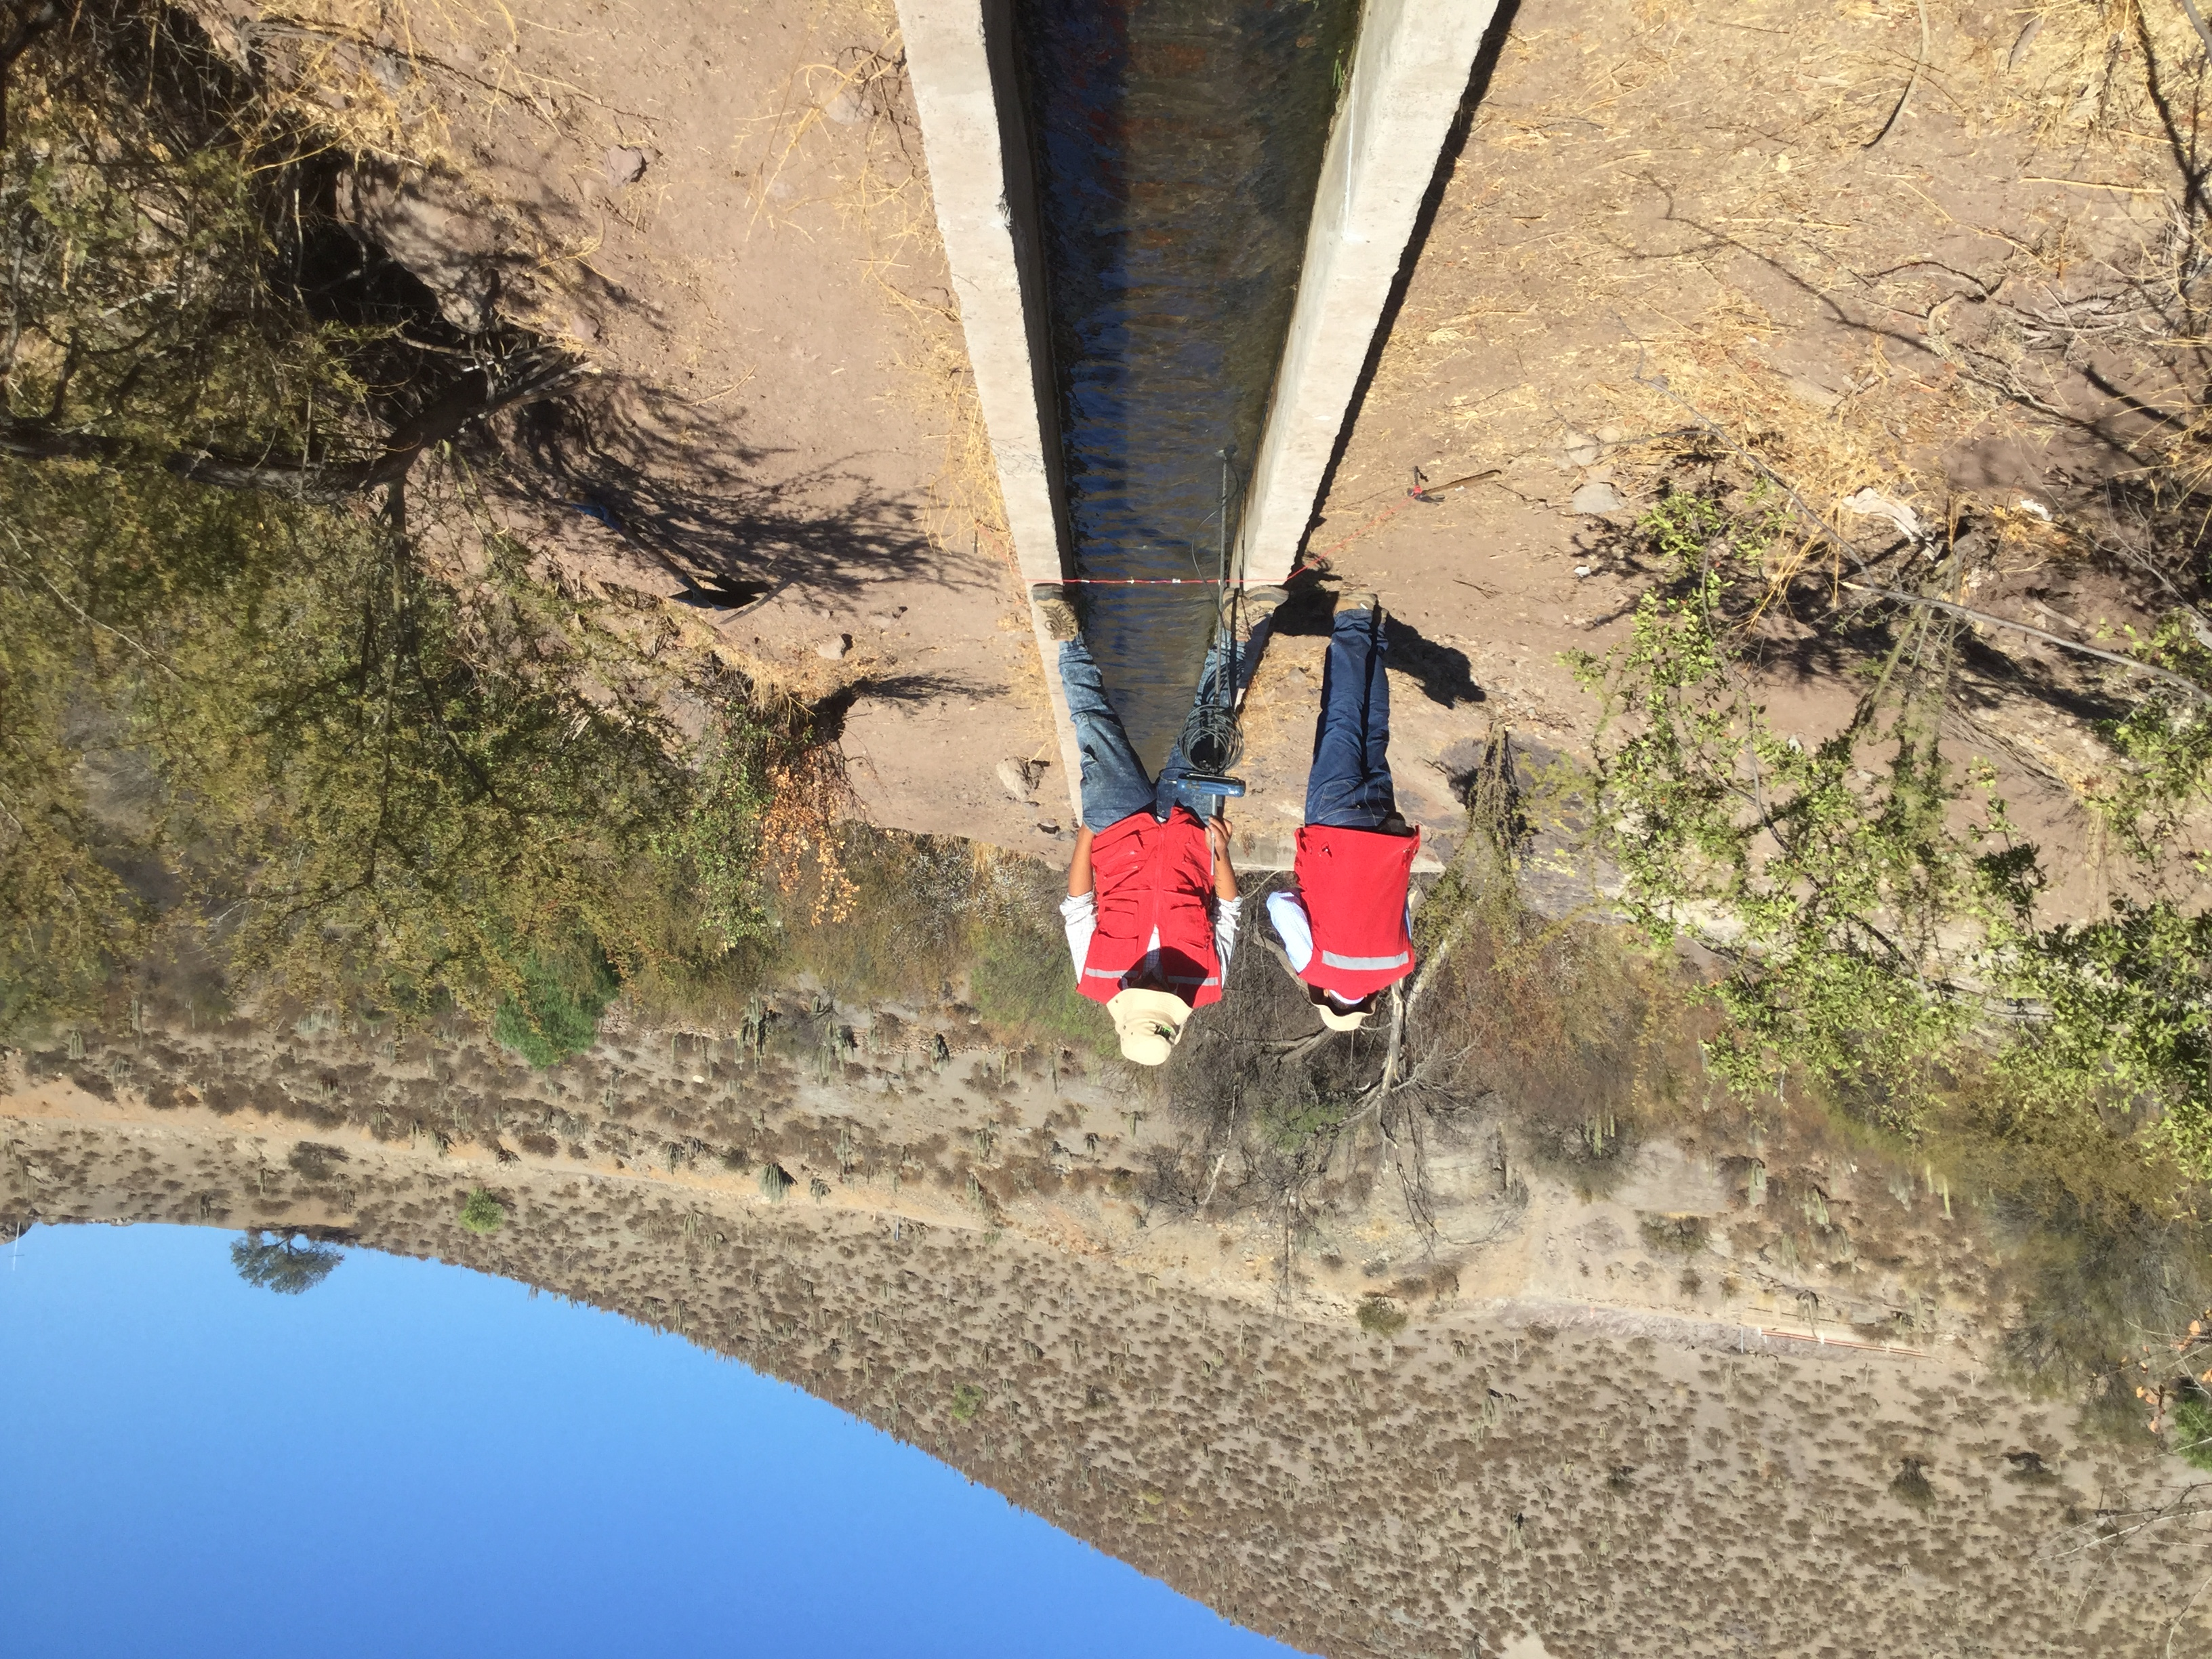
\includegraphics[angle= 180, width=\textwidth]{Foto/h3.jpg}
\end{subfigure}
\hfill
\begin{subfigure}{.45\textwidth}
\hfill
  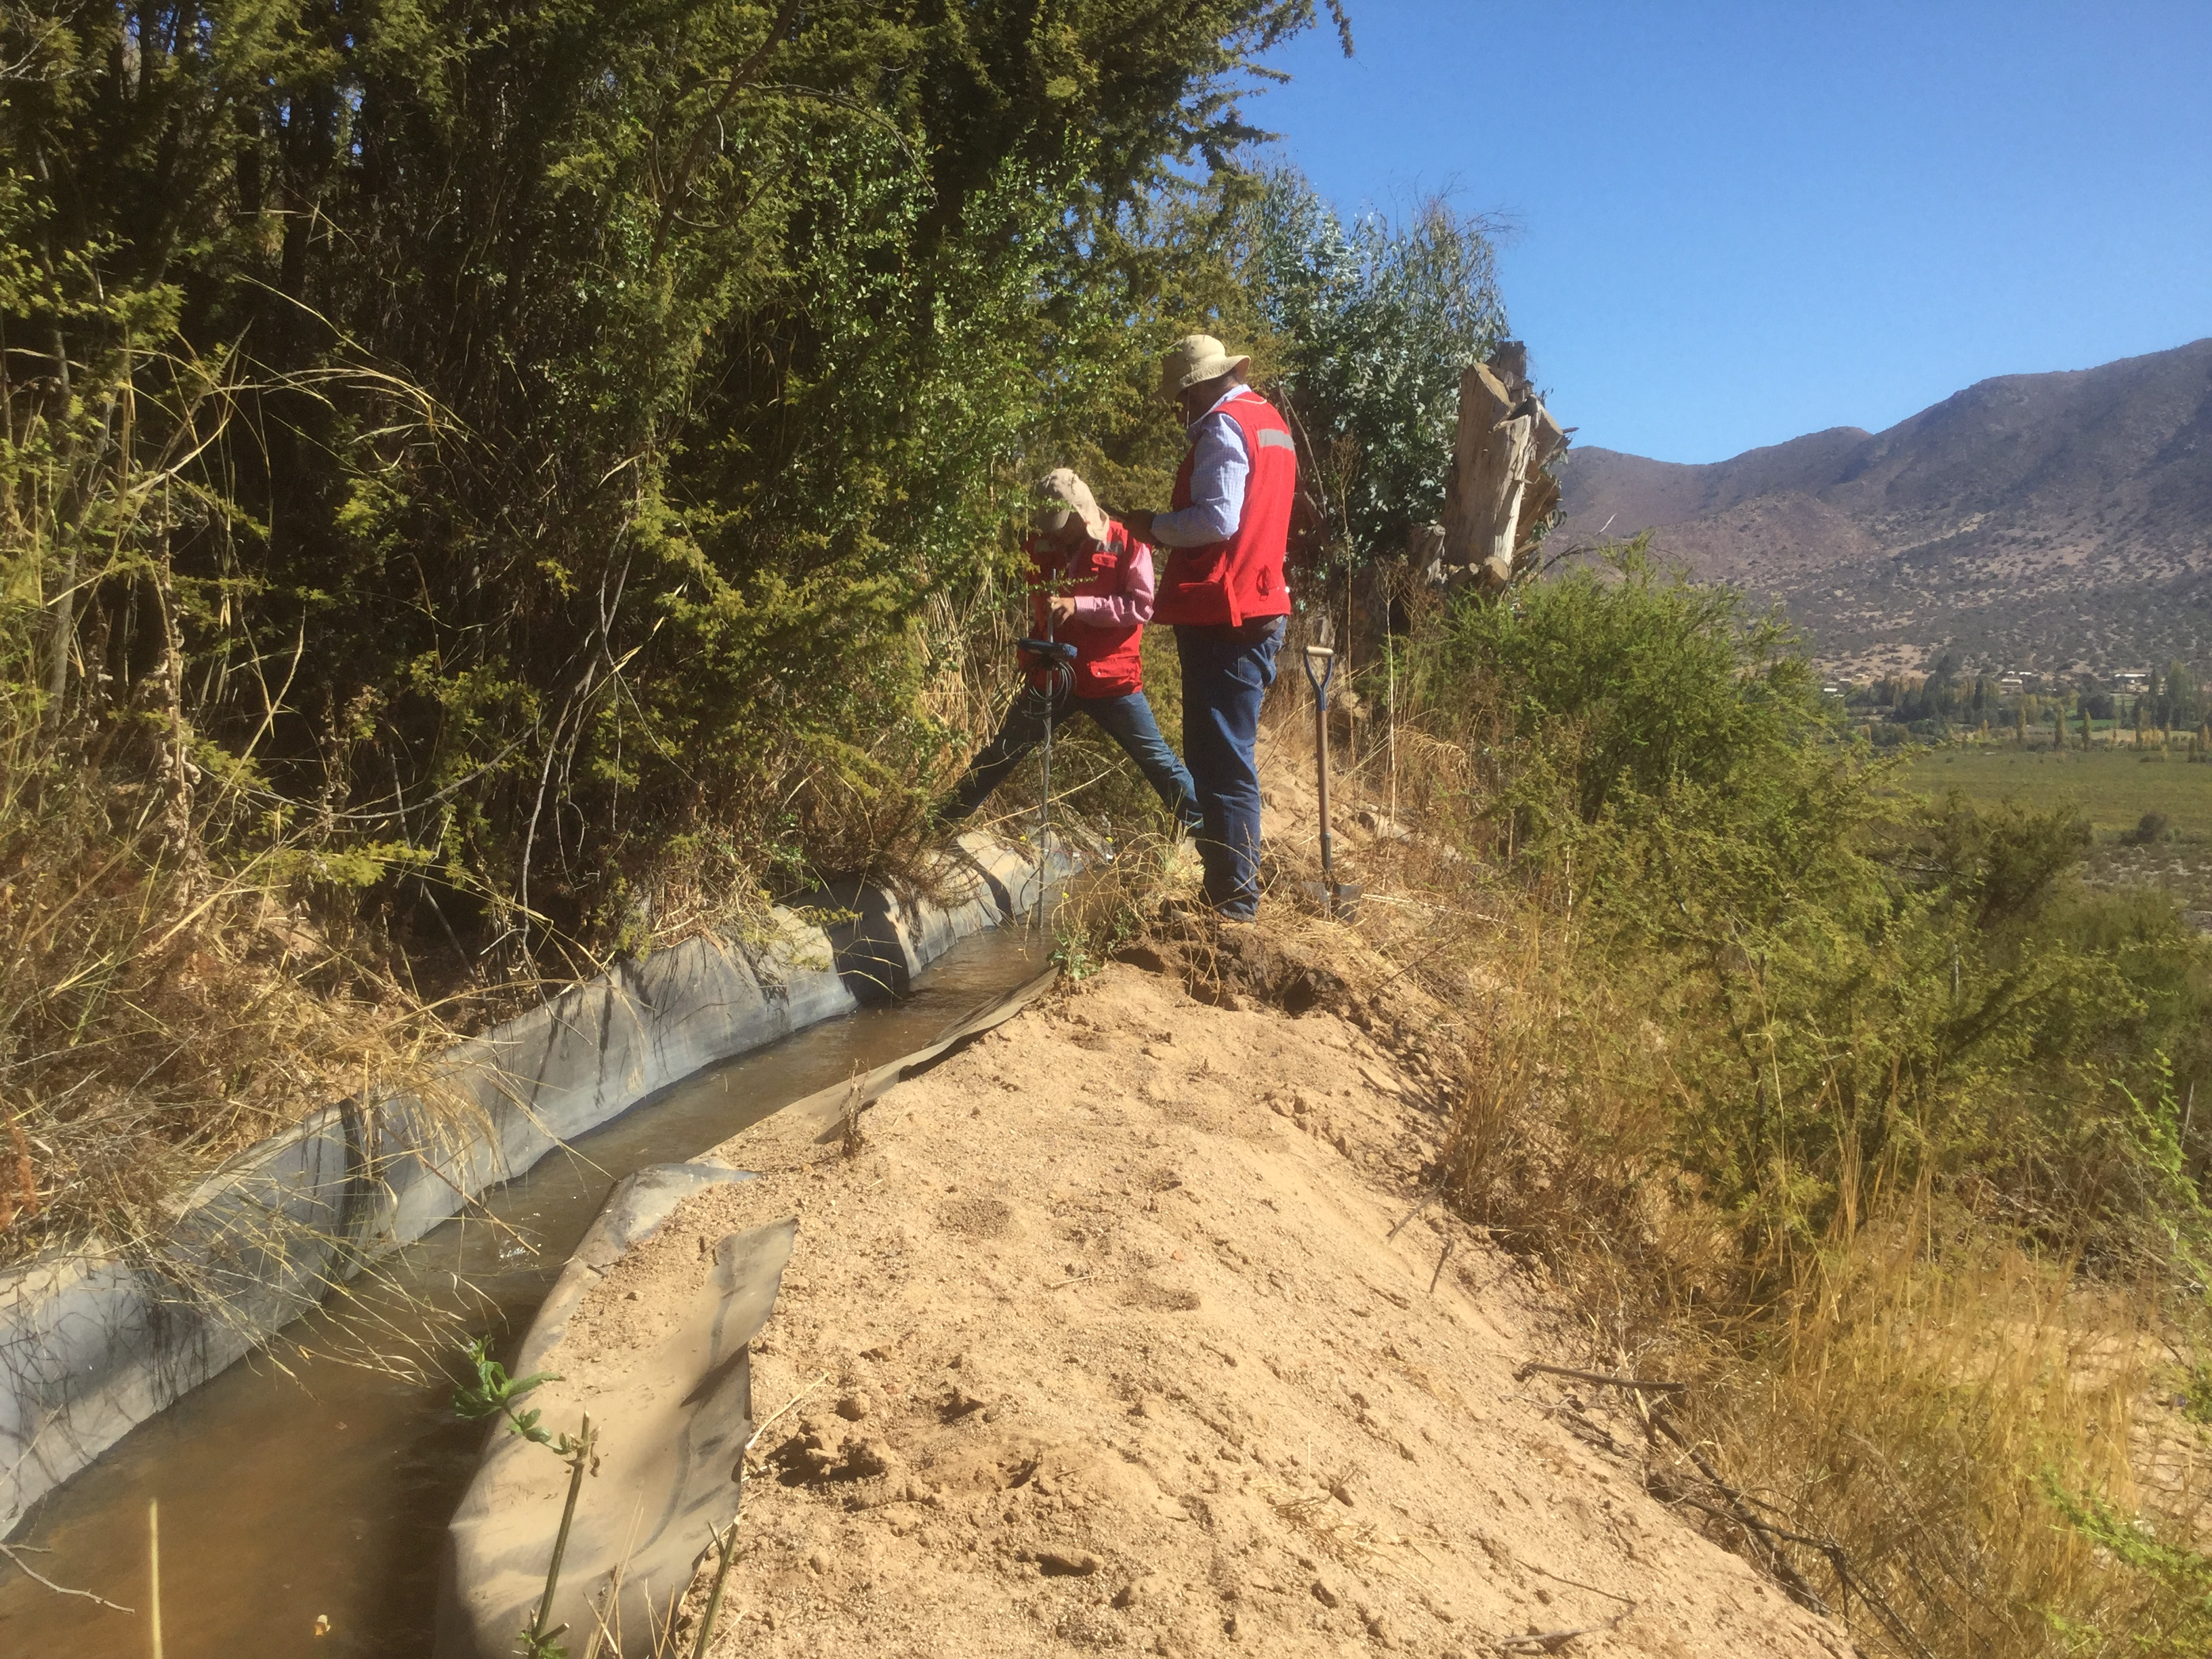
\includegraphics[width=\textwidth]{Foto/h4.jpg} 
\end{subfigure}
\caption{Aforos de caudal Canal Huanque, río Chalinga.}
\end{figure}


\end{document}